\chapter{直升机协同吊挂系统动力学特性及气动干扰分析}
\section{引言}
\section{分层配平法}
\subsection{吊挂物层配平}
\subsection{吊索层优化配平}
\subsection{直升机层差量配平}
\section{配平结果分析}
\section{操纵性分析}
\section{稳定性分析}
\section{气动干扰及其导致的性能变化}
直升机协同吊挂系统是典型的近距离飞行,直升机间、直升机与吊挂物之间、直升机各部件间均存在气动干扰。其中,以前飞时前后排列的直升机间的干扰最为严重。对气动干扰进行分析,可以了解气动干扰产生的机理,有利于减少功率消耗,获得最佳队形,提升系统性能。
\subsection{数值计算条件}
\begin{table}[htb!]
  \caption{直升机1和直升机4的配平结果\label{table:chap_2_1}}
  \begin{tabular}{ccccccccccccc}
    \toprule
    前进比&\multicolumn{2}{c}{0}& \multicolumn{2}{c}{0.04}&\multicolumn{2}{c}{0.06}&\multicolumn{2}{c}{0.08}&\multicolumn{2}{c}{0.1}&\multicolumn{2}{c}{0.14}\\   
    直升机&1&4&1&4&1&4&1&4&1&4&1&4\\
    \midrule
    $\theta_{0,F}$ (\degree)&5.5&5.7&4.0&5.0&3.7&4.8&4.2&4.6&4.1&4.6&4.6&5.2\\
    ${A_{1,F}}$ (\degree)&0.0&0.0&0.4&0.9&0.9&1.2&0.7&1.4&0.9&1.2&1.0&1.0\\
    ${a_{0,F}}$ (\degree)&1.7&1.8&1.4&1.7&1.5&1.7&1.8&1.6&1.8&1.6&1.8&1.5\\
    ${a_{1,F}}$ (\degree)&0.0&0.0&0.6&1.0&1.2&1.5&1.2&1.7&1.5&1.7&1.9&1.9\\
    $\theta_{0,R}$ (\degree)& 5.6 & 5.8 & 4.5 & 5.3 & 4.4 & 5.7 & 4.7 & 5.8 & 4.9 & 5.7 & 5.4 & 6.1\\
    ${A_{1,R}}$ (\degree)& 0.0 & 0.0 & 0.4 & 0.7 & 0.8 & 1.1 & 0.7 & 1.2 & 0.7 & 1.1 & 0.7 & 0.9 \\
    ${a_{0,R}}$ (\degree)& 1.7 & 1.8 & 1.7 & 1.8 & 1.8 & 2.1 & 2.0 & 2.1 & 2.2 & 2.1 & 2.2 & 2.0 \\
    ${a_{1,R}}$ (\degree)& 0.0 & 0.0 & 0.7 & 1.0 & 1.2 & 1.5 & 1.3 & 1.8 & 1.6 & 1.8 & 2.1 & 2.1 \\
    $\theta$ (\degree)& 3.4 & -3.9 & 2.8 & -5.3 & 1.8 & -7.2 & 0.5 & -7.7 & -0.8 & -8.9 & -4.3 & -11.4 \\
    \bottomrule
  \end{tabular}
\end{table}
协同吊挂系统的气动干扰研究是在稳定飞行状态下开展的。稳定飞行状态下的状态量基于前文提出的混合优化配平算法配平得到。
本文研究的四纵列式直升机协同吊挂系统是“2-lead”队形的,假设吊挂负载均匀分配给各直升机,那么稳定飞行状态下后侧直升机(直升机1、2)的纵向配平量相等,前侧直升机(直升机3、4)的纵向配平量相等。下表以直升机1、直升机3为例给出了配平结果。其中,${\theta _{0,F}}$、${\theta _{0,R}}$分别为前、后旋翼的总距,$\theta $是俯仰角,${A_{1,F}}$、${A_{1,R}}$是横向周期变距,${a_{0,F}}$、${a_{0,R}}$是前、后旋翼挥舞角写成傅里叶级数时的常数项,${a_{1,F}}$、${a_{1,R}}$是前、后旋翼挥舞角写成傅里叶级数时的cos项。值得一提的是,纵列式直升机纵向运动是通过前后旋翼的总距差动实现的,所以纵向周期变距等于0。此外,直升机1和直升机4的滚转角为-4 \degree,直升机2和直升机3的滚转角为4 \degree。直升机1、2、3、4和吊挂物在地轴系下的位置依次为[-1.8, -1.8, -3.7],[-1.8, 1.8, -3.7],[1.8, 1.8, -3.7],[1.8, -1.8, -3.7] 和 [0, 0, 0]。

值得一提的是,以稳定飞行状态为基础计算气动干扰是必要的。若没有配平,而是随意选择各直升机姿态角和旋翼操纵量开展气动干扰分析,此时的计算结果是没有意义的,不能体现直升机协同吊挂系统的真实飞行状态。表\ref{table:chap_2_1}所示的配平量为涡方法提供了系统初始状态量,保证了气动干扰分析和性能计算的可靠度。

\begin{figure}[!htb]
  \centering
  \subfloat[X-Z平面]{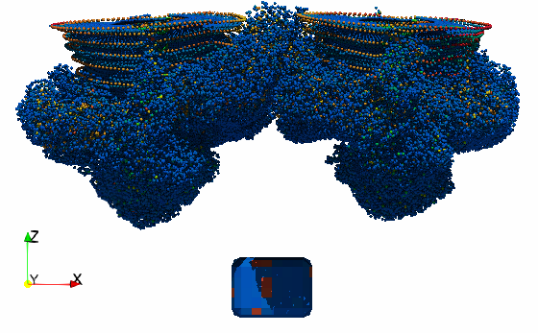
\includegraphics[width=6cm]{fig/figure_chap3/chap_3_5_1_1_1.png}}\quad 
  \subfloat[X-Y平面]{\includegraphics[width=5cm]{fig/figure_chap3/chap_3_5_1_1_2.png}}\\
  \caption{悬停时直升机协同吊挂系统尾迹结构}
  \label{fig:chap3_5_1_1_1}
\end{figure}

\begin{figure}[!htb]
  \centering
  \subfloat[X-Z平面]{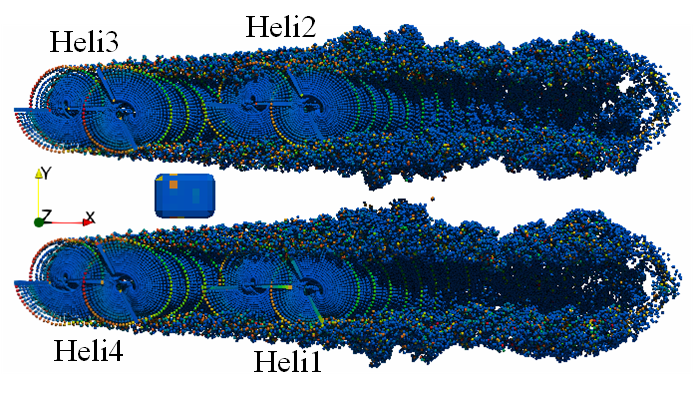
\includegraphics[width=6cm]{fig/figure_chap3/chap_3_5_1_2_1.png}}\quad 
  \subfloat[X-Y平面]{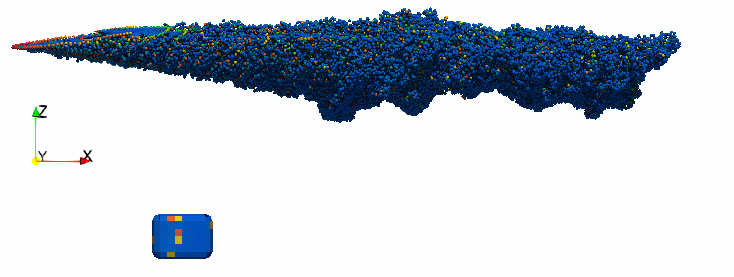
\includegraphics[width=8cm]{fig/figure_chap3/chap_3_5_1_2_2.png}}\\
  \caption{前进比0.1时直升机协同吊挂系统尾迹结构}
  \label{fig:chap3_5_1_1_2}
\end{figure}

\subsection{不同飞行速度下的气动干扰}
基于表\ref{table:chap_2_1}中的配平结果,开展了稳定飞行状态下的气动干扰特性分析。图\ref{fig:chap3_5_1_1_1}和图\ref{fig:chap3_5_1_1_2}分别给出了悬停、前进比0.1(前飞速度10 m/s)时的尾迹结构。可以看出,悬停时四个纵列式直升机间几乎没有干扰。前进比0.1时存在气动干扰,其中以前后排列的直升机间的干扰最大。此外,可以发现无论是悬停还是前进比0.1时,吊挂物都没有浸入旋翼尾迹中。这说明本文研究的四纵列式直升机协同吊挂系统,直升机对吊挂物的气动干扰不大。并且,从表\ref{table:chap_2_1}的配平结果、图\ref{fig:chap3_5_1_1_1}和图\ref{fig:chap3_5_1_1_2}的尾迹结构可以看出,直升机1和2的配平结果及气动干扰情况是相似的,直升机3和4的配平结果及气动干扰情况也是相似的。因此,下文以直升机1和直升机4为例开展讨论和分析。

\begin{figure}[!htb]
  \centering
  \subfloat[悬停时XY截面的速度场]{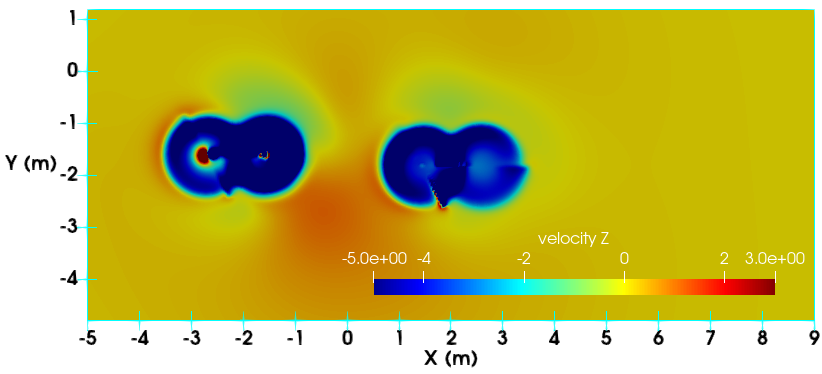
\includegraphics[width=5.5cm]{fig/figure_chap3/chap_3_5_1_3.png}}\quad 
  \subfloat[悬停时XZ截面的速度场]{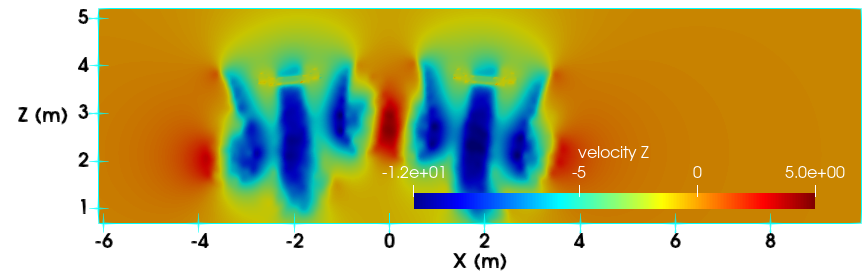
\includegraphics[width=8.5cm]{fig/figure_chap3/chap_3_5_1_4.png}}\\
  \subfloat[前飞速度6 m/s时XY截面的速度场]{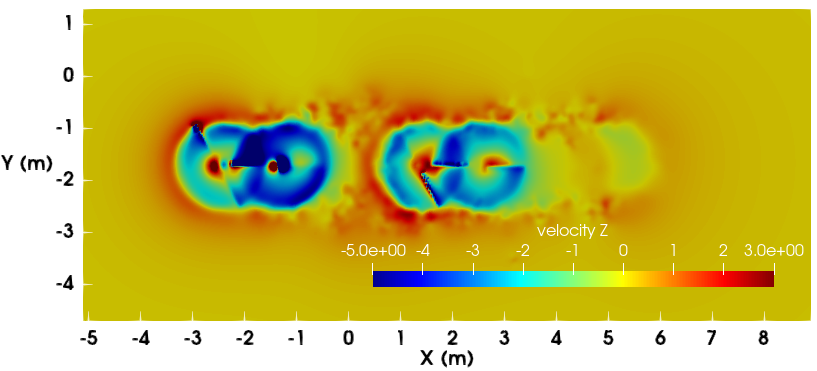
\includegraphics[width=5.5cm]{fig/figure_chap3/chap_3_5_1_5.png}}\quad 
  \subfloat[前飞速度6 m/s时XZ截面的速度场]{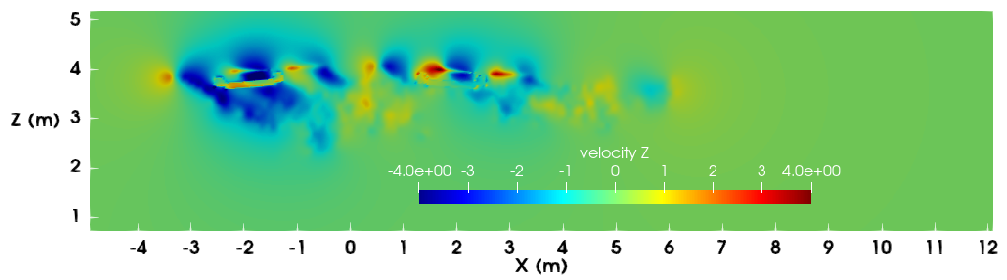
\includegraphics[width=8.5cm]{fig/figure_chap3/chap_3_5_1_6.png}}\\
  \subfloat[前飞速度12 m/s时XY截面的速度场]{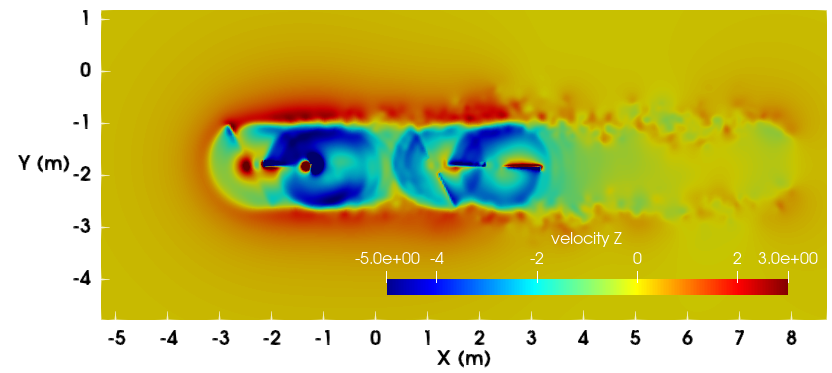
\includegraphics[width=5.5cm]{fig/figure_chap3/chap_3_5_1_7.png}}\quad 
  \subfloat[前飞速度12 m/s时XZ截面的速度场]{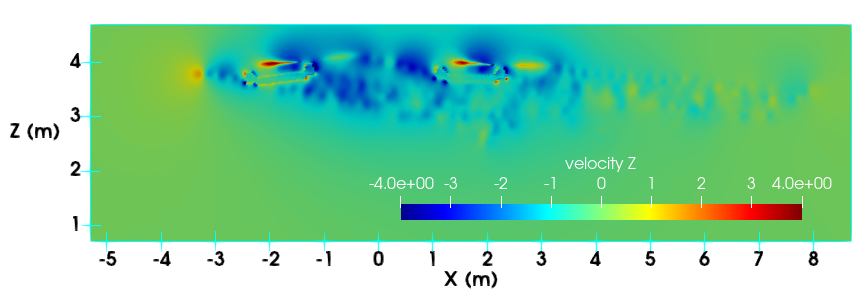
\includegraphics[width=8.5cm]{fig/figure_chap3/chap_3_5_1_8.png}}\\
  \caption{直升机协同吊挂系统不同飞行状态下的速度场}
  \label{fig:chap3_5_1_2}
\end{figure}
 
图\ref{fig:chap3_5_1_2}给出了直升机1和直升机4不同飞行状态下的速度场。悬停时,如图\ref{fig:chap3_5_1_2}(a)(b)所示,旋翼下洗速度主要存在于桨盘到桨盘2倍旋翼直径以下的区域。上洗速度是涡扩散和上卷引起的。其中,由于前后直升机尾迹的重合,坐标(0,0,3m)处的上洗速度是(±3.8m,0,2m)处的2倍。尾迹倾斜与直升机自身的姿态角有关。悬停时直升机1和直升机4的姿态角分别为3.4 \degree 和-3.9 \degree,所以直升机4的尾迹向左倾斜,直升机1的尾迹向右倾斜。

前进比0.06时,如图\ref{fig:chap3_5_1_2}(c)(d)所示,尾迹朝来流方向倾斜,由于上卷桨尖涡的作用,给纵列式直升机1的前旋翼带来了一定的上洗速度。这尽管有利于增加直升机1千旋翼的迎角,但上卷的桨尖涡作用会给旋翼带来更复杂的工作环境。前进比0.1时,随着飞行速度的增加,直升机4的旋翼下洗流对直升机1的干扰越来越大。相比无干扰时,这势必会导致直升机1旋翼拉力的减小和功率消耗的增加。

可见,对于本文研究的四纵列式直升机协同吊挂系统,悬停时直升机之间、直升机与吊挂物之间几乎不存在气动干扰。随着飞行速度的增加,气动干扰变得越来越严重,以前后排列的直升机间的干扰更甚。此外,可以发现协同吊挂系统间的气动干扰比较复杂,且不同前飞速度下对性能的影响往往是不同的。为了减少协同吊挂系统中的气动干扰、提高性能,下文重点分析气动干扰的变化及其影响因子。其中,为分析方便,固定前进比为0.1,对应协同吊挂系统中气动干扰较为严重的情况。

\begin{figure}
  \centering
  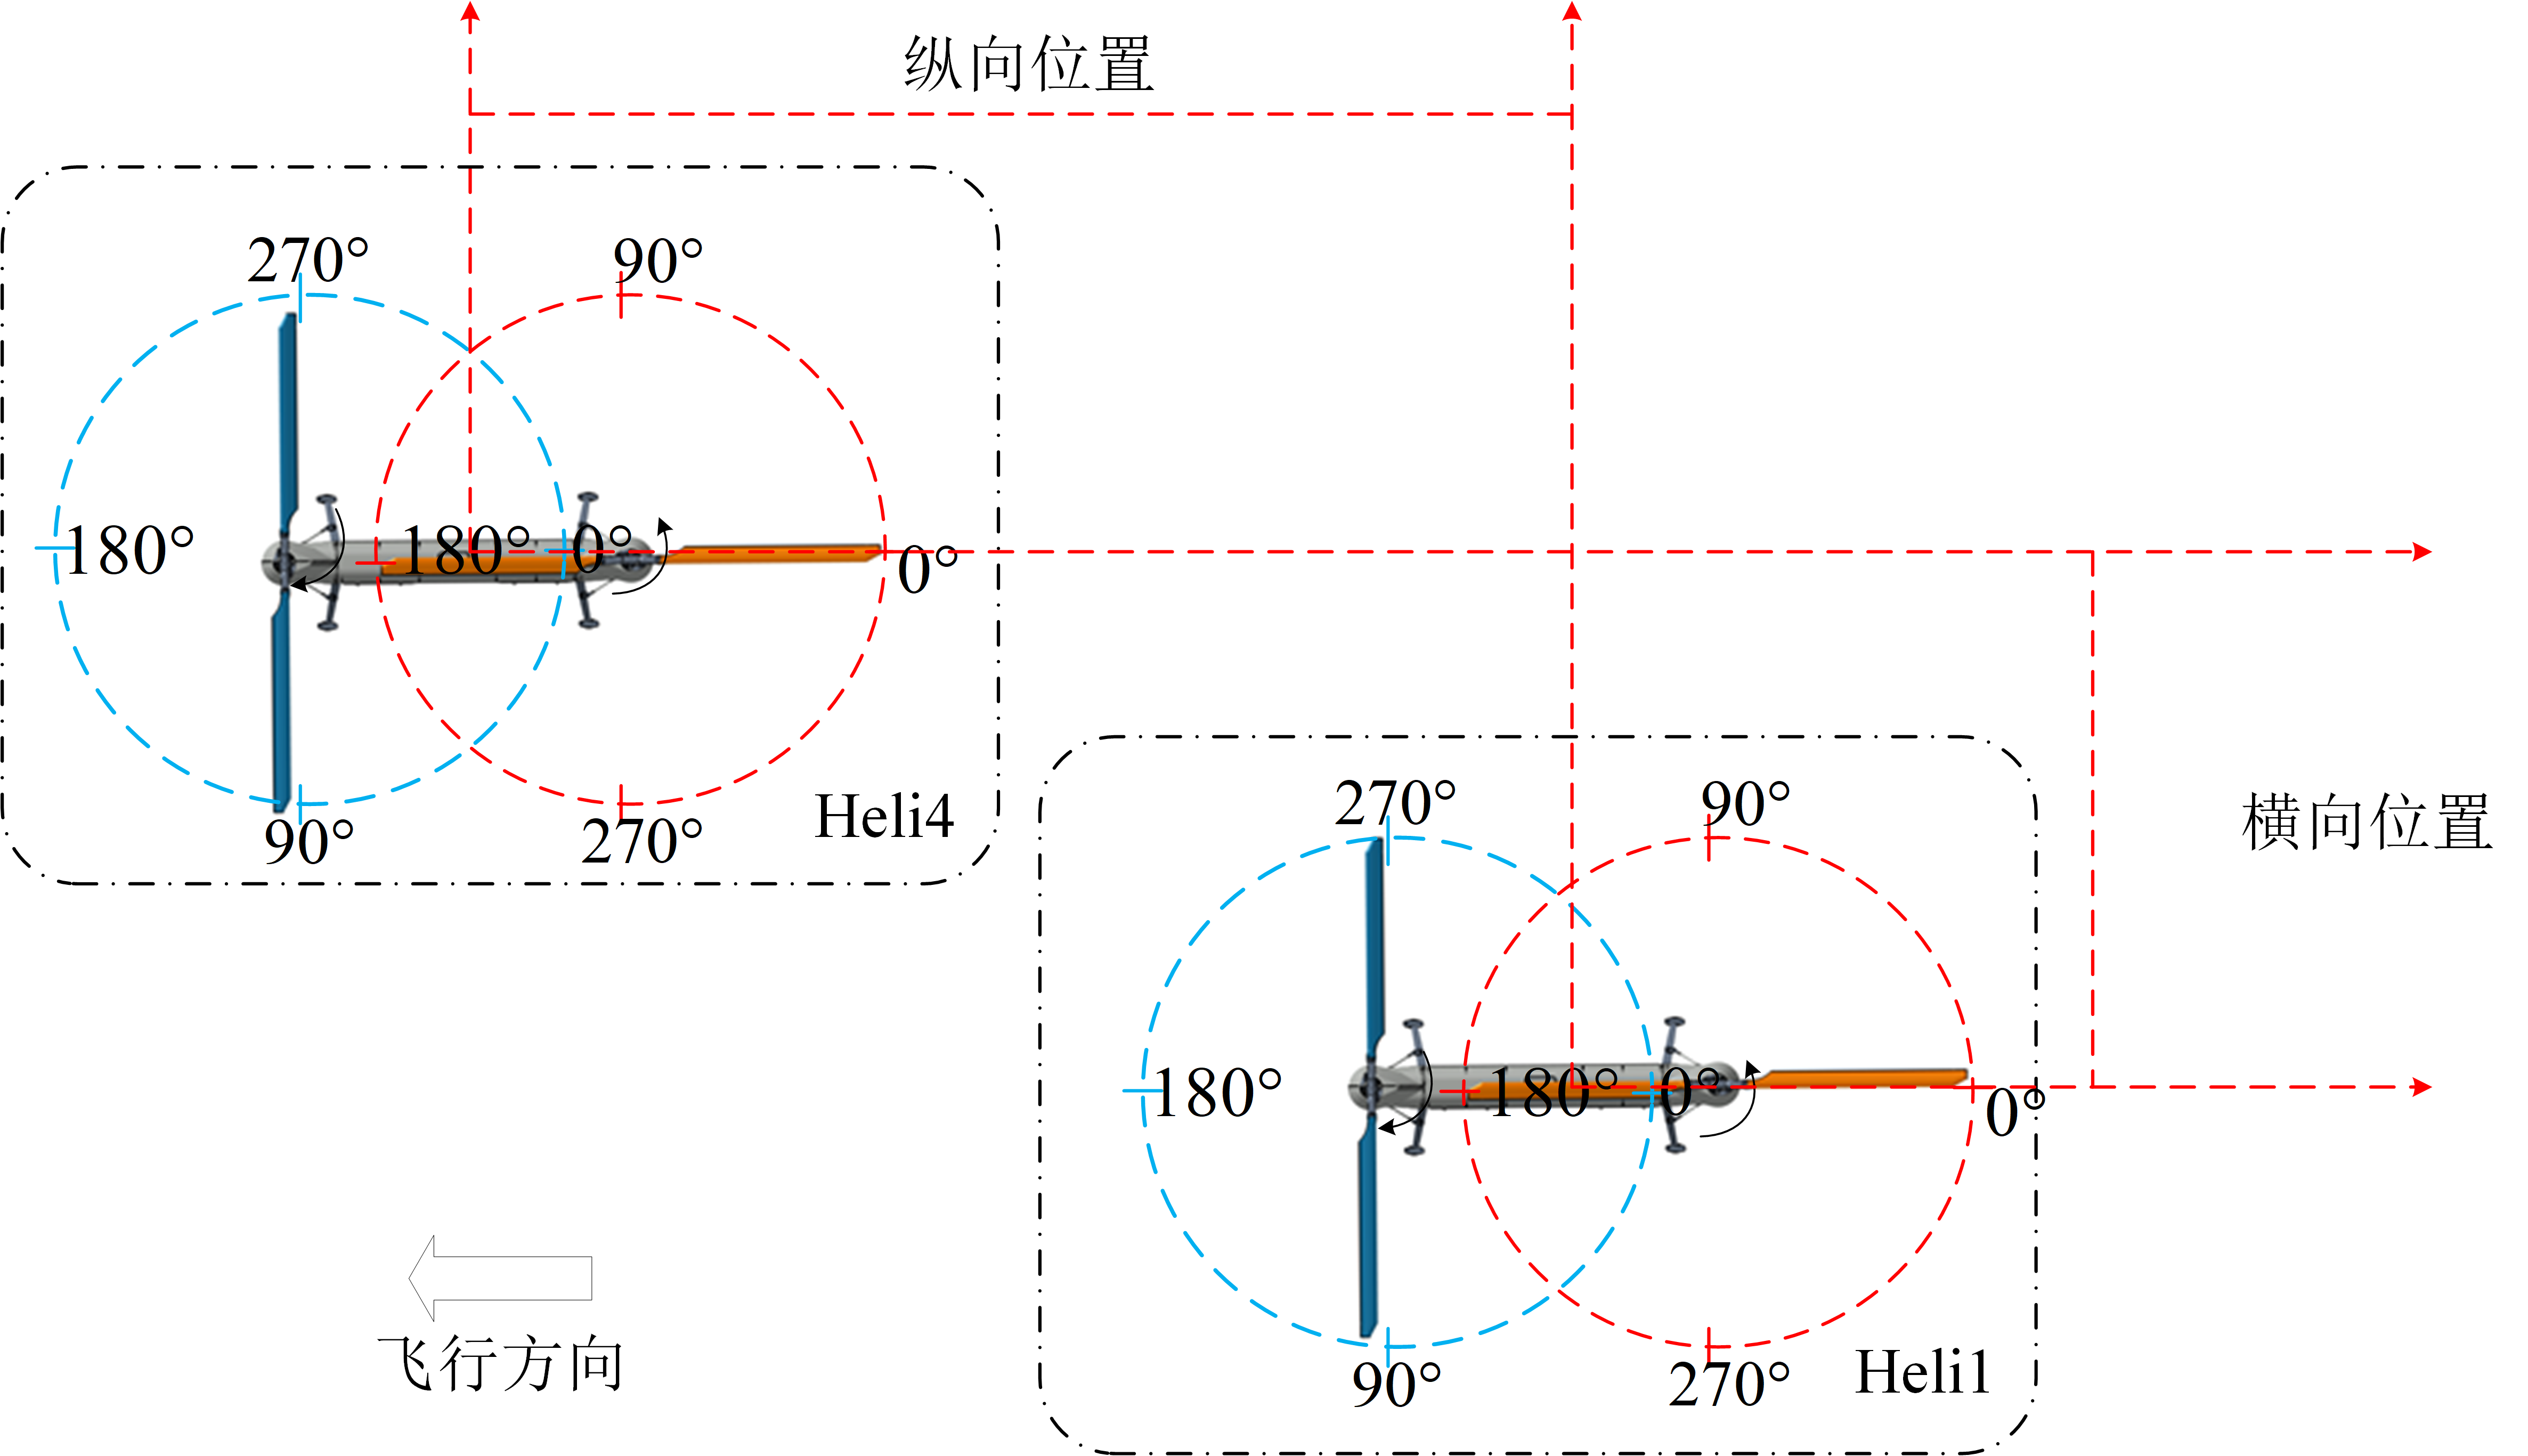
\includegraphics[width=10cm]{fig/figure_chap3/chap_3_5_1_9.png}
  \caption{直升机1和直升机4的相对位置定义\label{fig:chap3_5_1_3}}
\end{figure}
 
纵列式直升机前后旋翼的转向、直升机1与直升机4的纵向距离、直升机1与直升机4的侧向距离定义见图\ref{fig:chap3_5_1_3}。

\subsection{不同横向相对位置下气动干扰及性能的变化}
本小节给出了气动干扰随直升机横向相对位置的变化,其中直升机1相对直升机4的横向相对位置变化范围为-1.5到1.5倍的旋翼直径。相对位置为-1.5倍的旋翼直径时,表示直升机1在直升机4的左后方;相对位置为1.5倍的旋翼直径时,表示直升机1在直升机4的右后方。

图\ref{fig:chap3_5_2_1}给出了直升机协同吊挂系统三个典型横向相对位置下的涡度场。可以看出,在基本配置中,直升机1完全沉浸在直升机4的尾流中。当左移0.5倍的旋翼直径时,只有直升机1前旋翼的后行侧、后旋翼的前行侧沉浸在直升机4的尾流中。随着横向距离的进一步增加,如\ref{fig:chap3_5_2_1}(c)所示,直升机1和直升机4之间几乎没有干扰。

此外,值得一提的是,直升机1相对直升机4右移时的干扰情况与左移时类似。唯一不同的是,当右移0.5到1倍的旋翼直径时,直升机1前旋翼的前行侧、后旋翼的后行侧沉浸在直升机4的尾流中。
\begin{figure}[!htb]
  \centering
  \subfloat[基本配置]{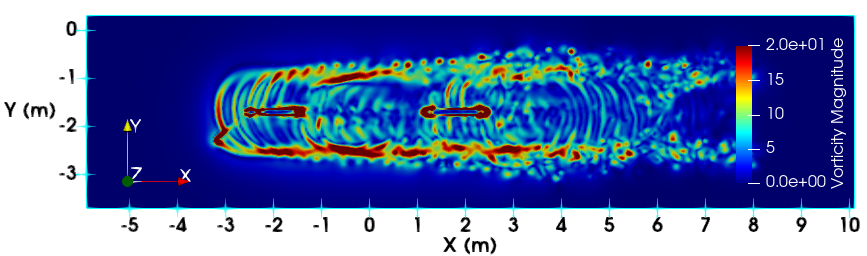
\includegraphics[width=7cm]{fig/figure_chap3/chap_3_5_2_1.png}}\\ 
  \subfloat[左移0.5倍旋翼直径]{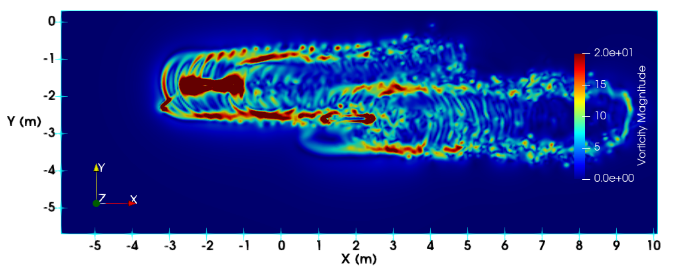
\includegraphics[width=7cm]{fig/figure_chap3/chap_3_5_2_2.png}}\quad
  \subfloat[左移一倍旋翼直径]{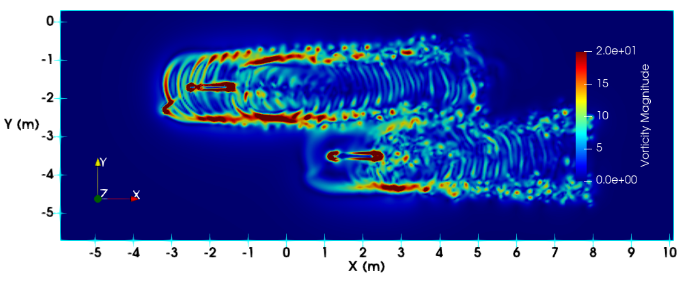
\includegraphics[width=7cm]{fig/figure_chap3/chap_3_5_2_3.png}}
  \caption{直升机协同吊挂系统不同横向相对位置下的涡度场}
  \label{fig:chap3_5_2_1}
\end{figure}

图\ref{fig:chap3_5_2_2}(a)给出了直升机1前旋翼0.75R处的截面力。可以看出,基本配置、左移0.5倍旋翼直升机、左移1倍旋翼直径三种情况下,方位角100 \degree 到 250 \degree 期间,截面力有较大差距。基本配置中,直升机1完全沉浸在直升机4的尾流中,所以截面力远远比其他两种情况下小。左移0.5倍的旋翼直径时,方位角200 \degree 到 250 \degree 间的截面力远远小于方位角100 \degree 到 170 \degree 间的截面力。左移1倍的旋翼直径时,各个方位角的力均比其他两种情况下大。上述变化与不同相对侧向位置下的气动干扰变化相一致。

此外,根据图\ref{fig:chap3_5_2_2}(b)直升机1后旋翼0.75R处的截面力可知,相对侧向位置对直升机1后旋翼的影响较小。这是由于直升机1后旋翼受到前旋翼尾流的影响远远比受到直升机4的尾流影响大。

\begin{figure}[!htb]
  \centering
  \subfloat[前旋翼]{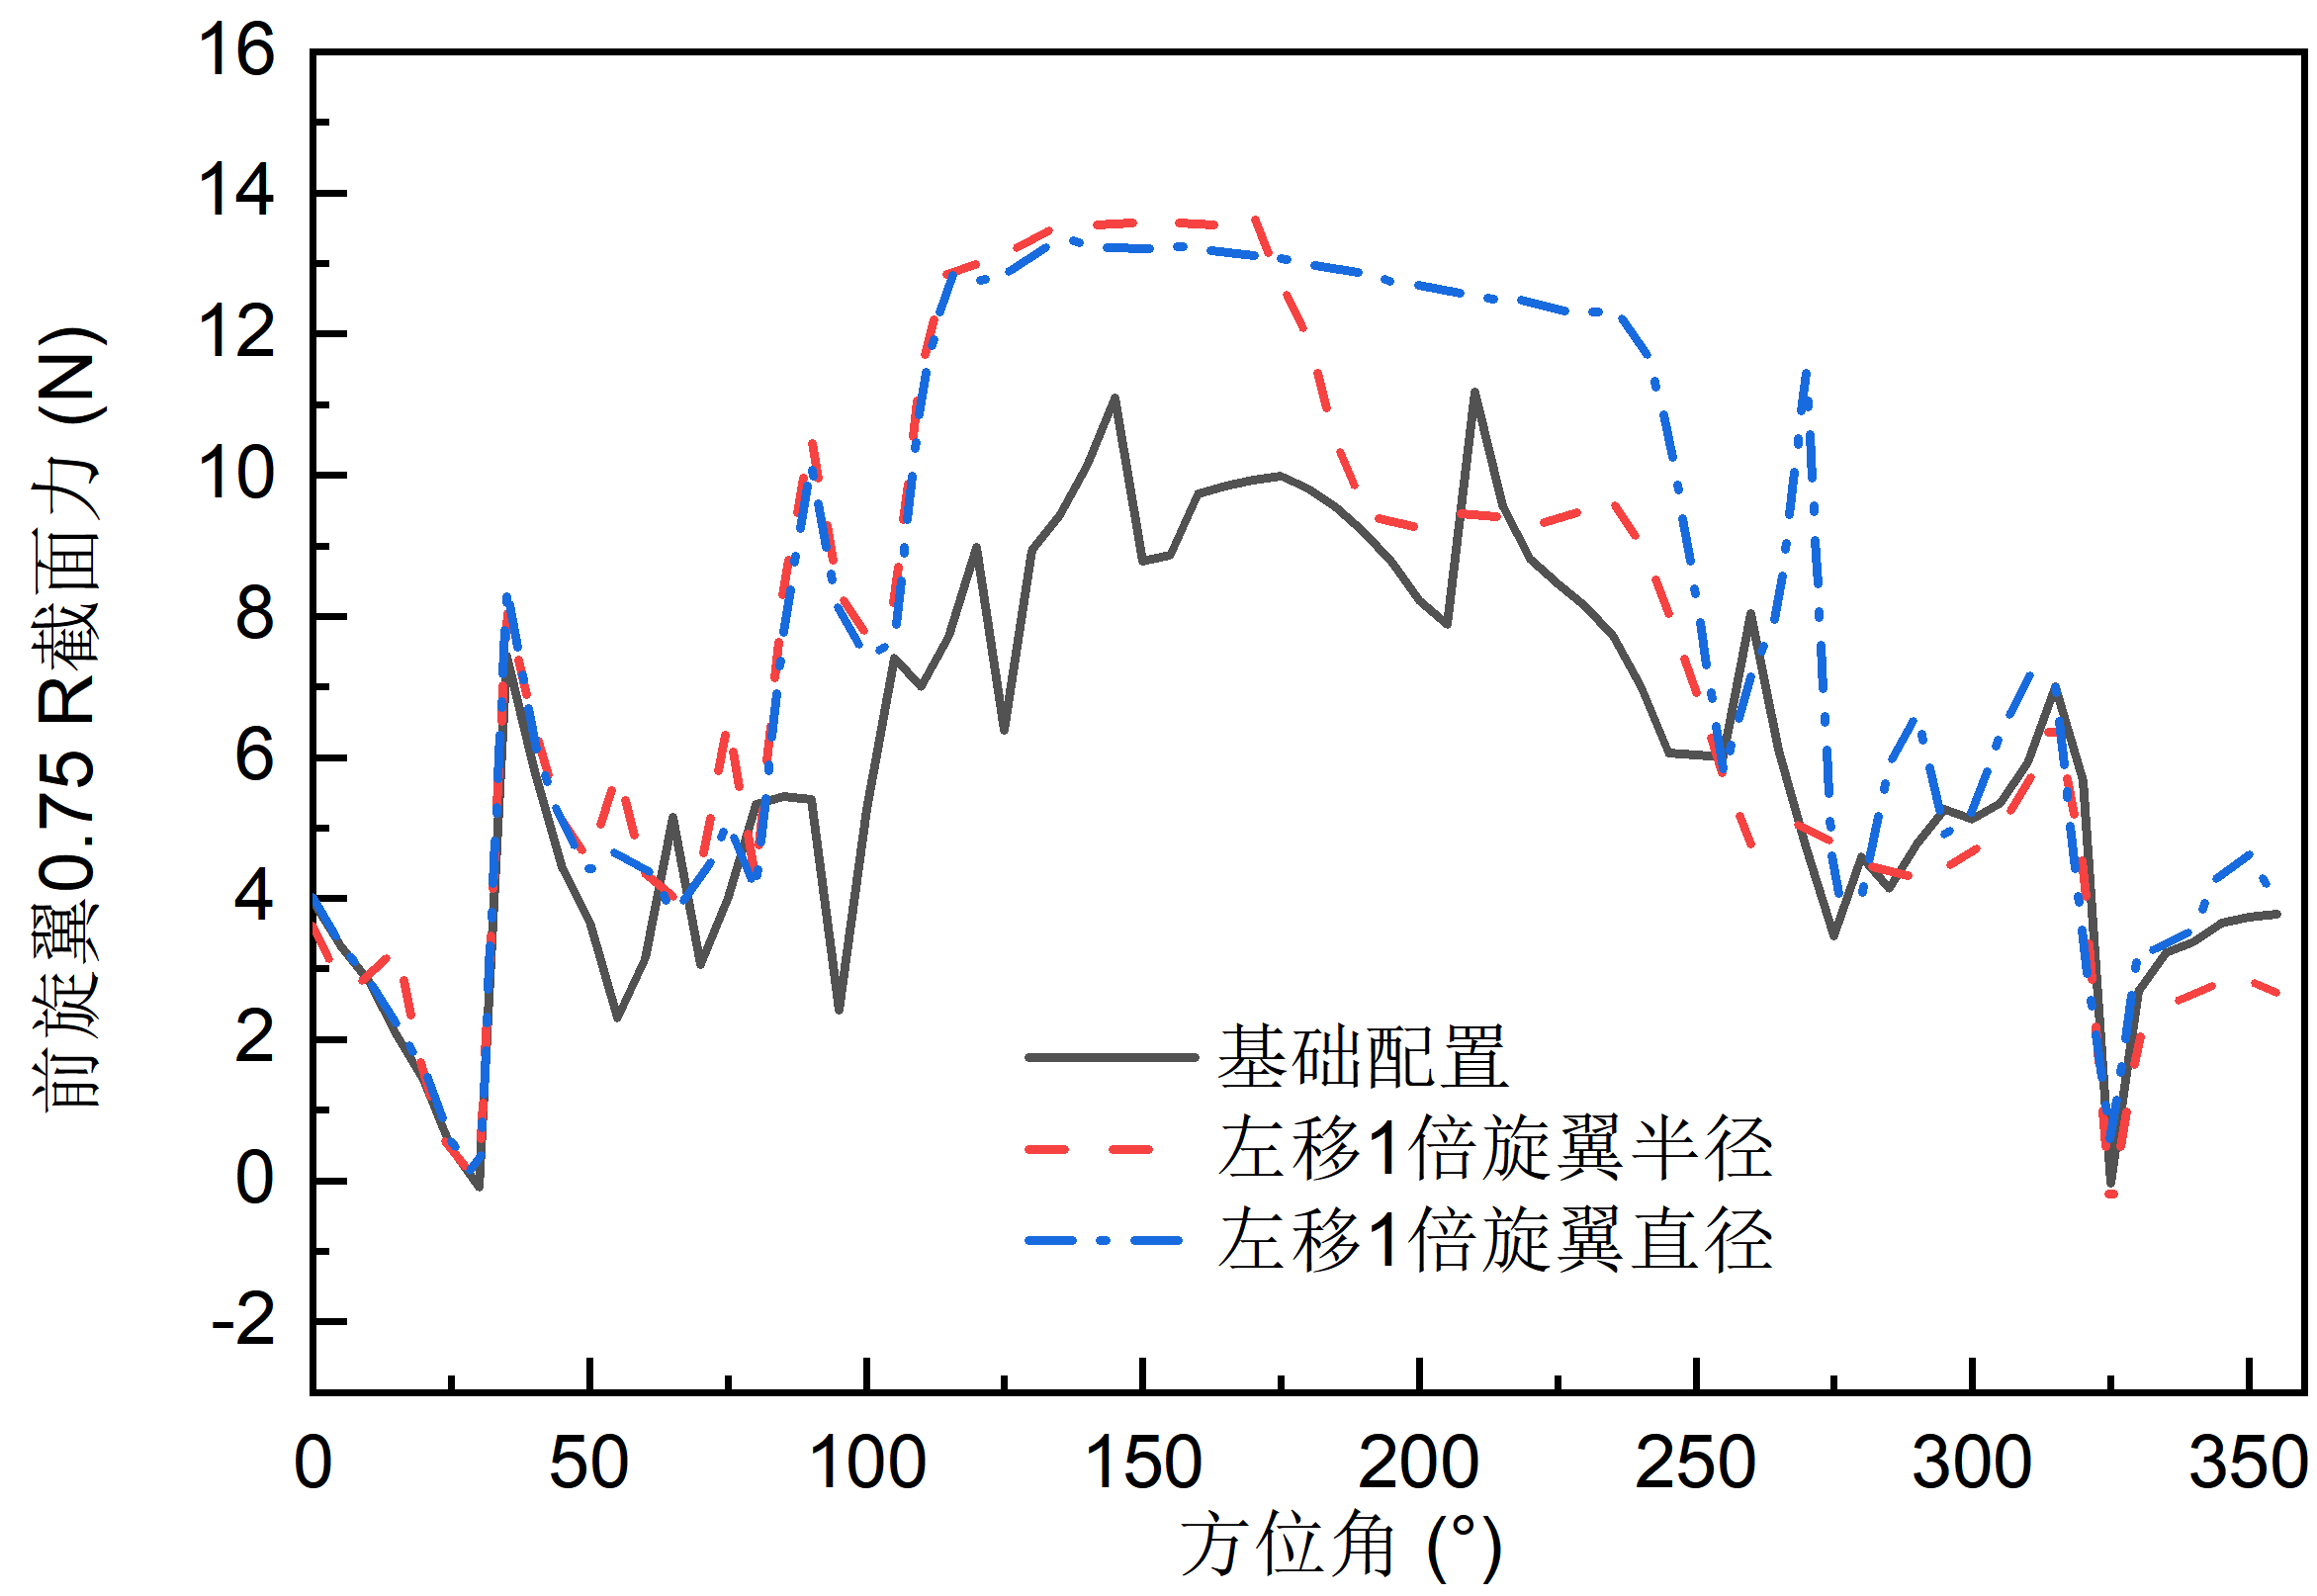
\includegraphics[width=7cm]{fig/figure_chap3/chap_3_5_2_4.png}}\quad
  \subfloat[后旋翼]{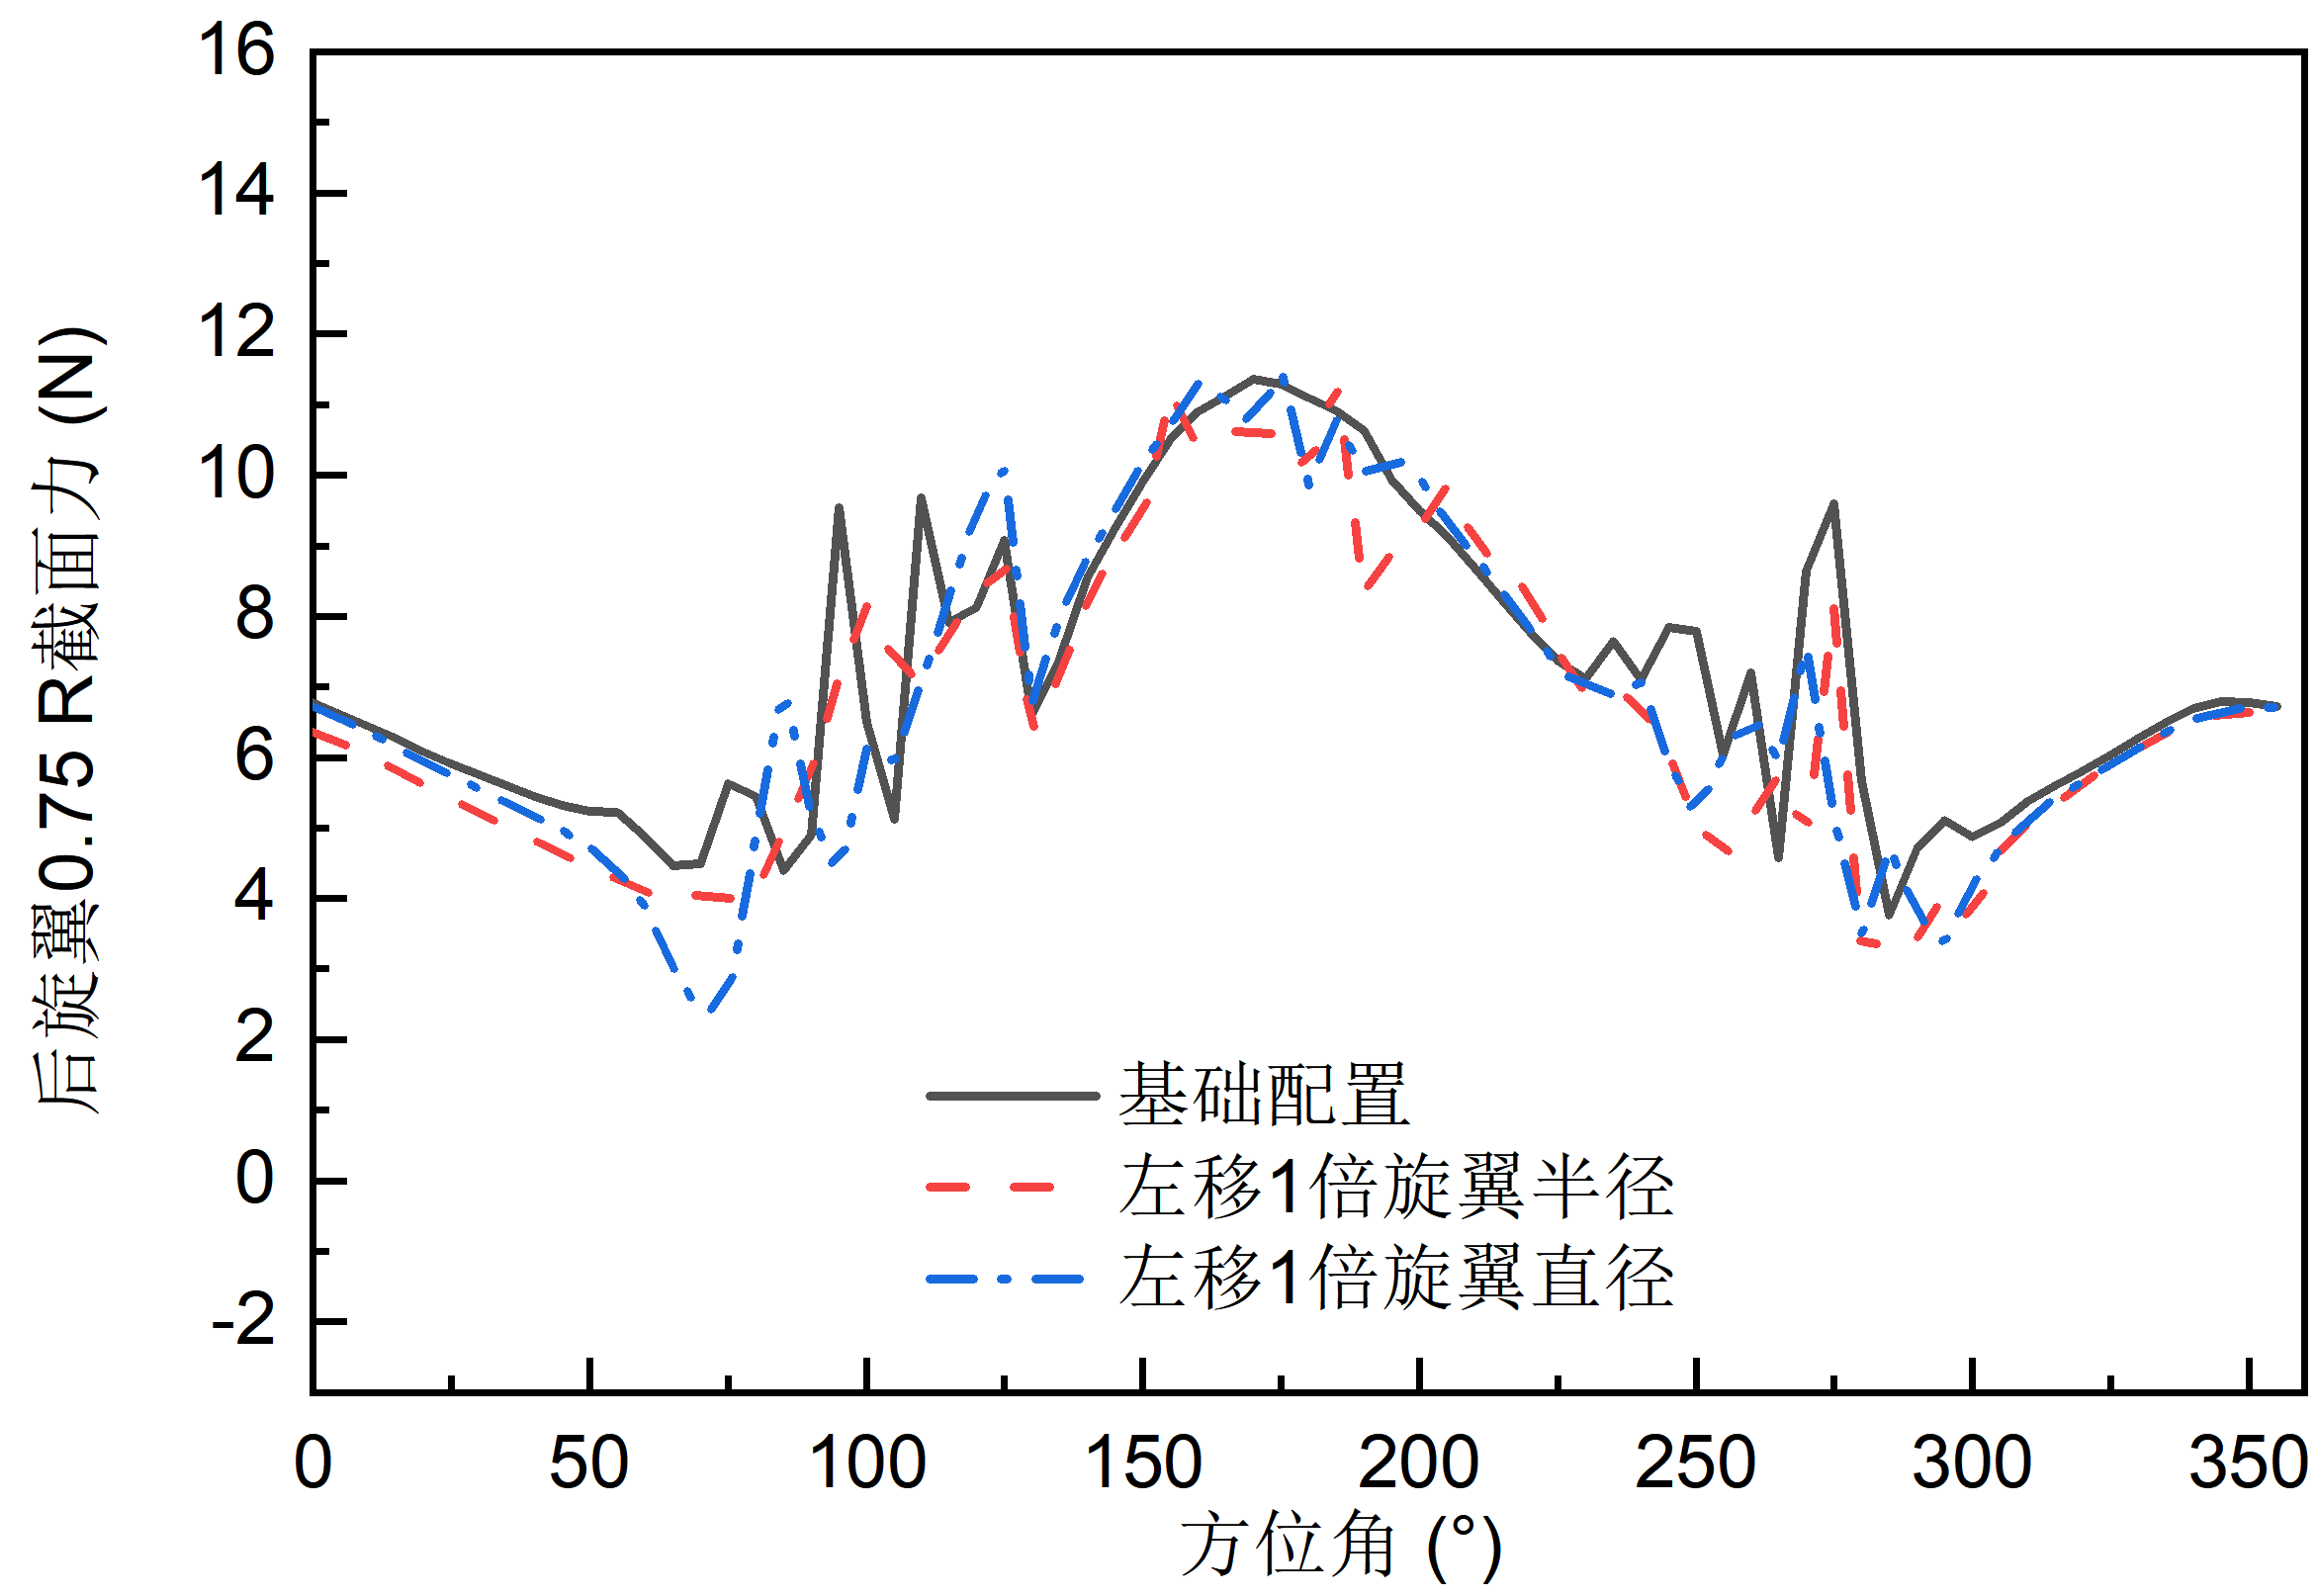
\includegraphics[width=7cm]{fig/figure_chap3/chap_3_5_2_5.png}}
  \caption{不同侧向相对位置下0.75 R 处的截面力}
  \label{fig:chap3_5_2_2}
\end{figure}

图\ref{fig:chap3_5_2_3}给出不同侧向相对位置下直升机1拉力和功率的变化。其中,100\%的前旋翼拉力对应95 N;100\%的后旋翼拉力对应83 N。100\%的前旋翼功率对应310 W;100\%的后旋翼功率对应452 W。这些值是直升机1不受直升机4的气动干扰影响时计算得到的。基本配置中,即相对侧向位置等于0时,前旋翼有20\%的拉力损失和15\%的功耗增加。随着侧向相对位置正向、负向增加,拉力增加、功耗减小。当侧向相对位置处于-1.5到-0.75倍的旋翼直径、0.75到1.5倍的旋翼直径时,相比无干扰时,拉力增加、功率减小。这得益于较小的下洗流干扰和卷起涡引起的迎角增加。此外,后旋翼拉力和功率的变化较小。这与横向相对位置变化时,后旋翼0.75 R 截面拉力的变化规律是一致的。

\begin{figure}[!htb]
  \centering
  \subfloat[拉力变化]{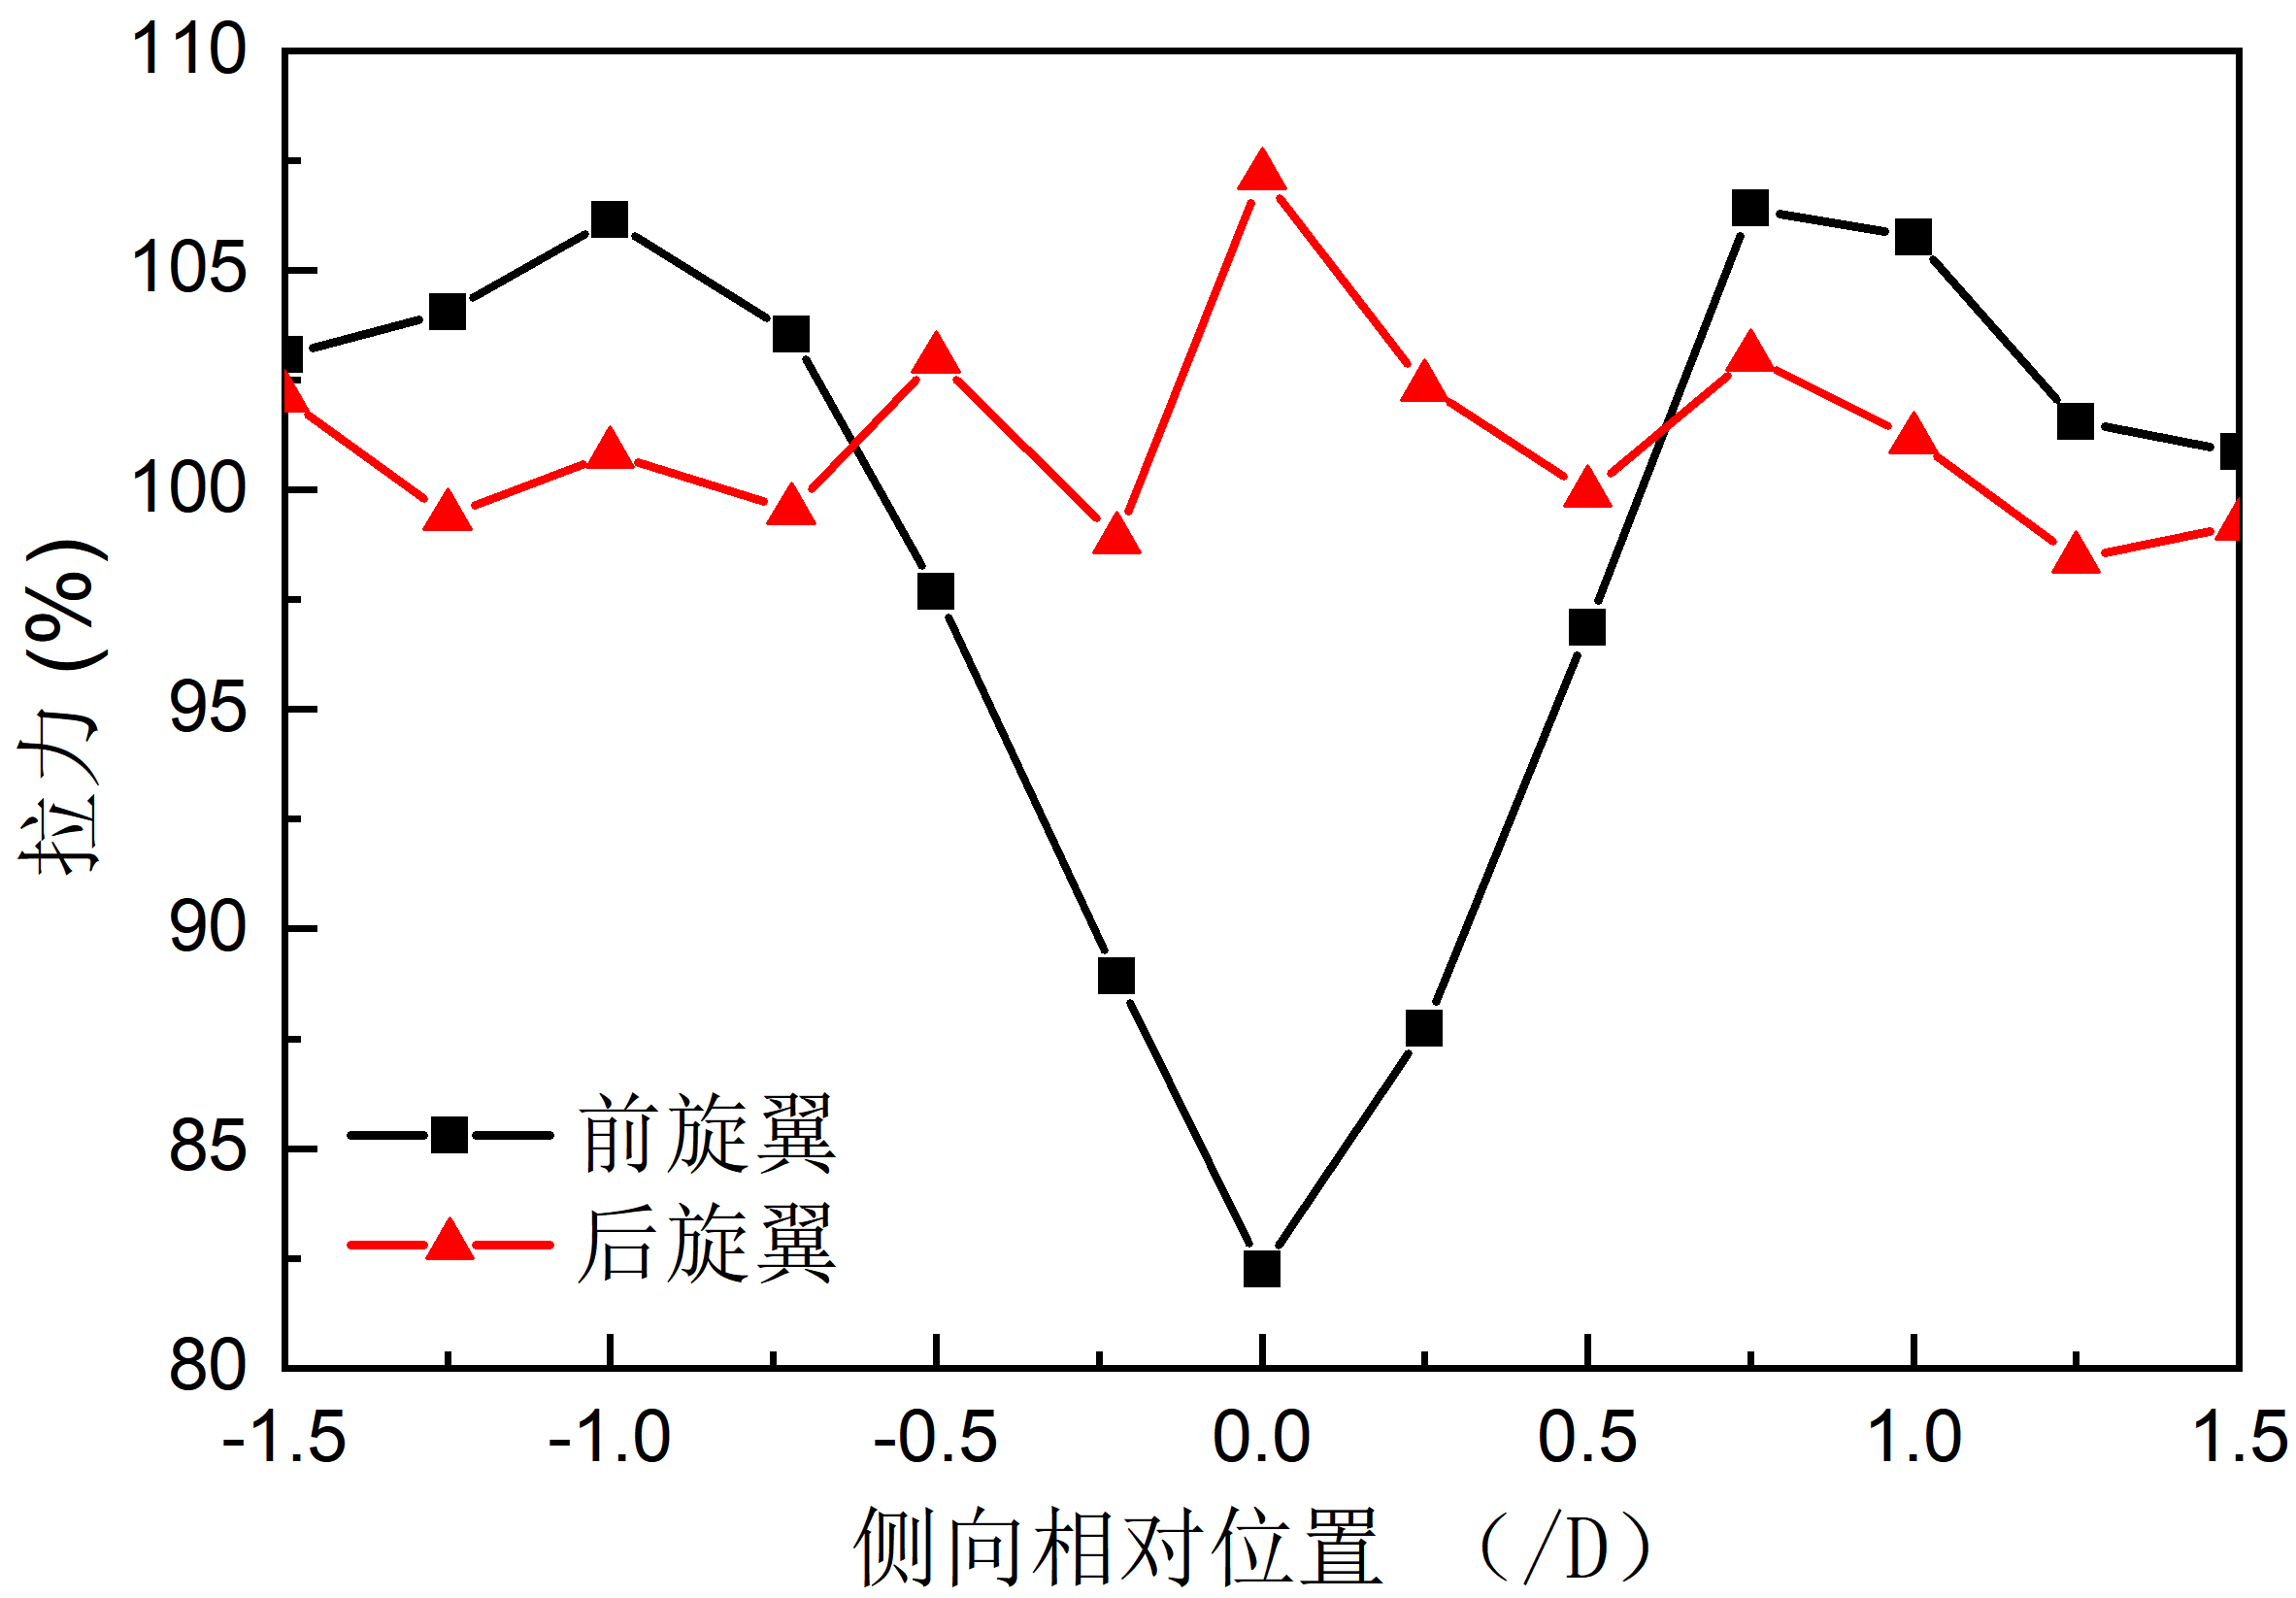
\includegraphics[width=7cm]{fig/figure_chap3/chap_3_5_2_6.png}}\quad 
  \subfloat[功率变化]{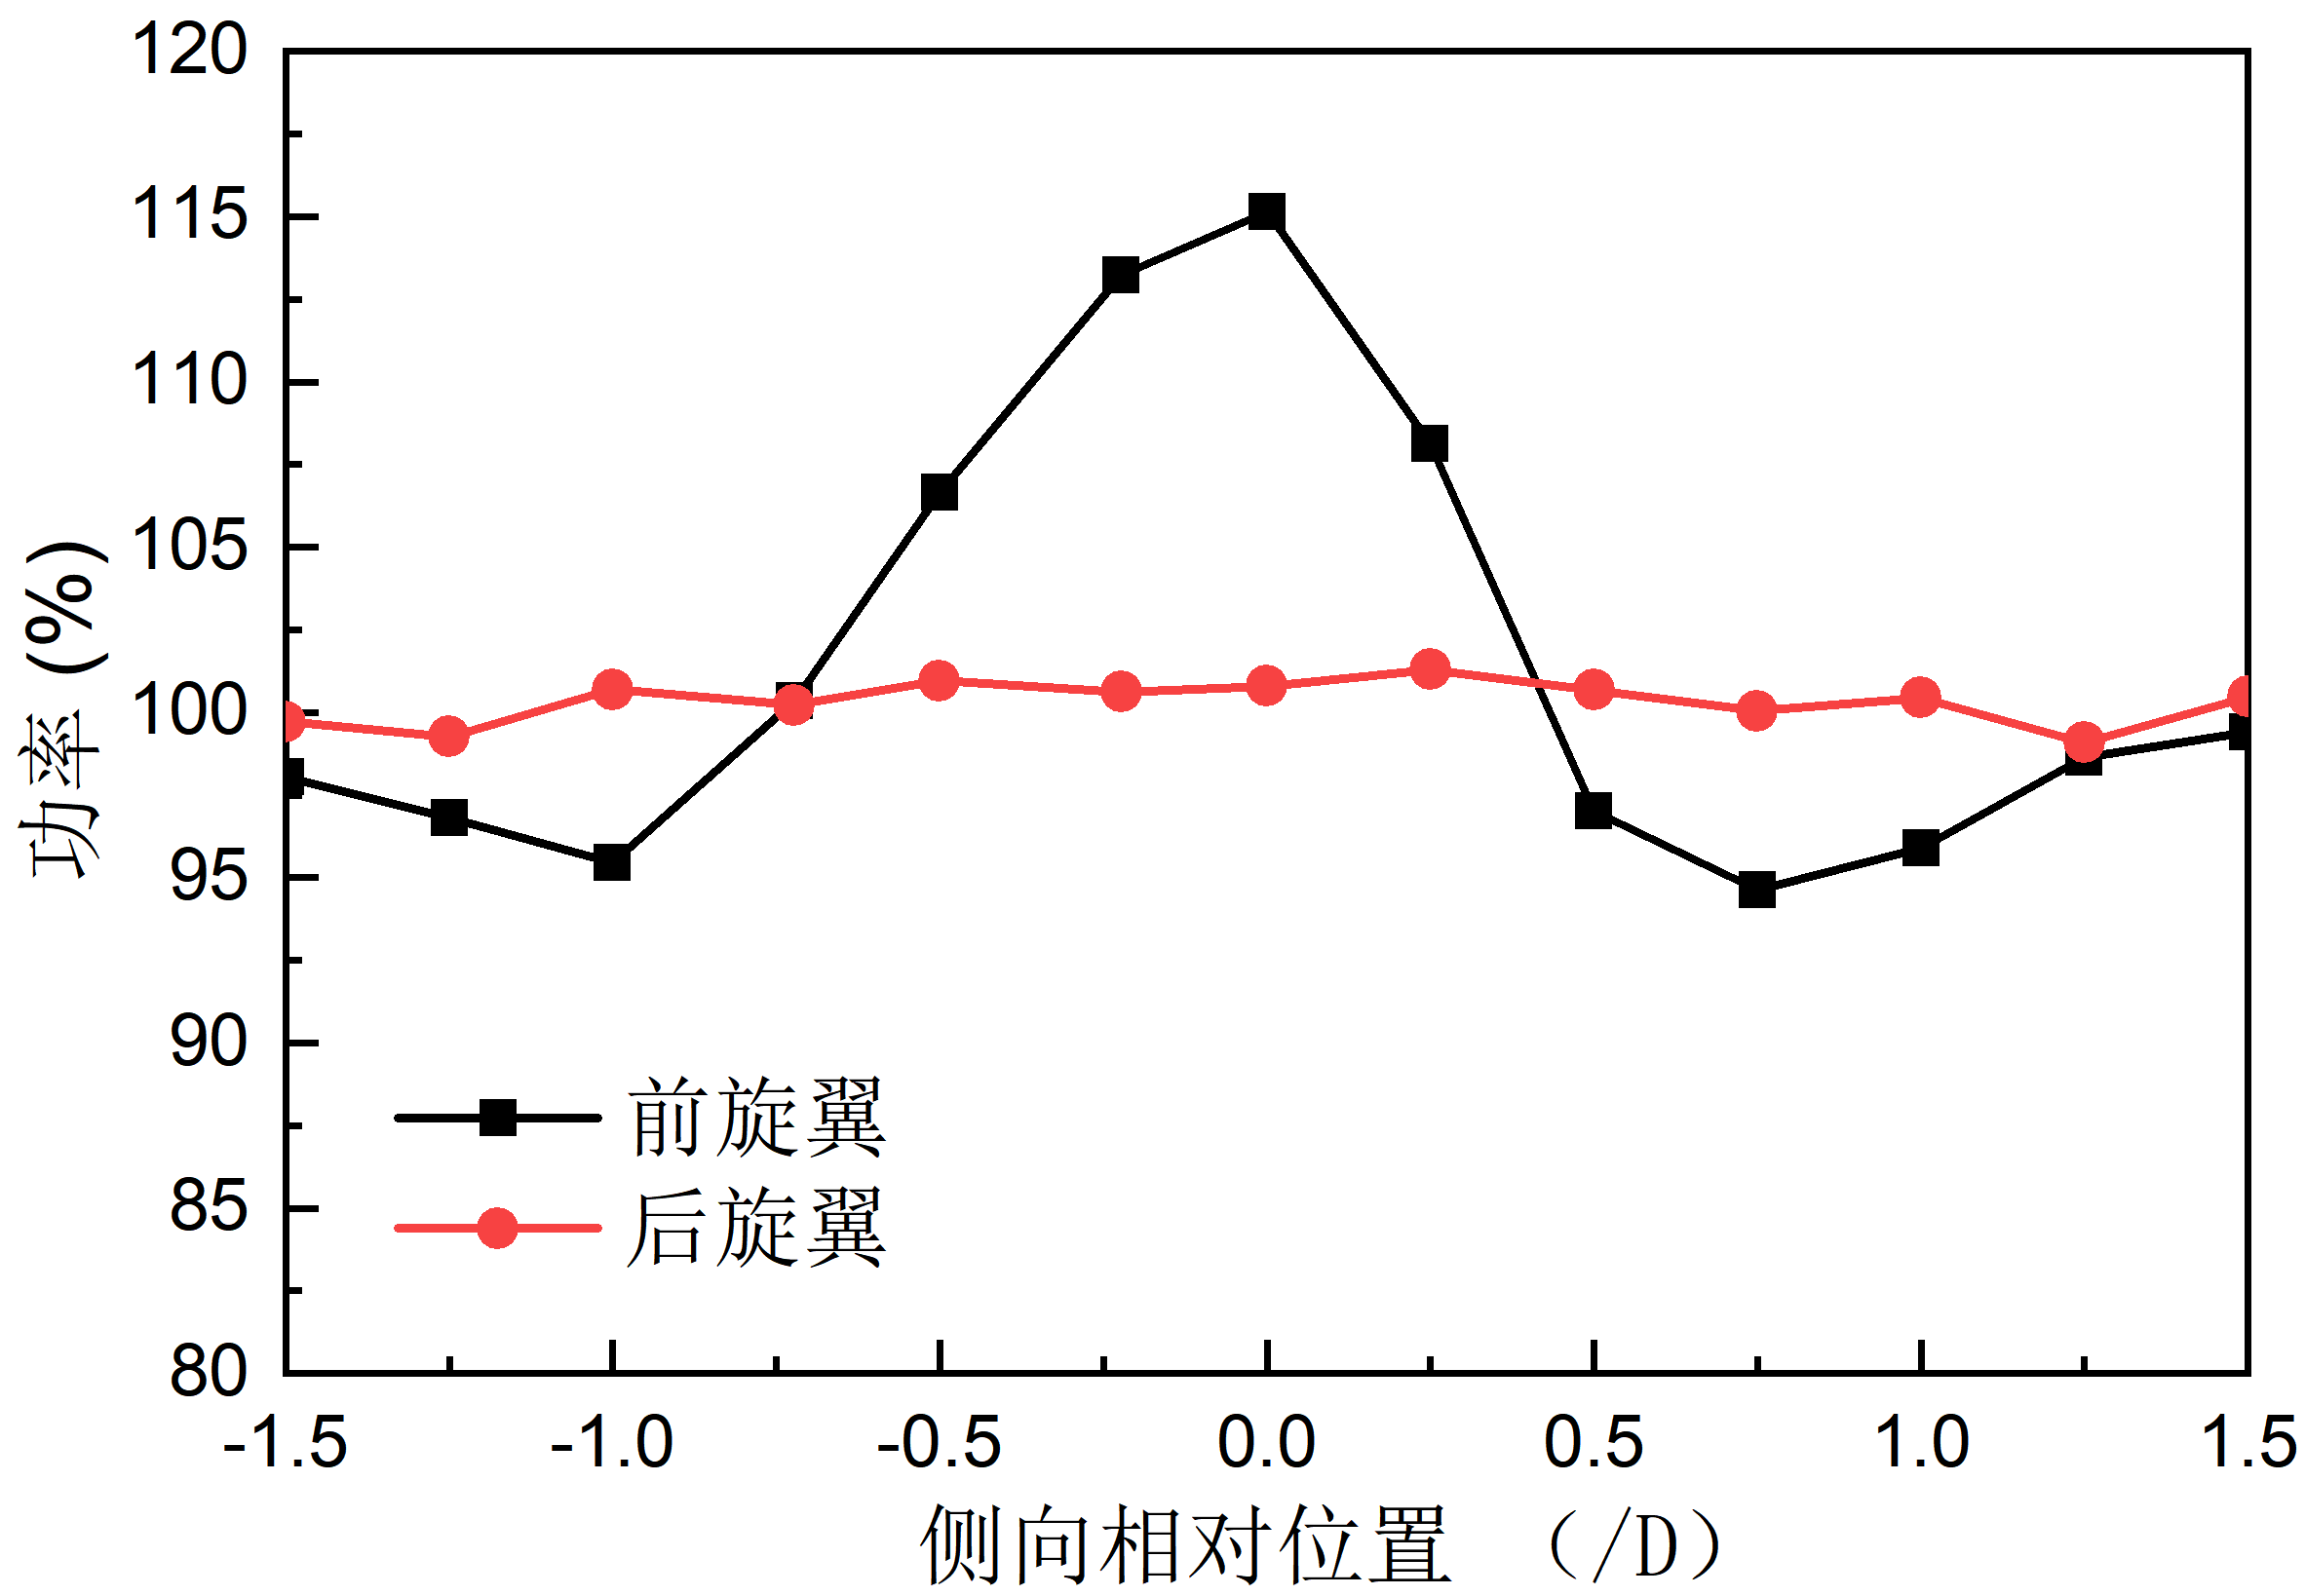
\includegraphics[width=7cm]{fig/figure_chap3/chap_3_5_2_7.png}}
  \caption{不同侧向相对位置下直升机1拉力和功率的变化}
  \label{fig:chap3_5_2_3}
\end{figure}

可见,基本配置中,由于气动干扰的影响直升机1有一定的拉力损失和功耗增加。通过合理调整直升机1相对直升机4的侧向位置,拉力损失和功率都会减小。甚至当侧向相对位置处于-1.5到-0.75倍的旋翼直径、0.75到1.5倍的旋翼直径时,相对无干扰时拉力增加、功效减小。
\subsection{不同纵向相对位置下气动干扰及性能的变化}
本小节给出了气动干扰随直升机纵向相对位置的变化。图\ref{fig:chap3_5_3_1}给出了直升机1相对基本配置前进、后退1个旋翼半径时的涡度场。与基本配置中的涡度场(见图\ref{fig:chap3_5_2_1}(a))相比可以发现,气动干扰随着直升机1和直升机4间距离的减小而增加。
\begin{figure}[!htb]
  \centering
  \subfloat[直升机1向前1个旋翼半径]{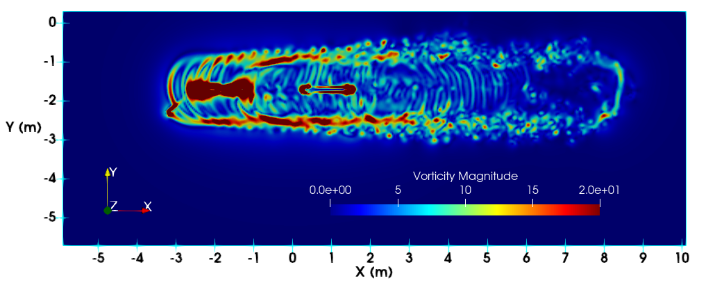
\includegraphics[width=7cm]{fig/figure_chap3/chap_3_5_3_1.png}}\quad 
  \subfloat[直升机1向后1个旋翼半径]{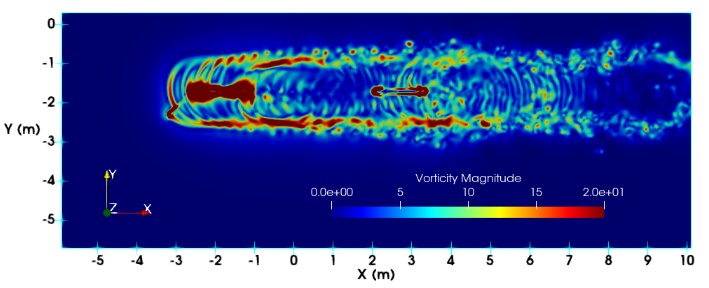
\includegraphics[width=7cm]{fig/figure_chap3/chap_3_5_3_2.png}}
  \caption{直升机协同吊挂系统不同纵向相对位置下的涡度场}
  \label{fig:chap3_5_3_1}
\end{figure}

图\ref{fig:chap3_5_3_2}给出了前后旋翼不同纵向相对位置下0.75 R 处的截面力。从图\ref{fig:chap3_5_3_2}(a)可以看出,多数方位角下直升机1后退1倍旋翼半径时其前旋翼的截面力均大于其他两种情况。这与上面提到的气动干扰的变化一致。与不同侧向相对位置时的结果相似,三种情况下后旋翼截面力的变化较小。这也导致了后旋翼合力、功率变化较小,分别见图\ref{fig:chap3_5_3_3}(b)和图\ref{fig:chap3_5_3_4}(b)。
\begin{figure}[!htb]
  \centering
  \subfloat[前旋翼]{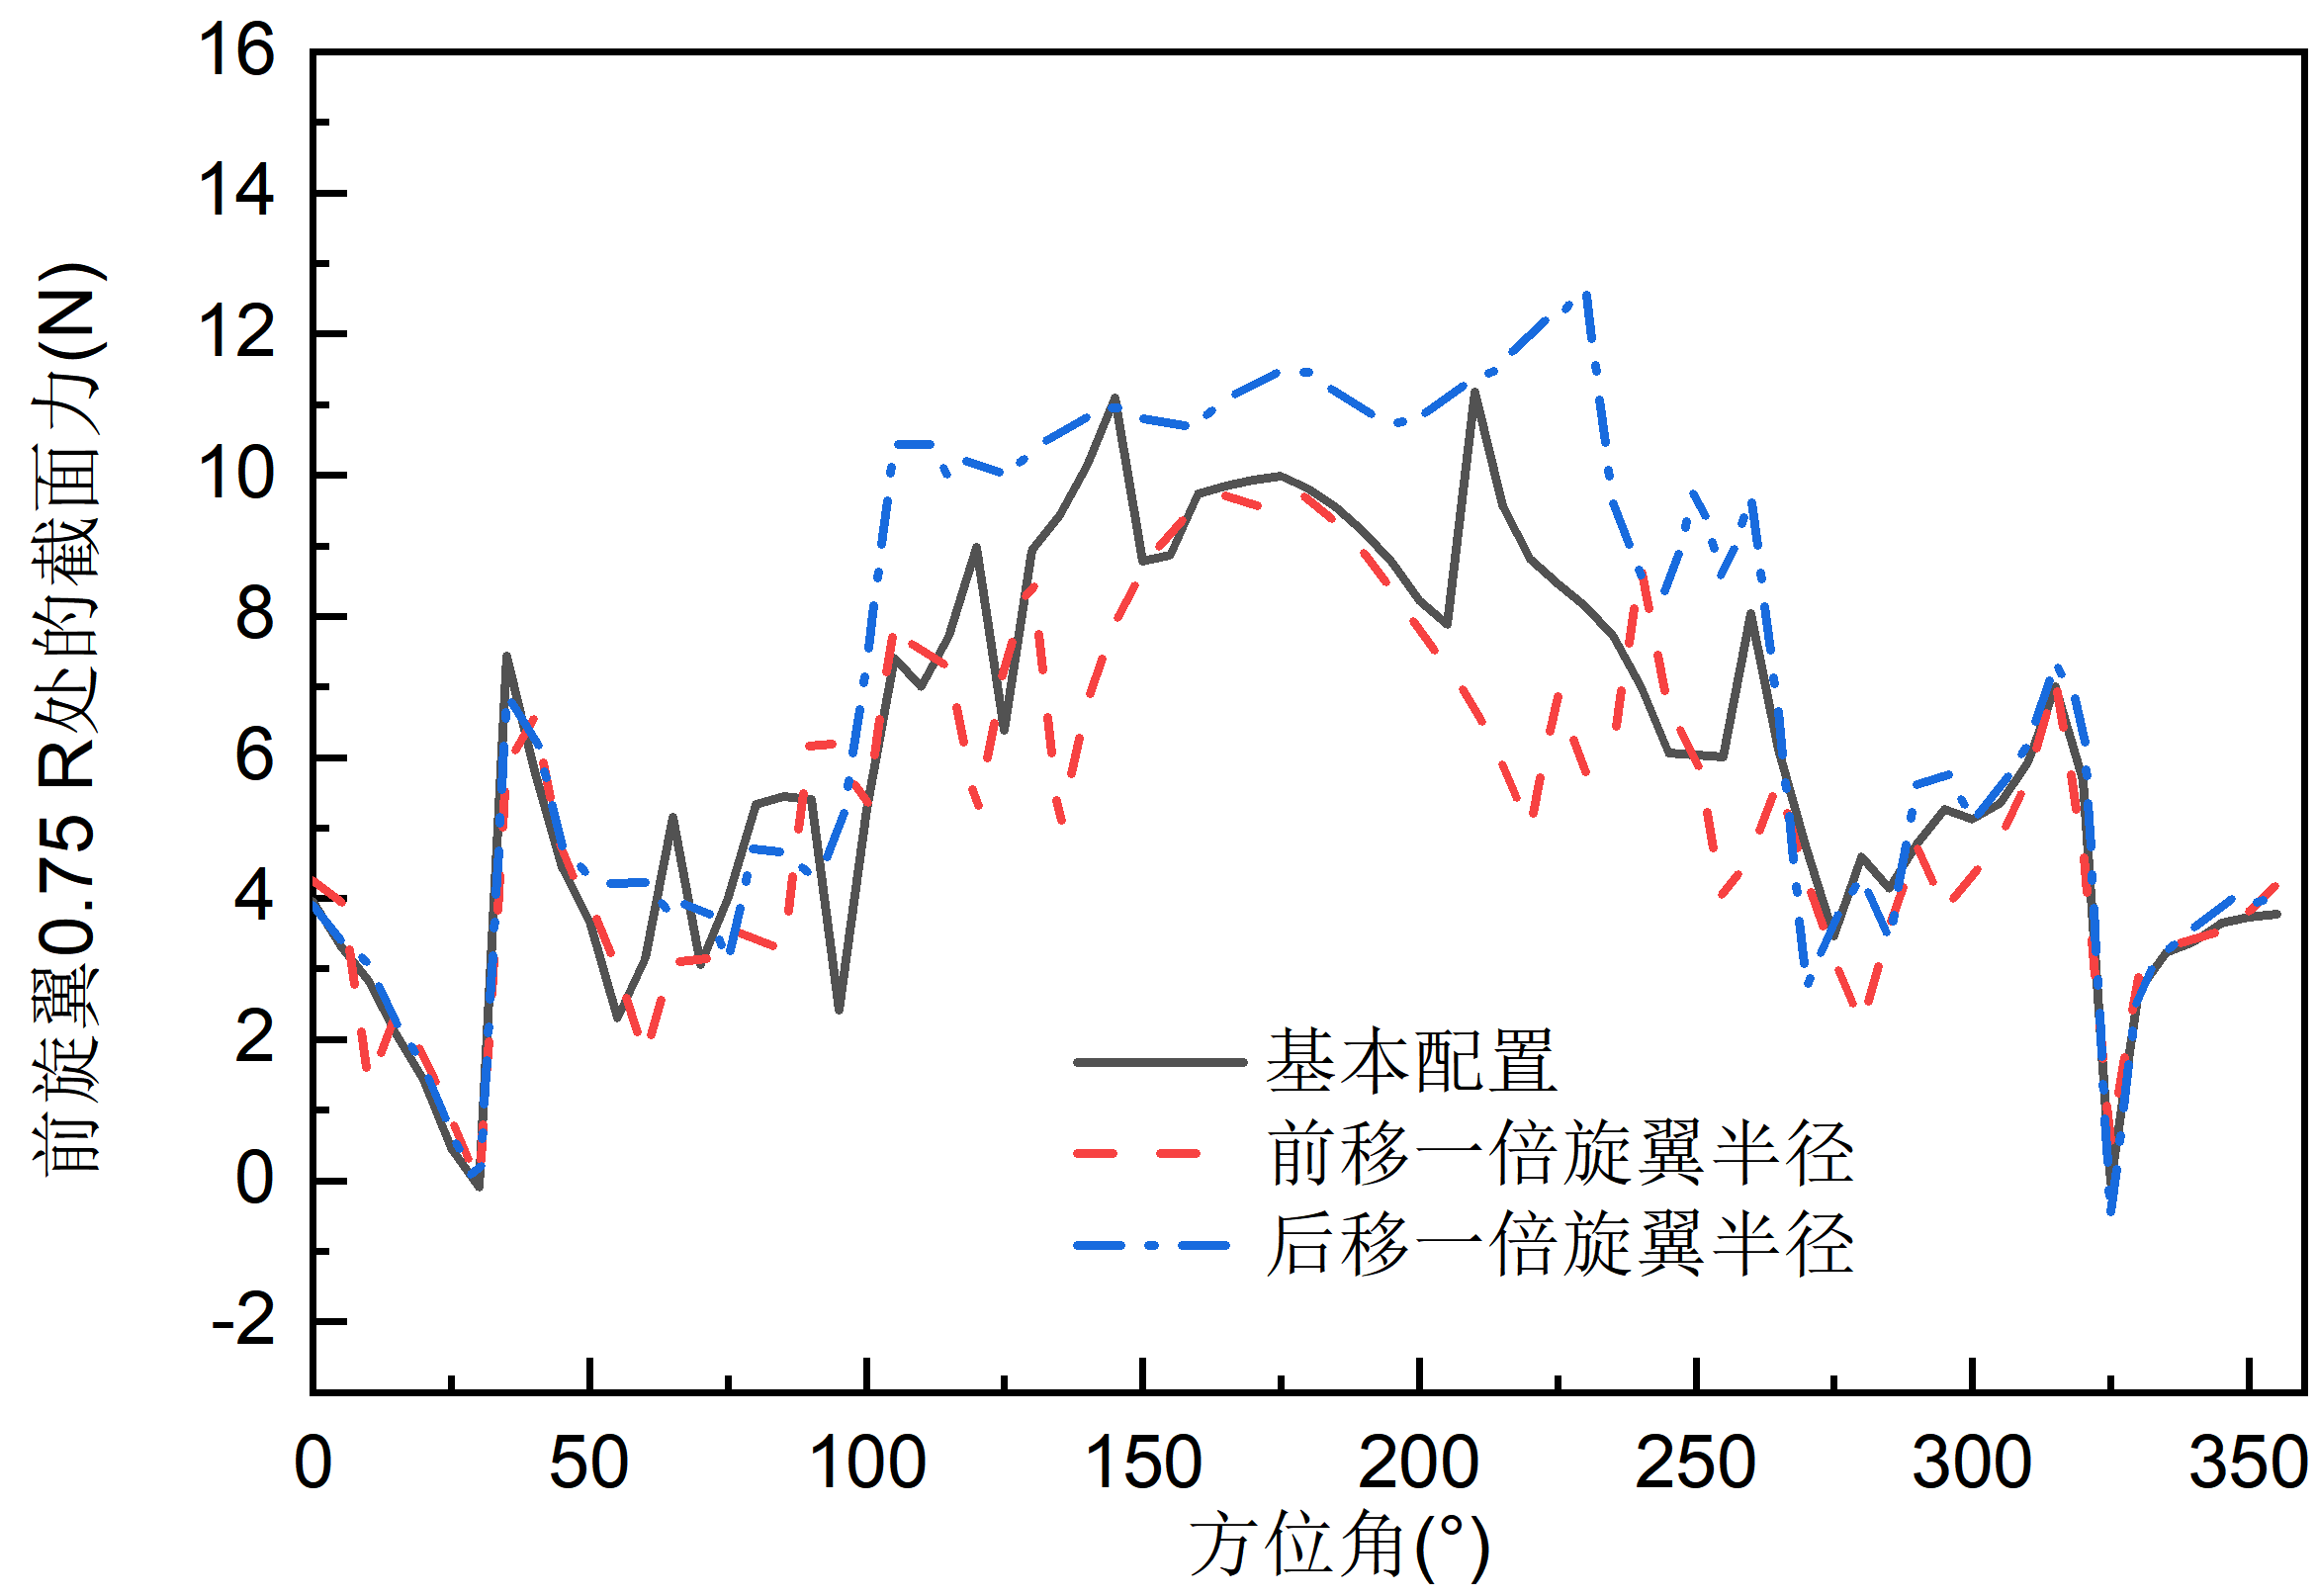
\includegraphics[width=7cm]{fig/figure_chap3/chap_3_5_3_3.png}}\quad
  \subfloat[后旋翼]{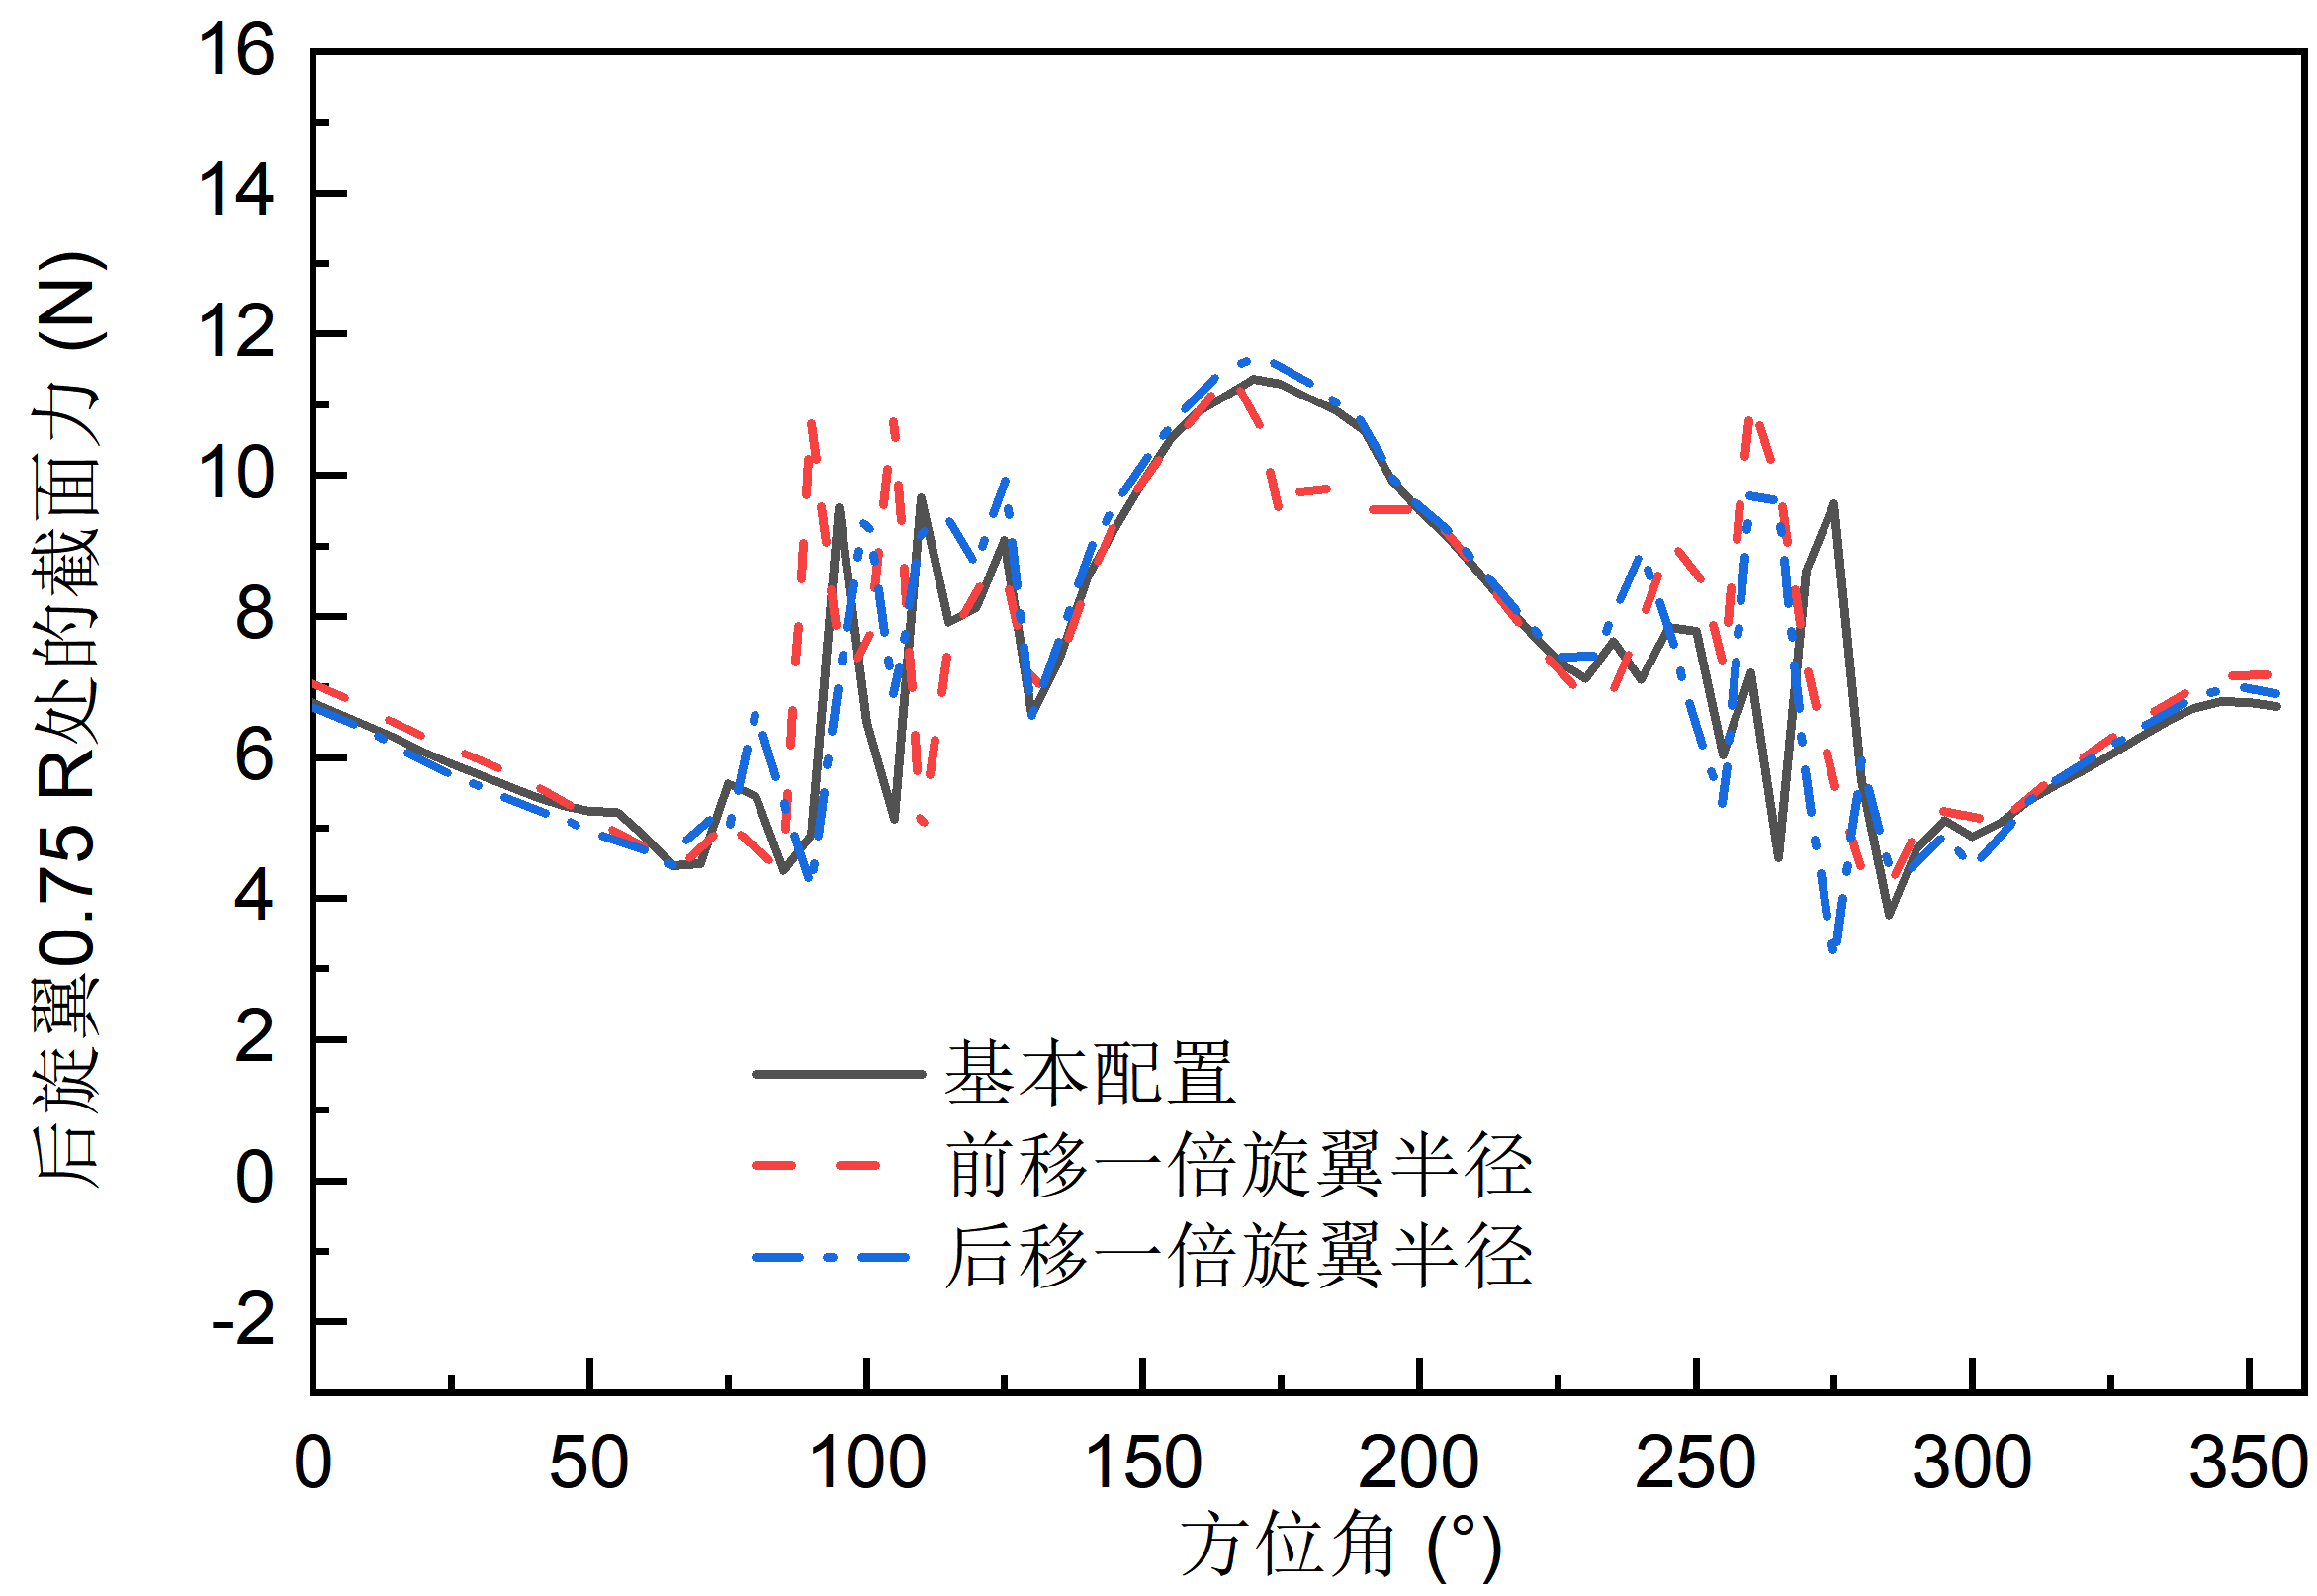
\includegraphics[width=7cm]{fig/figure_chap3/chap_3_5_3_4.png}}
  \caption{不同纵向相对位置下0.75 R 处的截面力}
  \label{fig:chap3_5_3_2}
\end{figure}

图\ref{fig:chap3_5_3_3}(a)和图\ref{fig:chap3_5_3_4}(a)给出了不同纵向相对位置下前旋翼拉力和功率的变化。可以看出,当侧向相对位置处于-1到1倍的旋翼半径时,拉力损失和功率消耗随着直升机1和直升机4间纵向相对位置的增加而减小。当侧向相对位置处于-1.5倍旋翼直径到-1倍旋翼半径、1倍旋翼半径到1.5倍旋翼直径时,拉力损失和功率消耗随着纵向相对距离的增加而增加。这是由于纵向相对距离越小,由上卷涡引起的作用在叶片上的上洗气流越大。

\begin{figure}[!htb]
  \centering
  \subfloat[前旋翼]{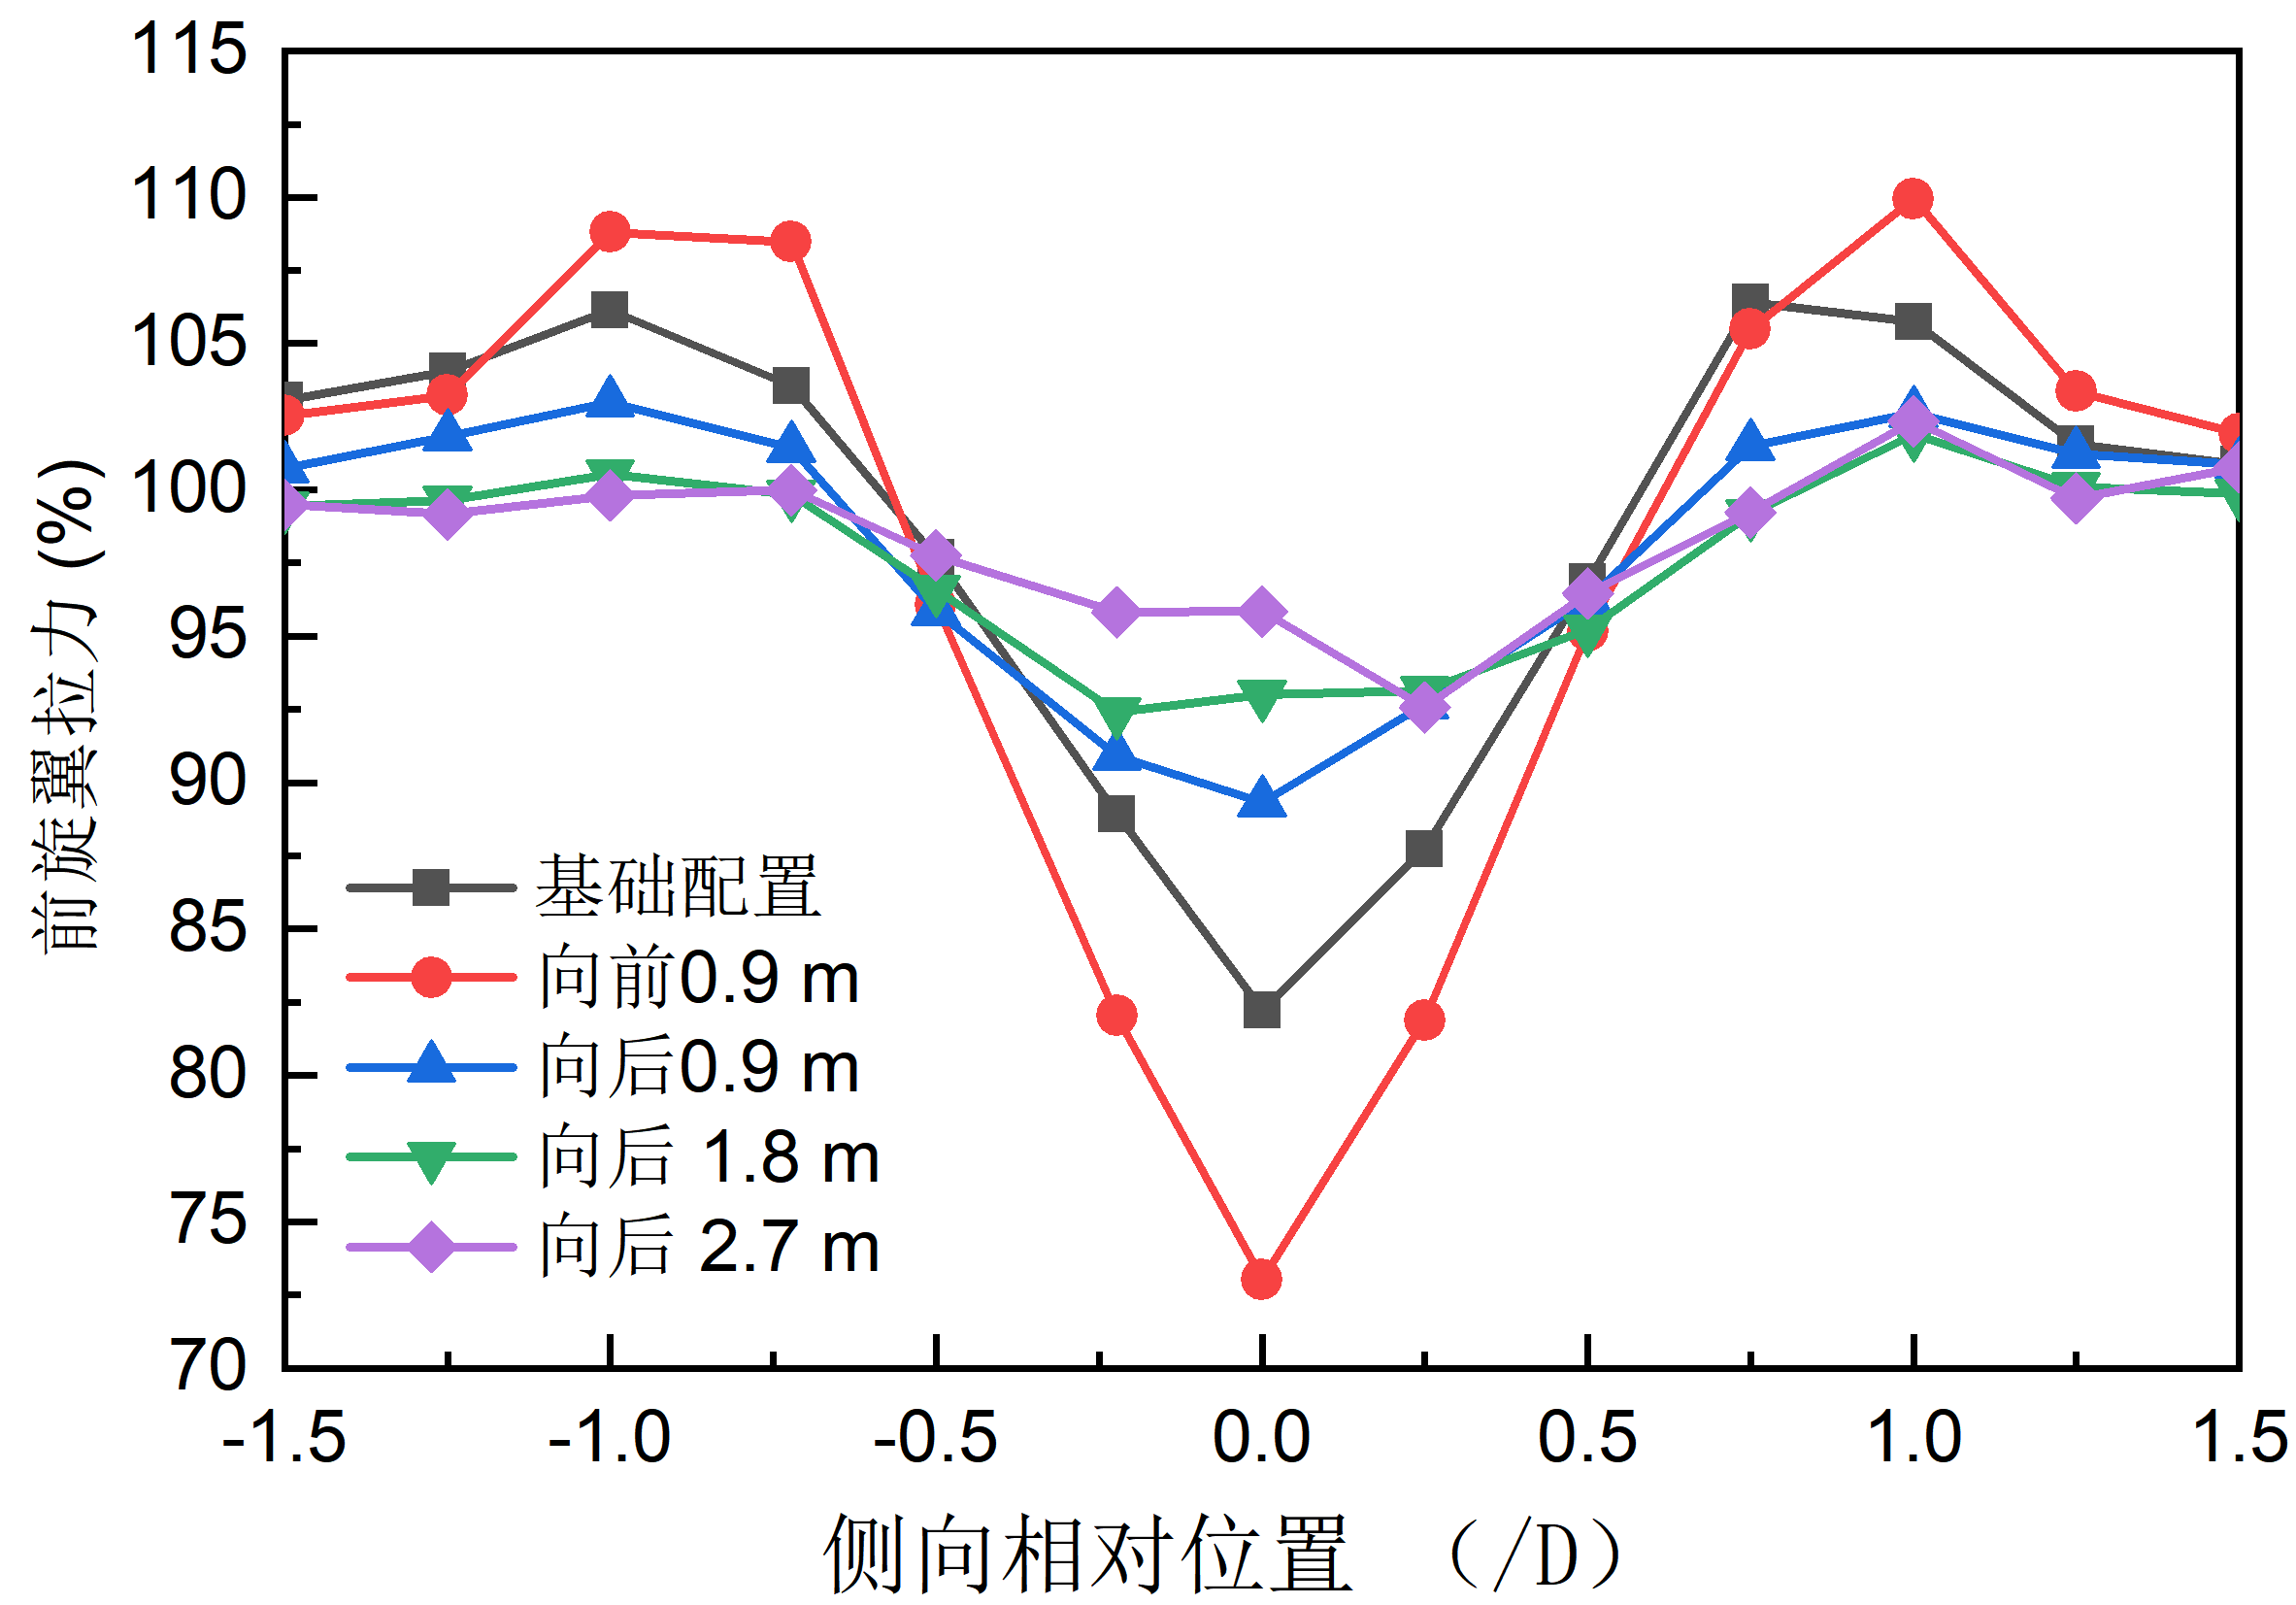
\includegraphics[width=7cm]{fig/figure_chap3/chap_3_5_3_5.png}}\quad
  \subfloat[后旋翼]{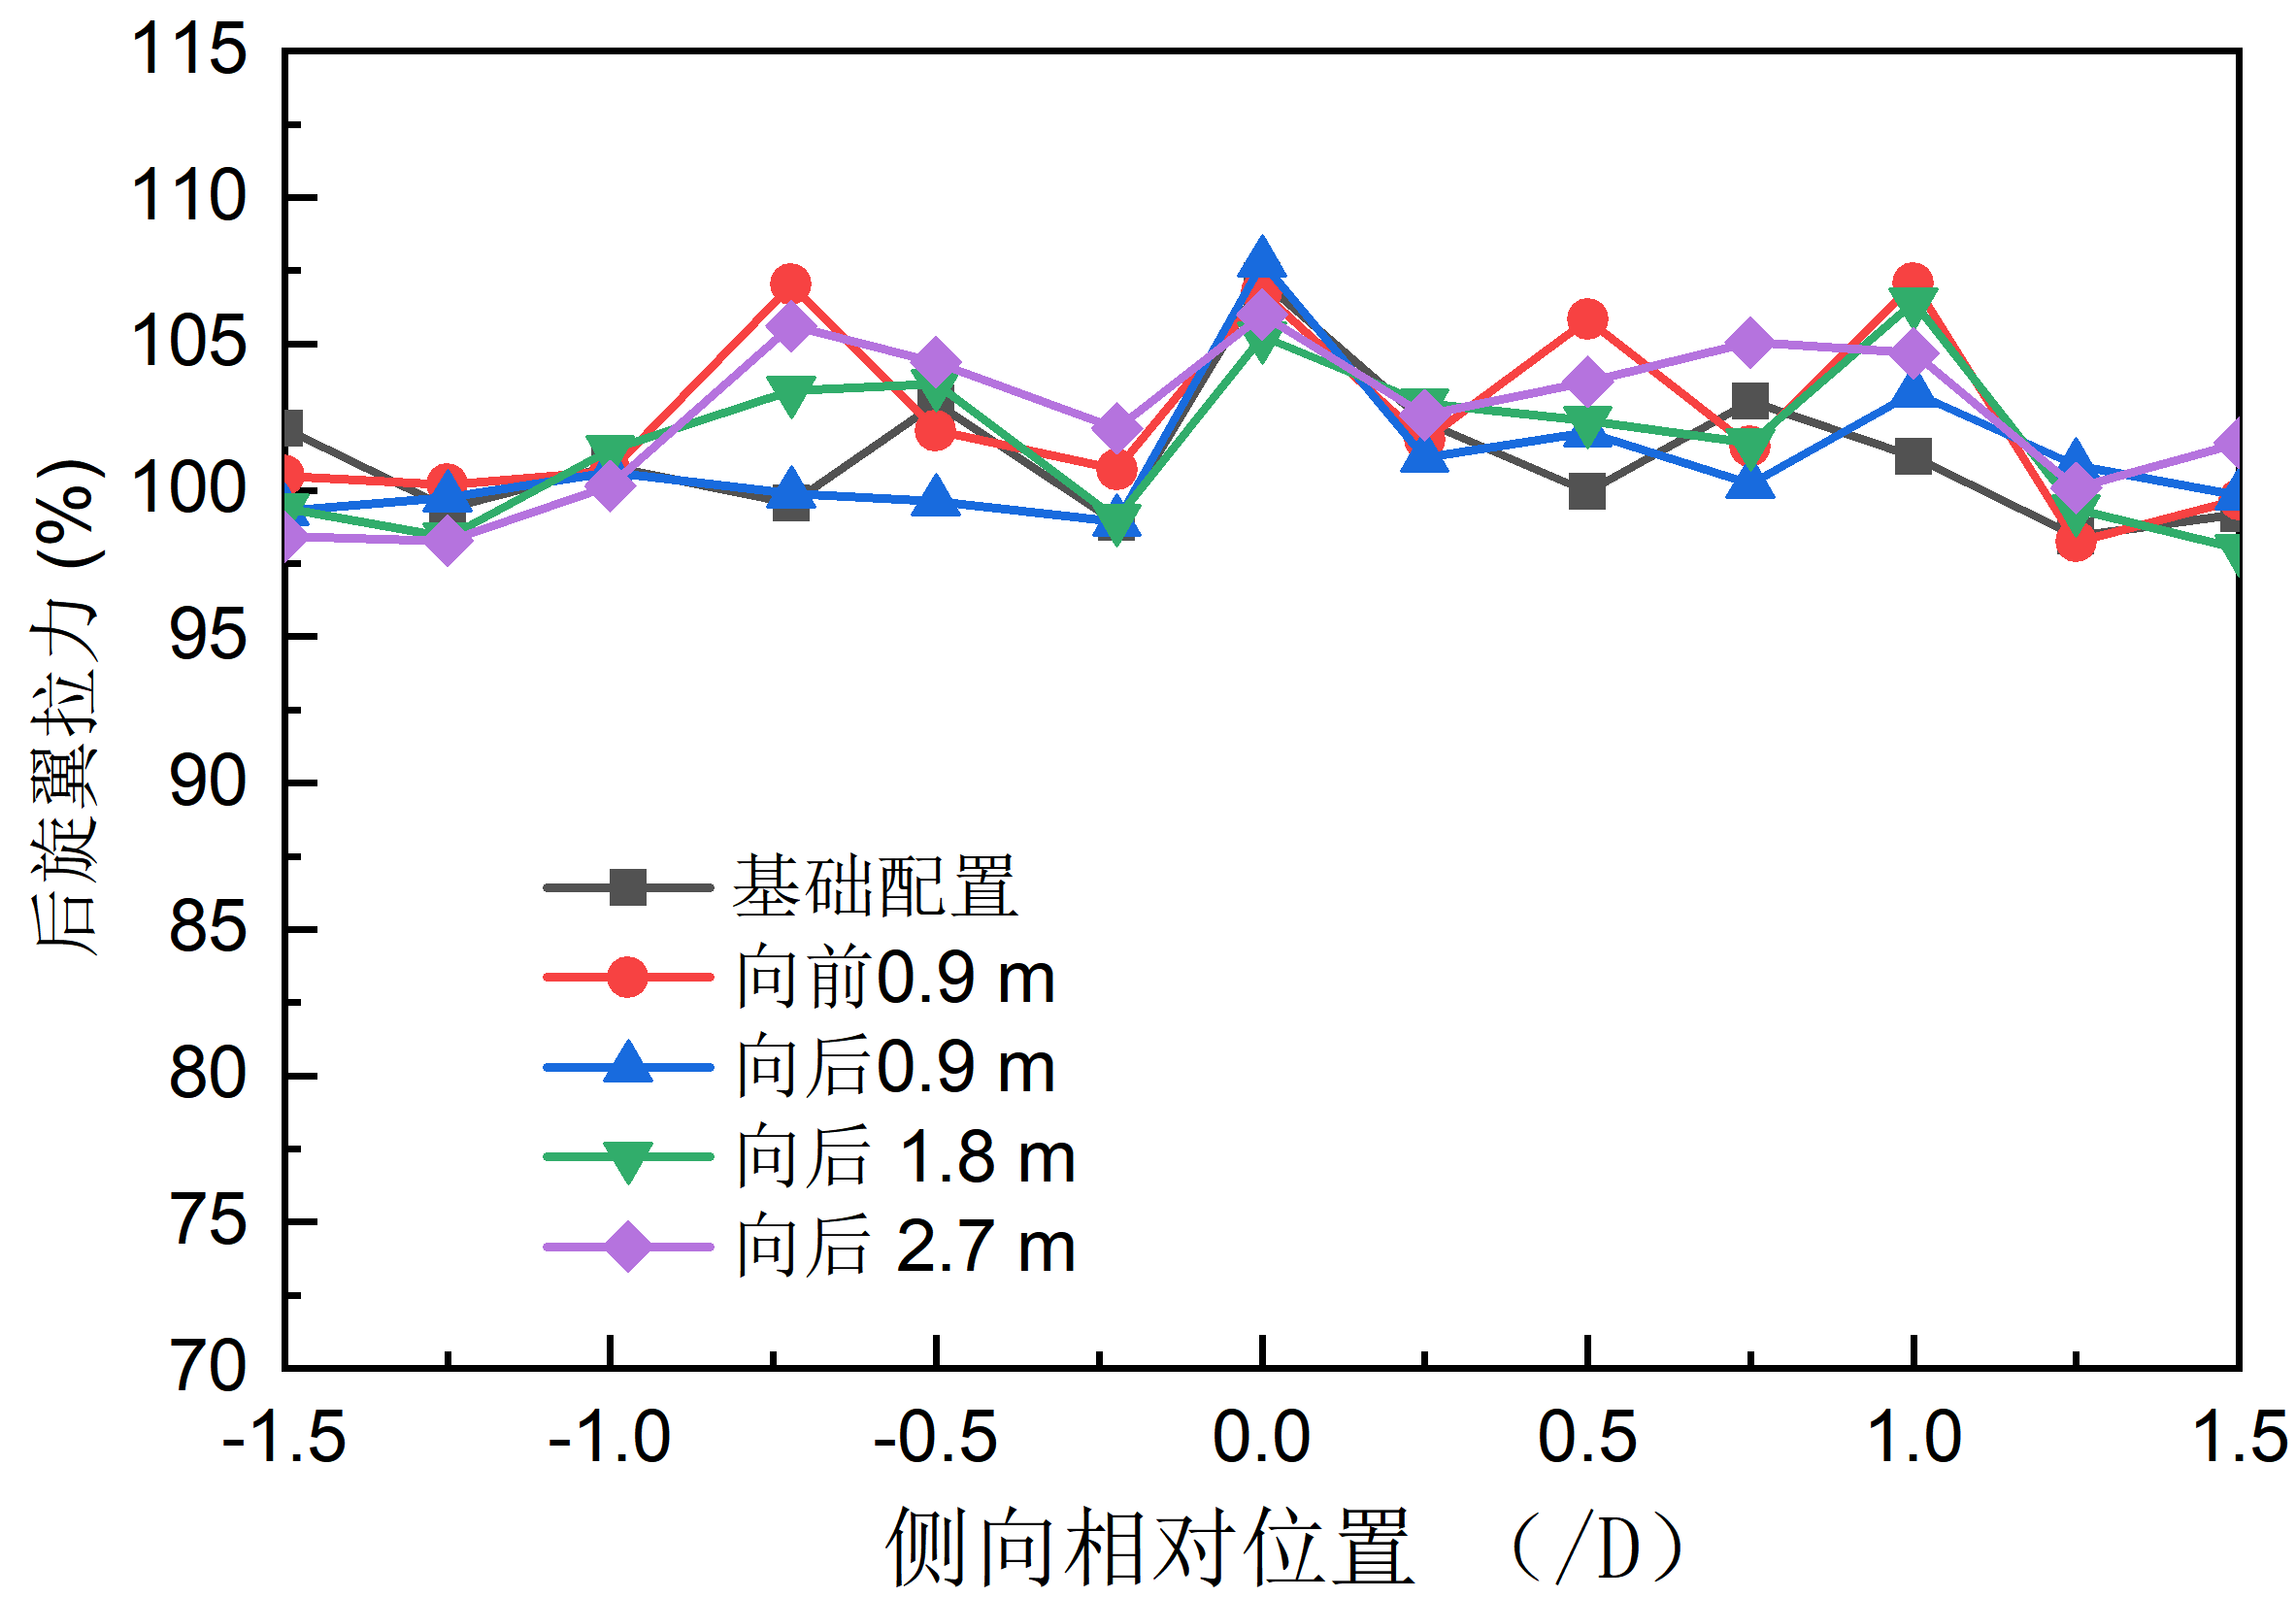
\includegraphics[width=7cm]{fig/figure_chap3/chap_3_5_3_6.png}}
  \caption{不同纵向相对位置下的旋翼拉力}
  \label{fig:chap3_5_3_3}
\end{figure}

\begin{figure}[!htb]
  \centering
  \subfloat[前旋翼]{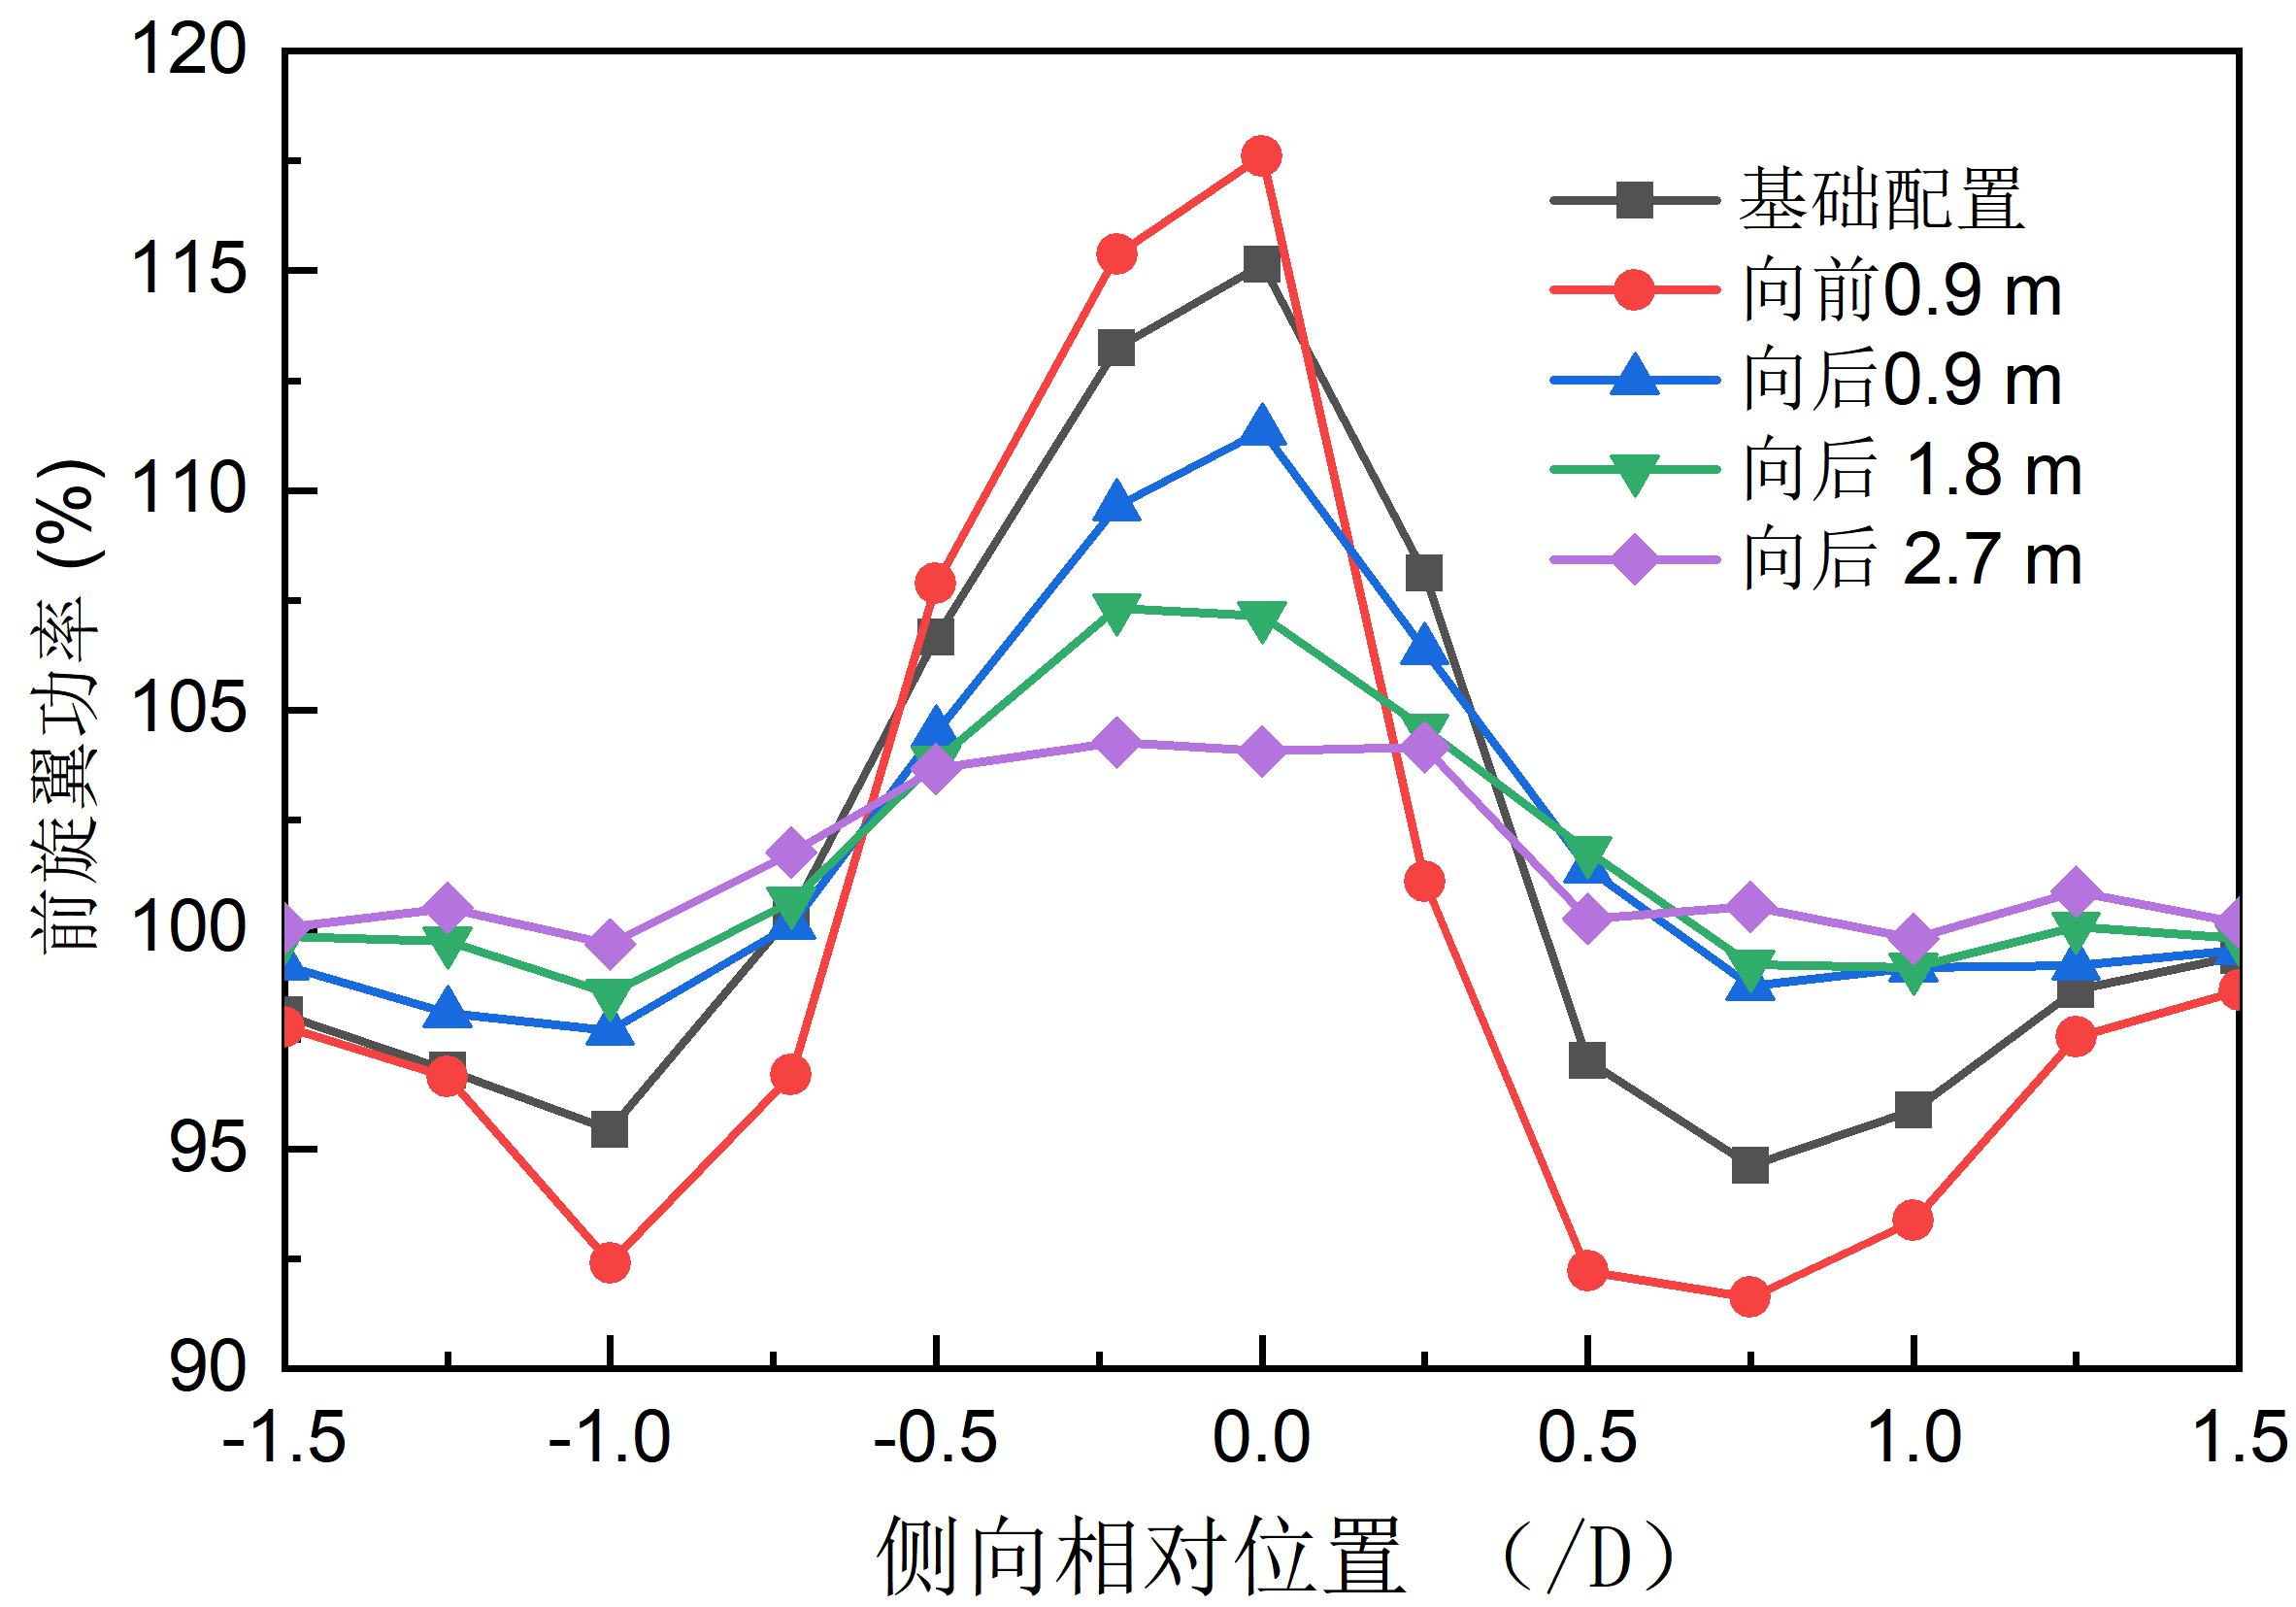
\includegraphics[width=7cm]{fig/figure_chap3/chap_3_5_3_7.png}}\quad
  \subfloat[后旋翼]{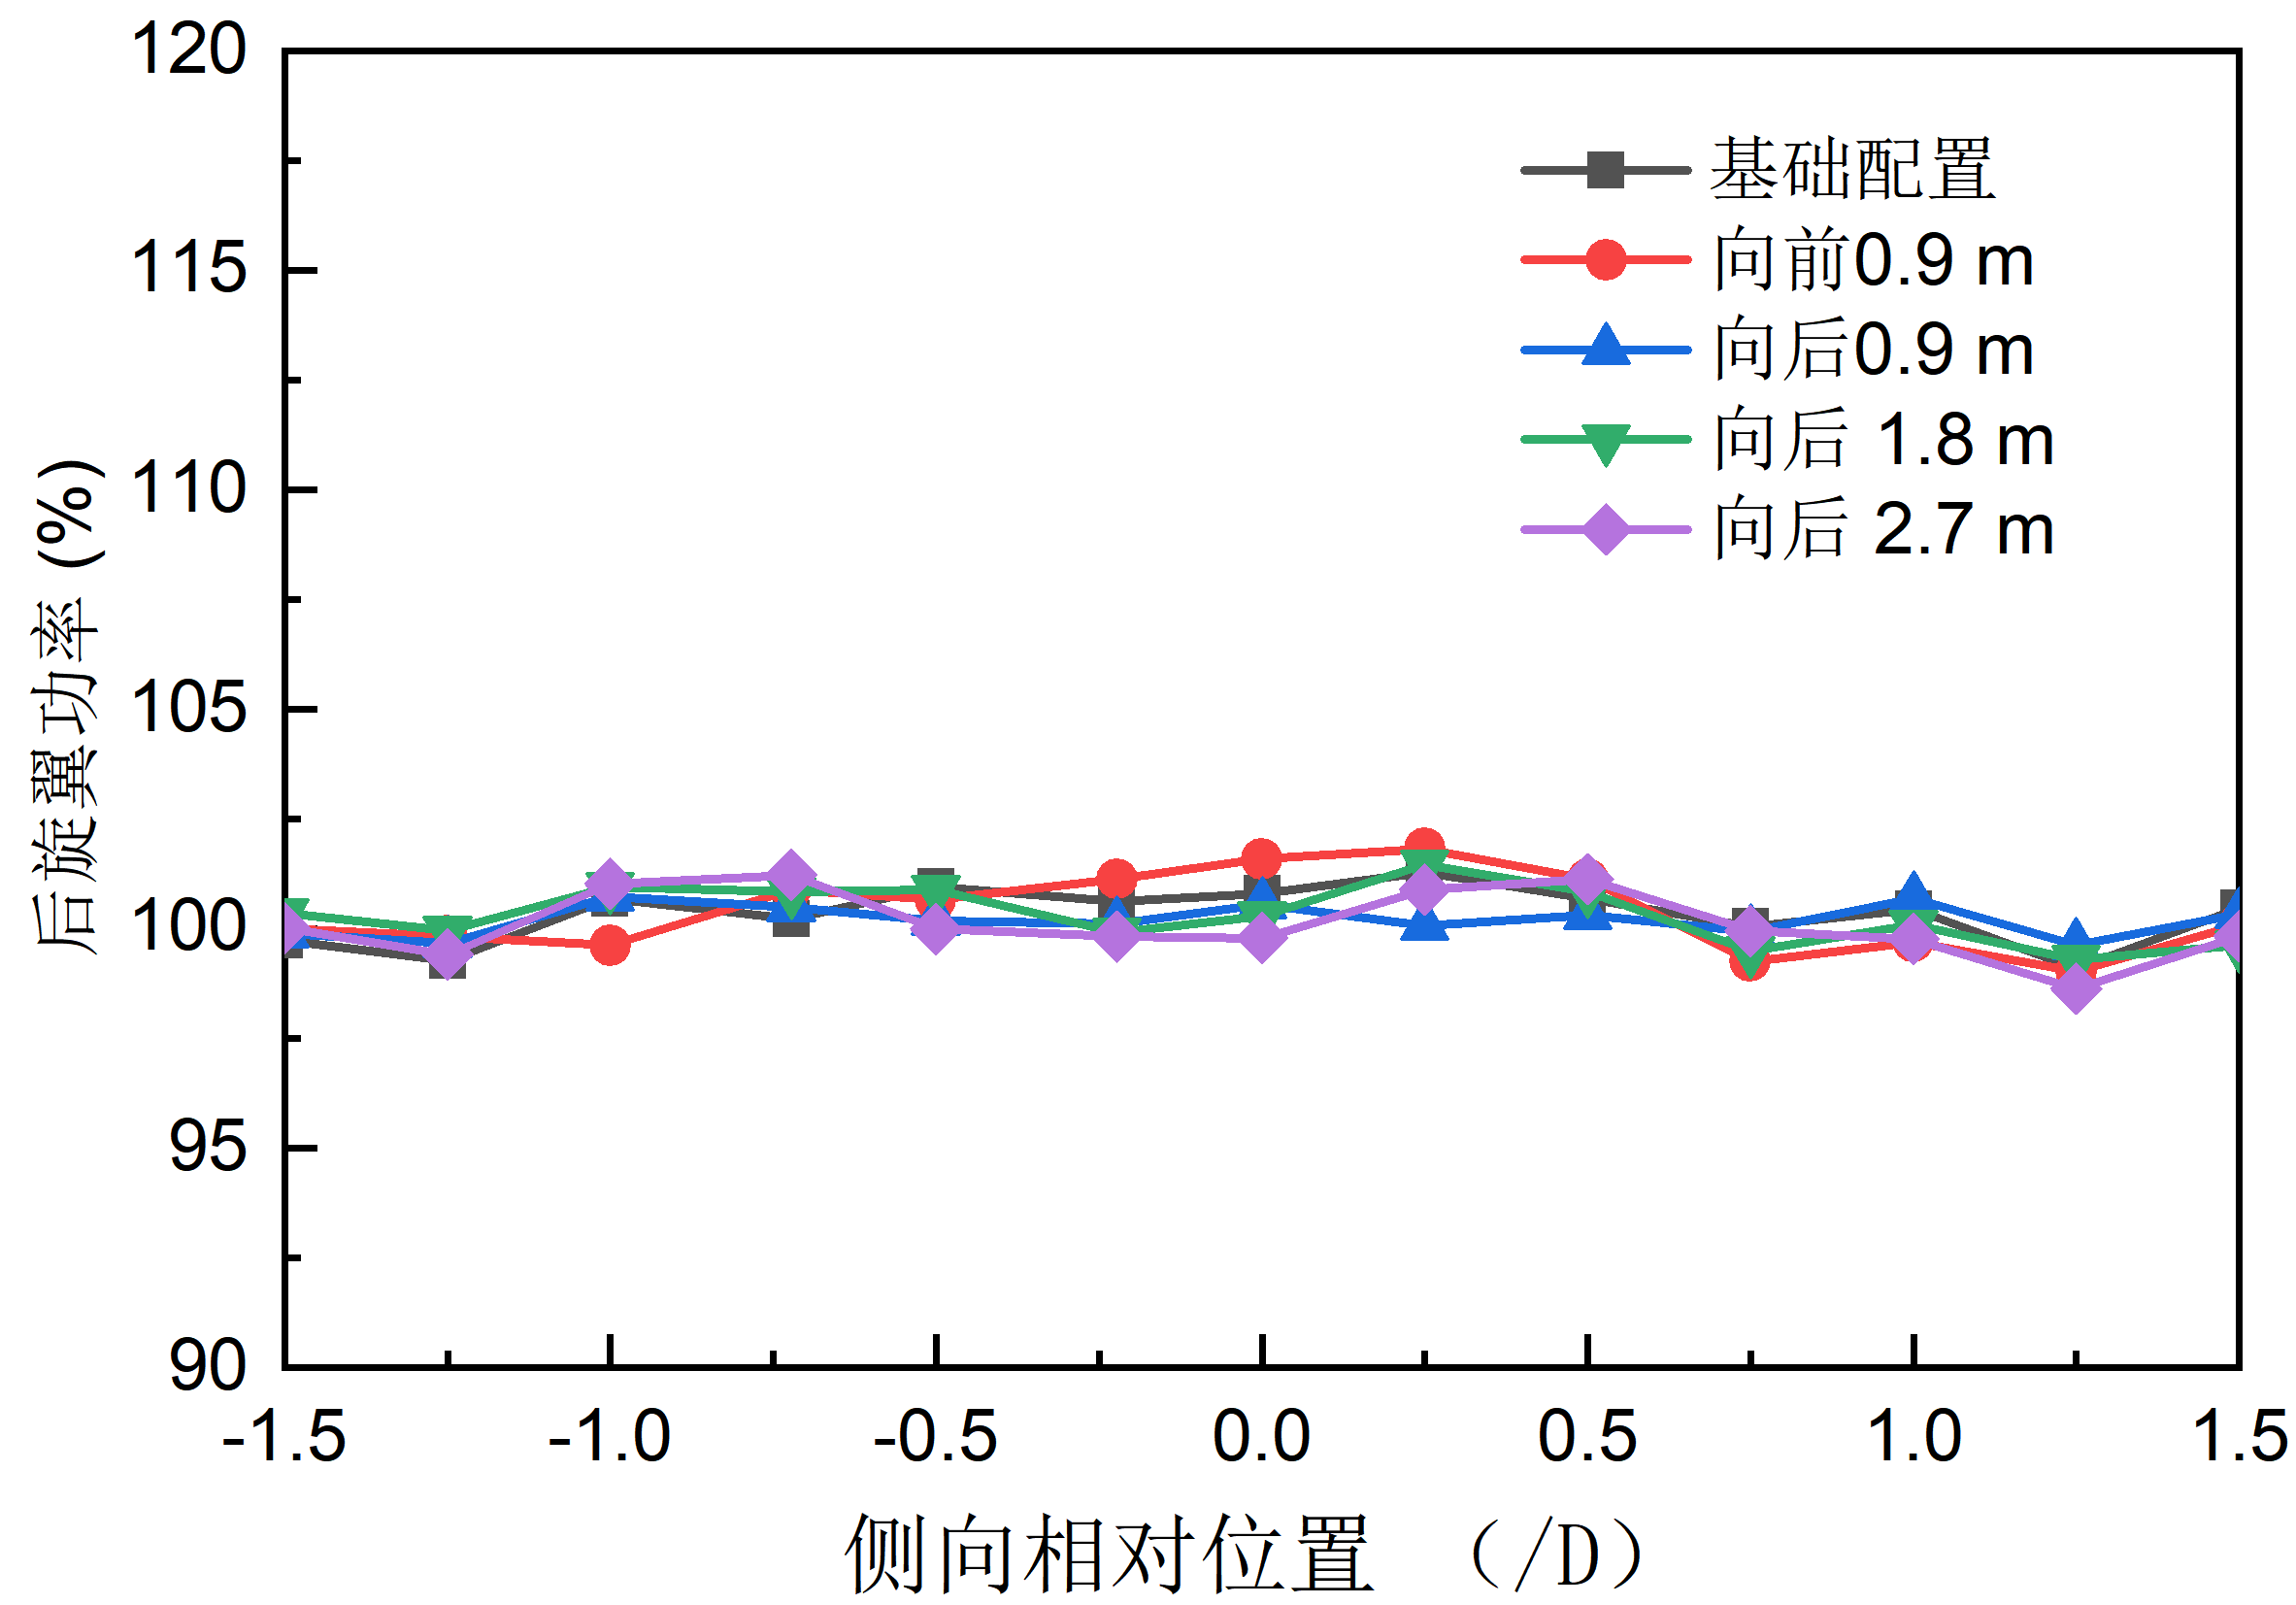
\includegraphics[width=7cm]{fig/figure_chap3/chap_3_5_3_8.png}}
  \caption{不同纵向相对位置下的旋翼功率}
  \label{fig:chap3_5_3_4}
\end{figure}
\subsection{不同垂向相对位置下气动干扰及性能的变化}
图\ref{fig:chap3_5_4_1}给出了直升机协同吊挂系统不同垂向相对位置下的涡度场。可以看出,在基础配置中直升机1的前半部分沉浸在直升机4的尾流中。当直升机1上移0.7 m后,直升机1和直升机4间几乎没有气动干扰。当直升机1下移0.7 m后,直升机1完全沉浸在直升机4的尾流中。
\begin{figure}[!htb]
  \centering
  \subfloat[基本配置]{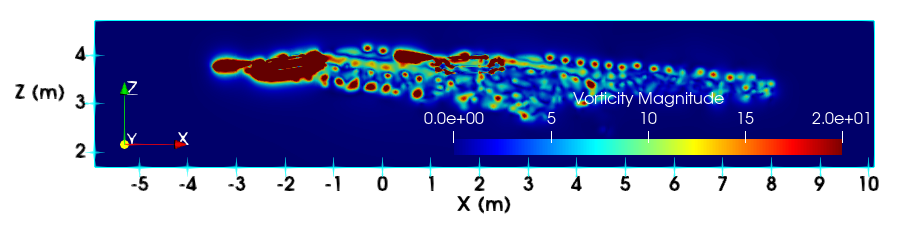
\includegraphics[width=7cm]{fig/figure_chap3/chap_3_5_4_1.png}}\\ 
  \subfloat[上移0.7 m]{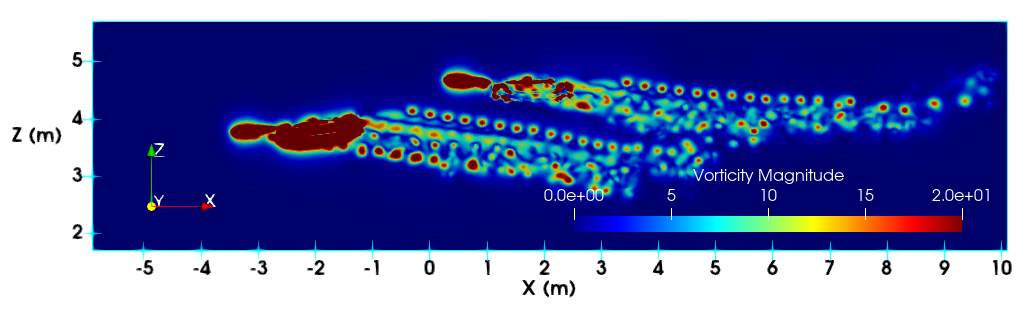
\includegraphics[width=7cm]{fig/figure_chap3/chap_3_5_4_2.png}}\quad
  \subfloat[下移0.7 m]{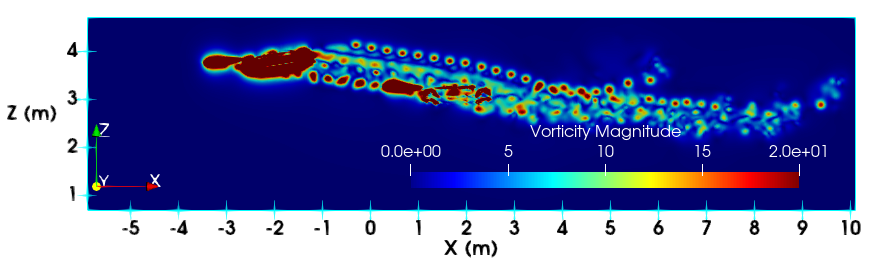
\includegraphics[width=7cm]{fig/figure_chap3/chap_3_5_4_3.png}}
  \caption{直升机协同吊挂系统不同垂向相对位置下的涡度场}
  \label{fig:chap3_5_4_1}
\end{figure}

图\ref{fig:chap3_5_4_2}给出了不同垂向相对位置下0.75 R处的截面力。当直升机1上移0.7 m时,从方位角100 \degree 到250 \degree,前旋翼的截面拉力相比其他两种情况更大、
波动更小。当直升机1下移0.7 m时,后旋翼的截面拉力比其他两种情况小。这是因为直升机1下移0.7 m时,直升机1完全沉浸在直升机4的尾流中。
\begin{figure}[!htb]
  \centering
  \subfloat[前旋翼]{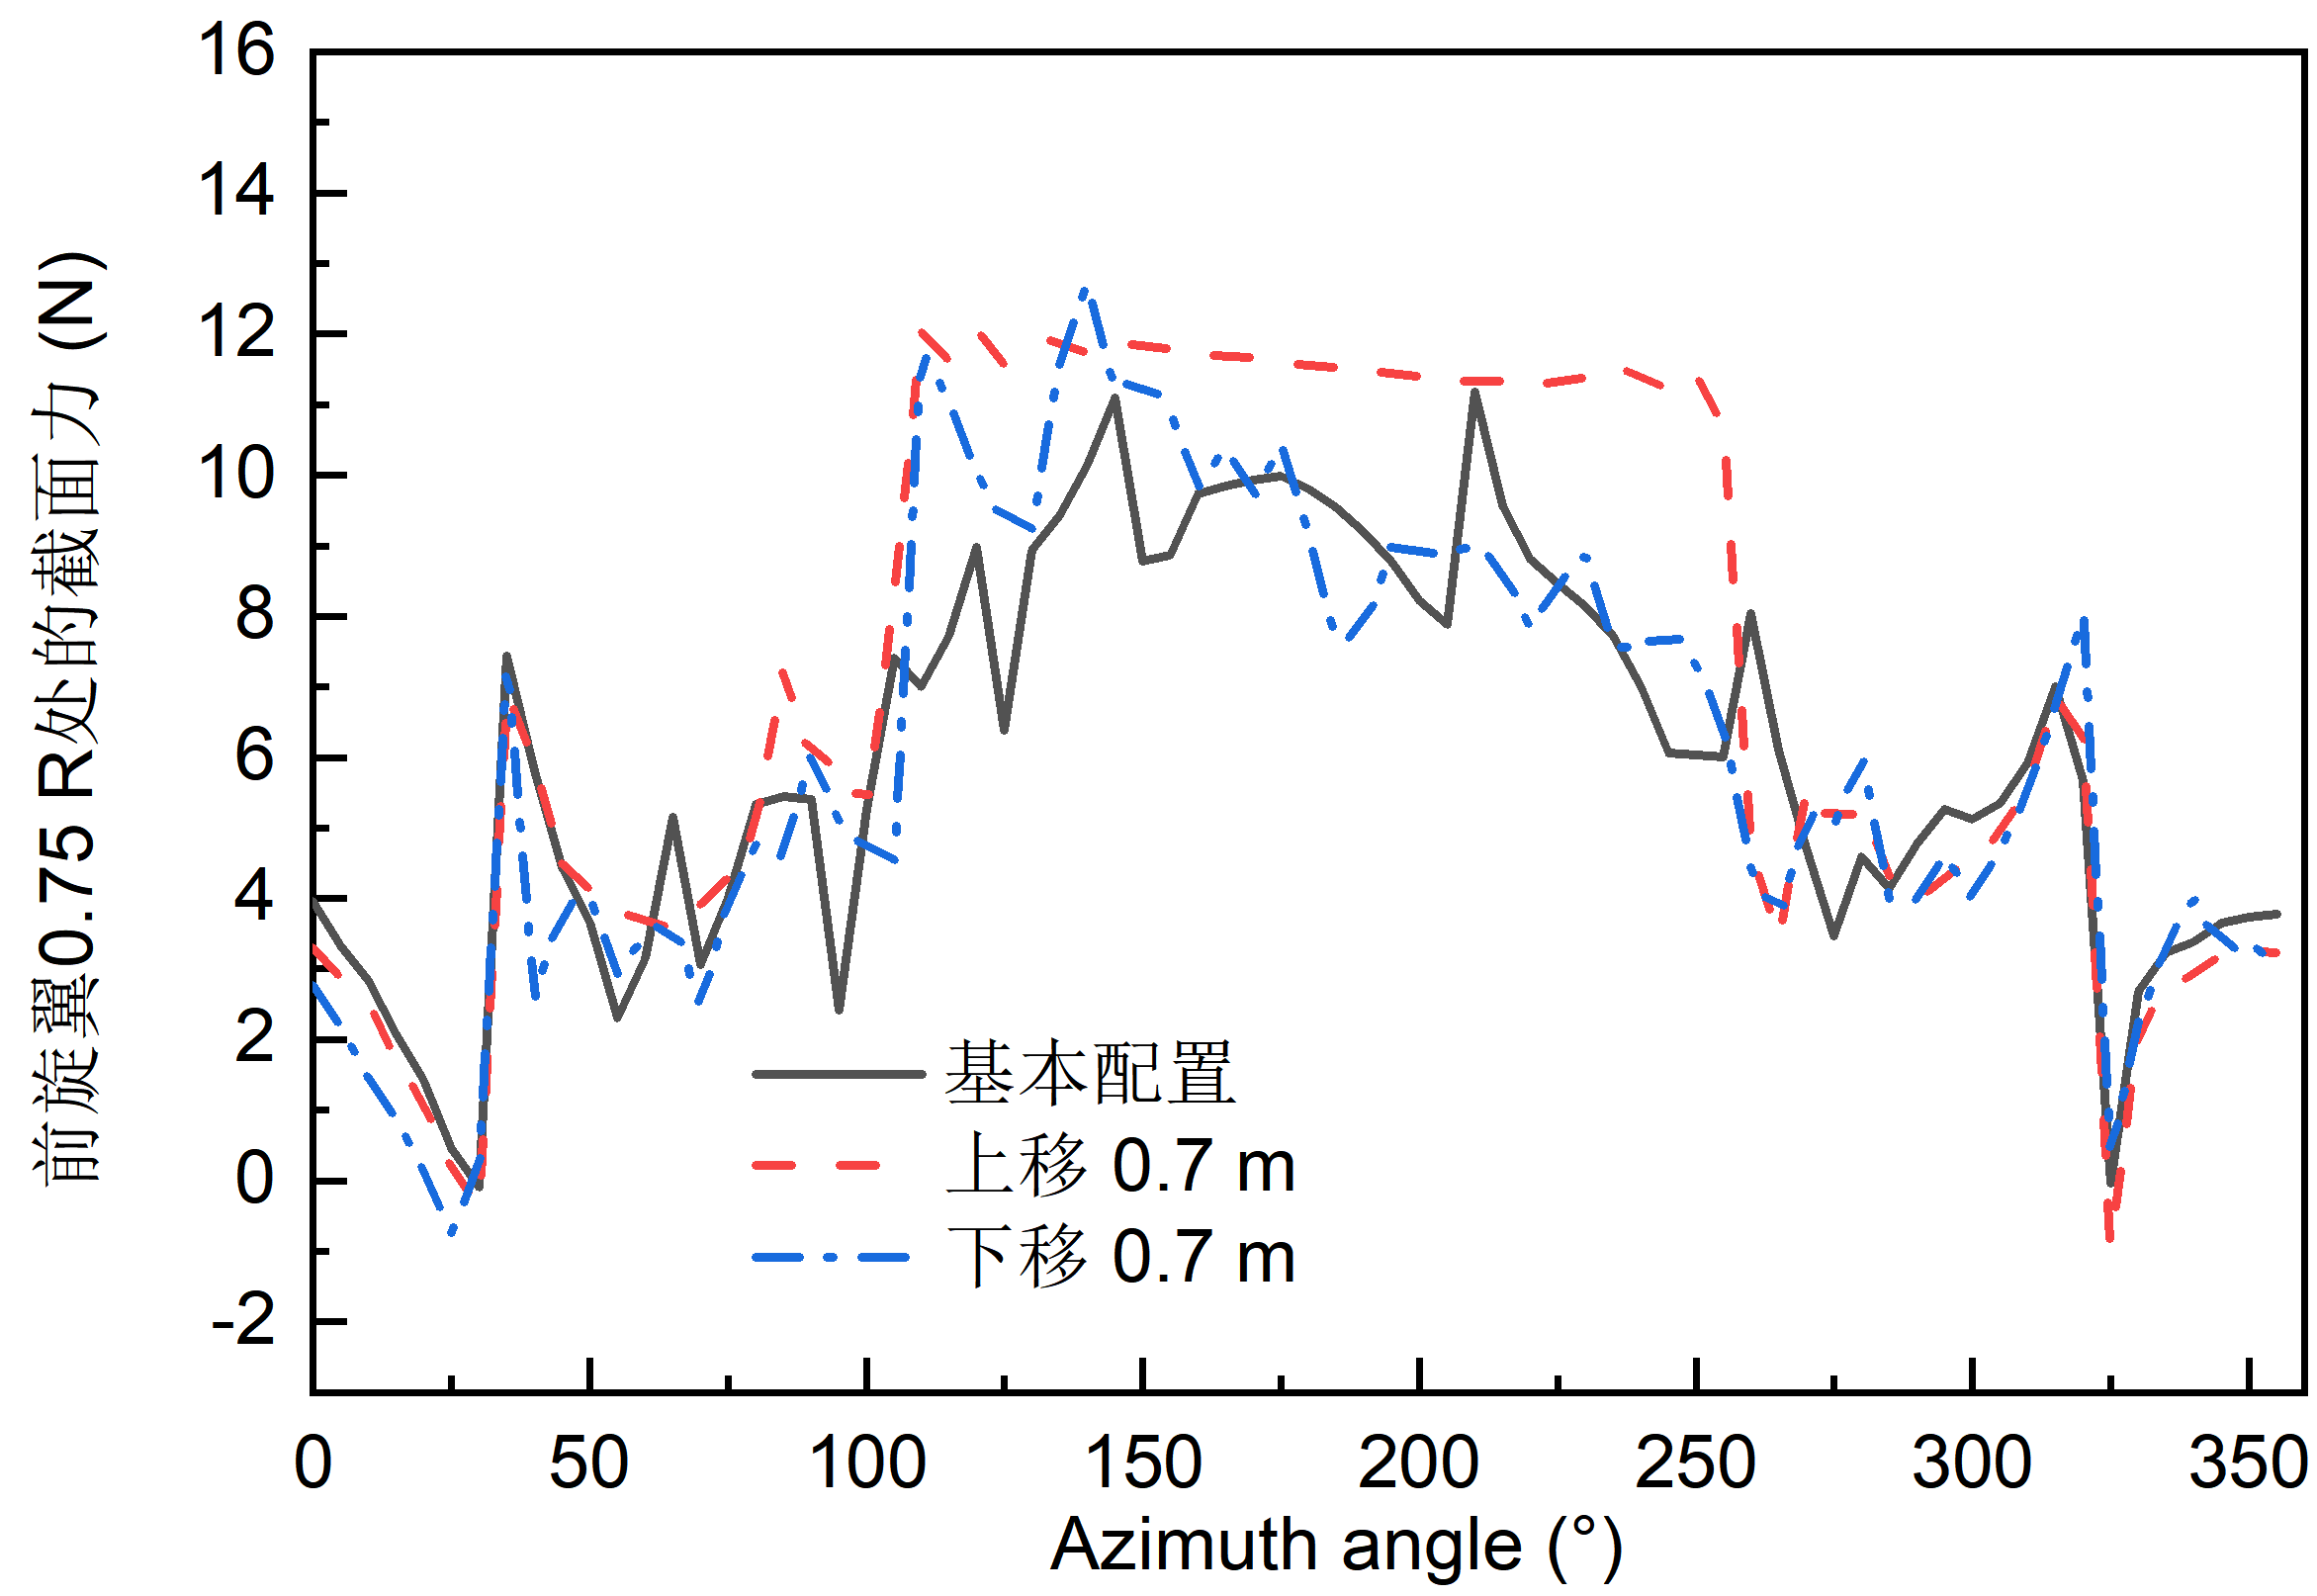
\includegraphics[width=7cm]{fig/figure_chap3/chap_3_5_4_4.png}}\quad
  \subfloat[后旋翼]{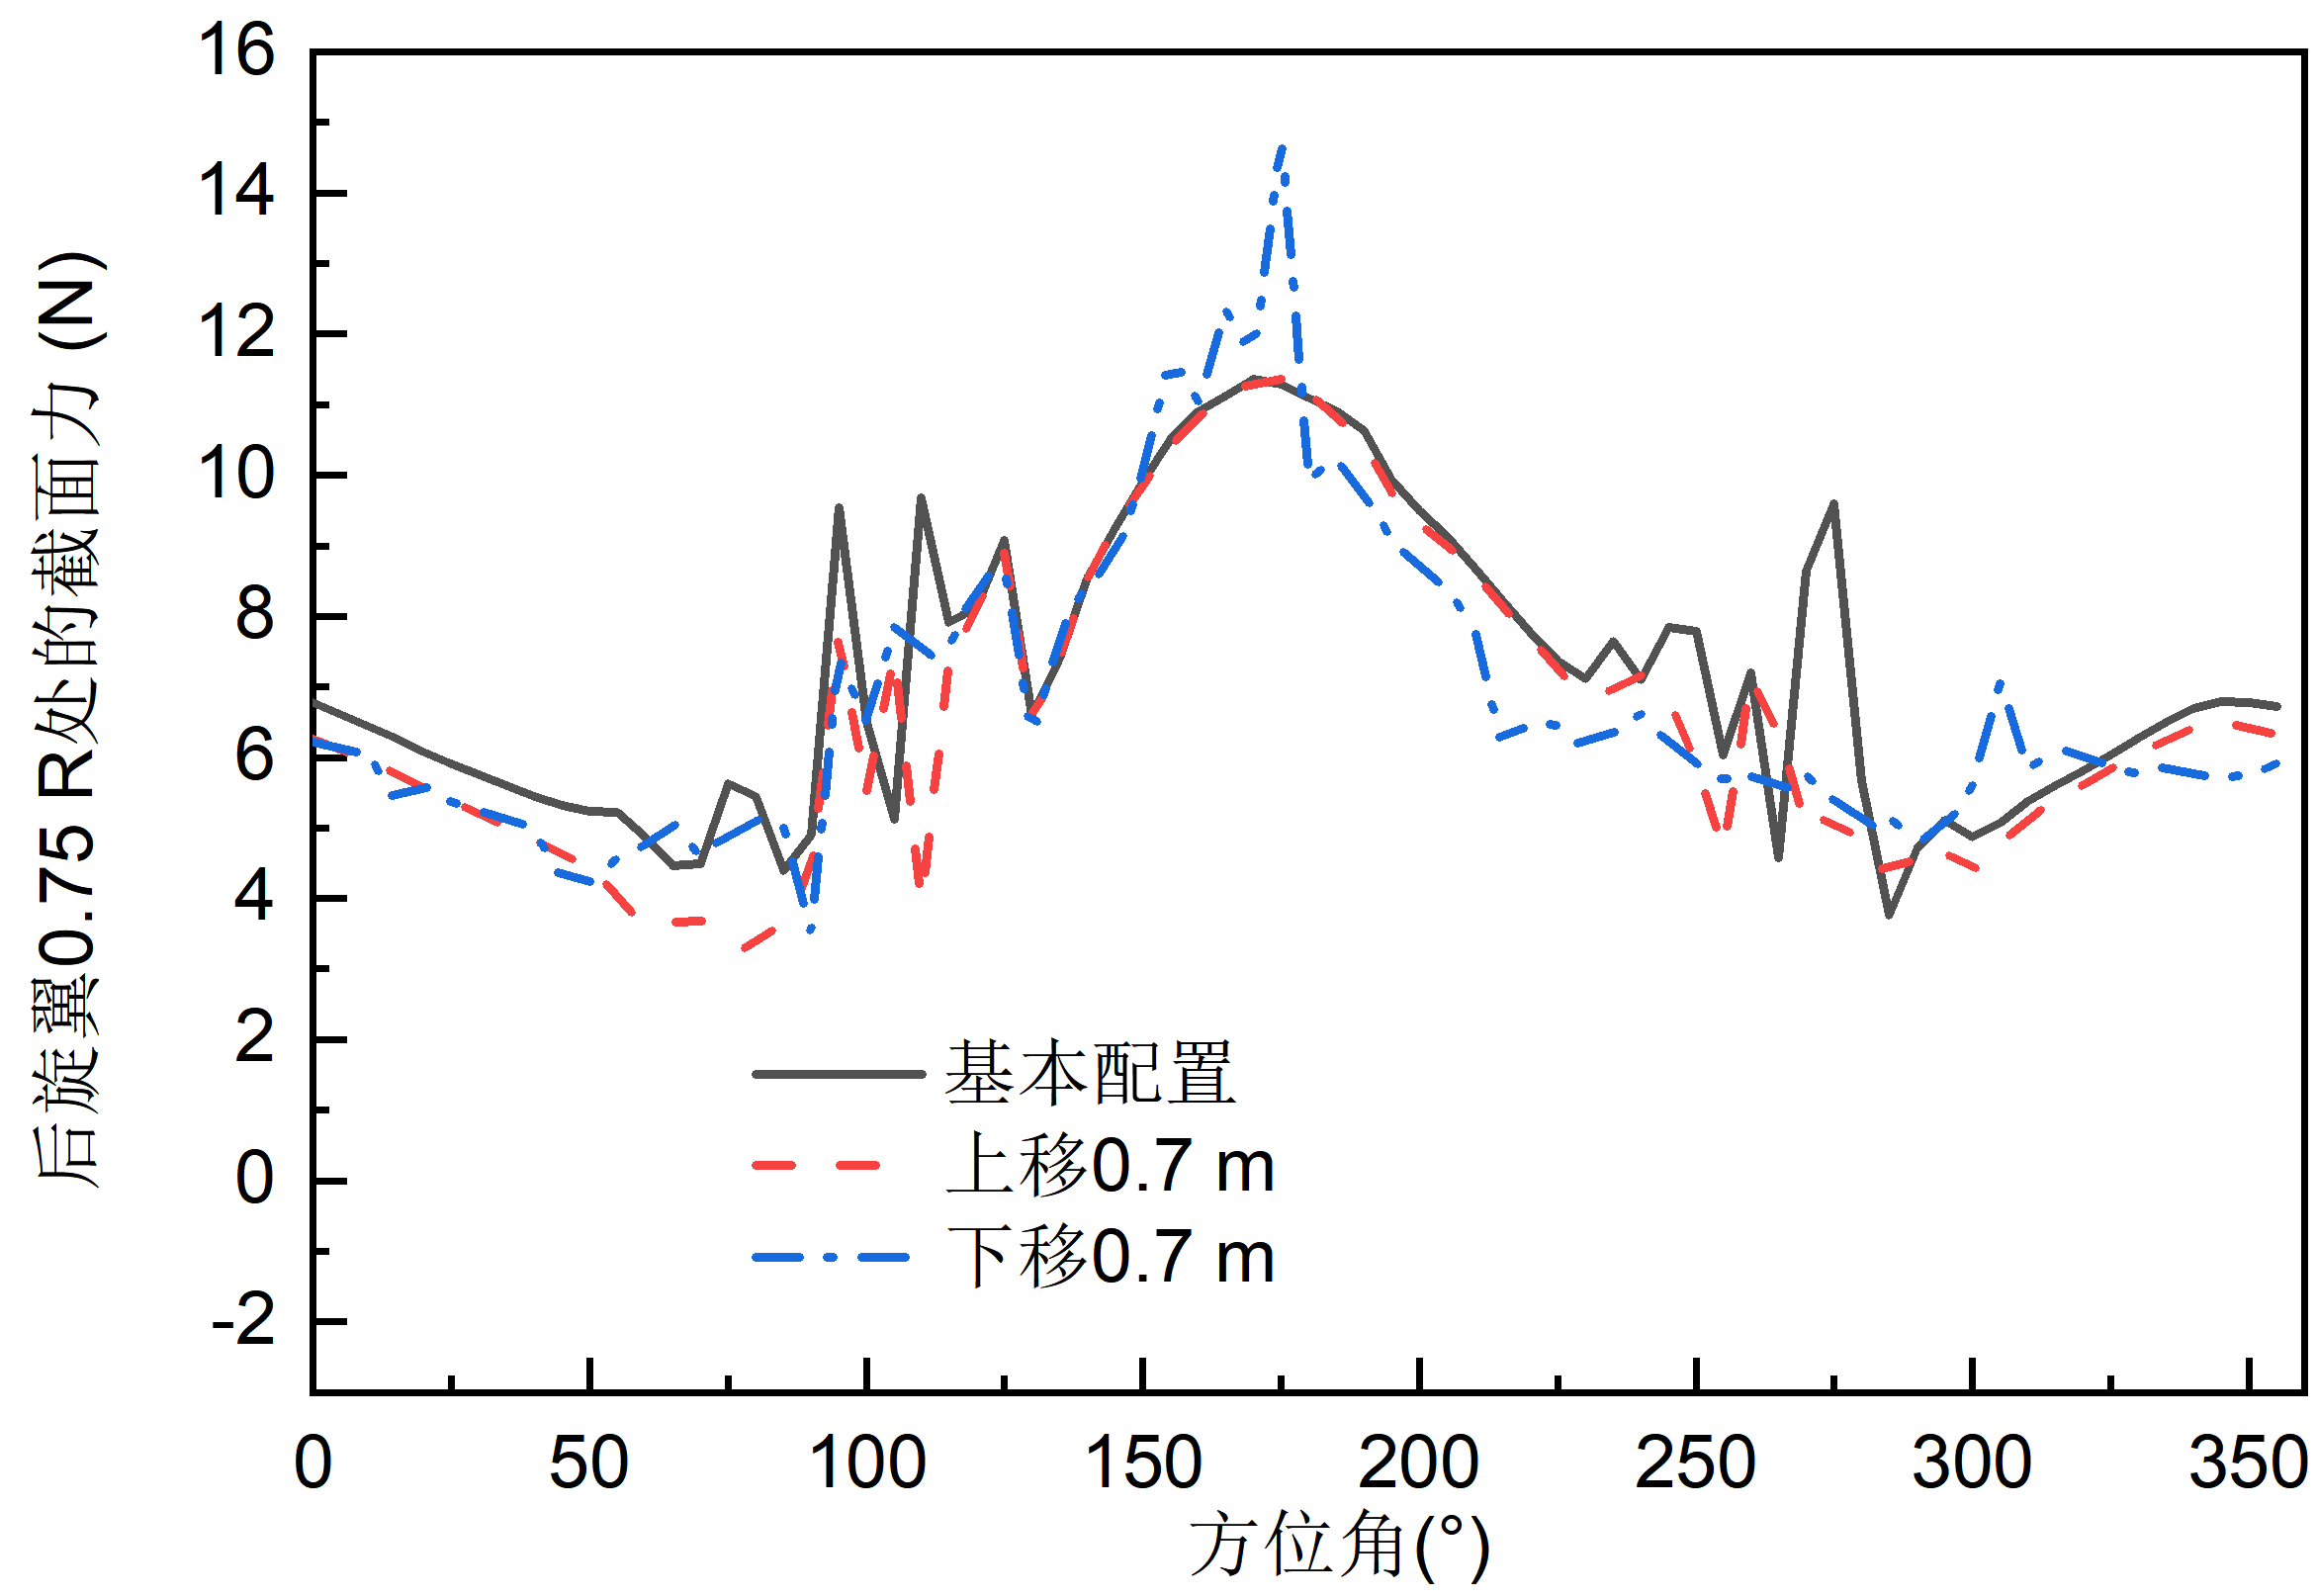
\includegraphics[width=7cm]{fig/figure_chap3/chap_3_5_4_5.png}}
  \caption{不同垂向相对位置下0.75 R 处的截面力}
  \label{fig:chap3_5_4_2}
\end{figure}

图\ref{fig:chap3_5_4_3}(a)和图\ref{fig:chap3_5_4_4}(a)给出了不同垂向相对位置下直升机1前旋翼拉力和功率的变化。对于基础配置和直升机1下移0.7 m的情况,当垂向相对位置为0时,大约有20\%的拉力损失和15\%的功率增加。当直升机1和直升机4间的侧向相对位置正向或负向增加时,拉力增加,功率减小。对于直升机1上移0.7 m、上移1.4 m、下移1.4 m的情况,拉力、功率与无干扰时相差不大。

图\ref{fig:chap3_5_4_3}(b)和图\ref{fig:chap3_5_4_4}(b)给出了不同垂向相对位置下直升机1后旋翼拉力和功率的变化。可以看出,垂向相对位置变化对后旋翼拉力和功率的影响较小。

\begin{figure}[!htb]
  \centering
  \subfloat[前旋翼]{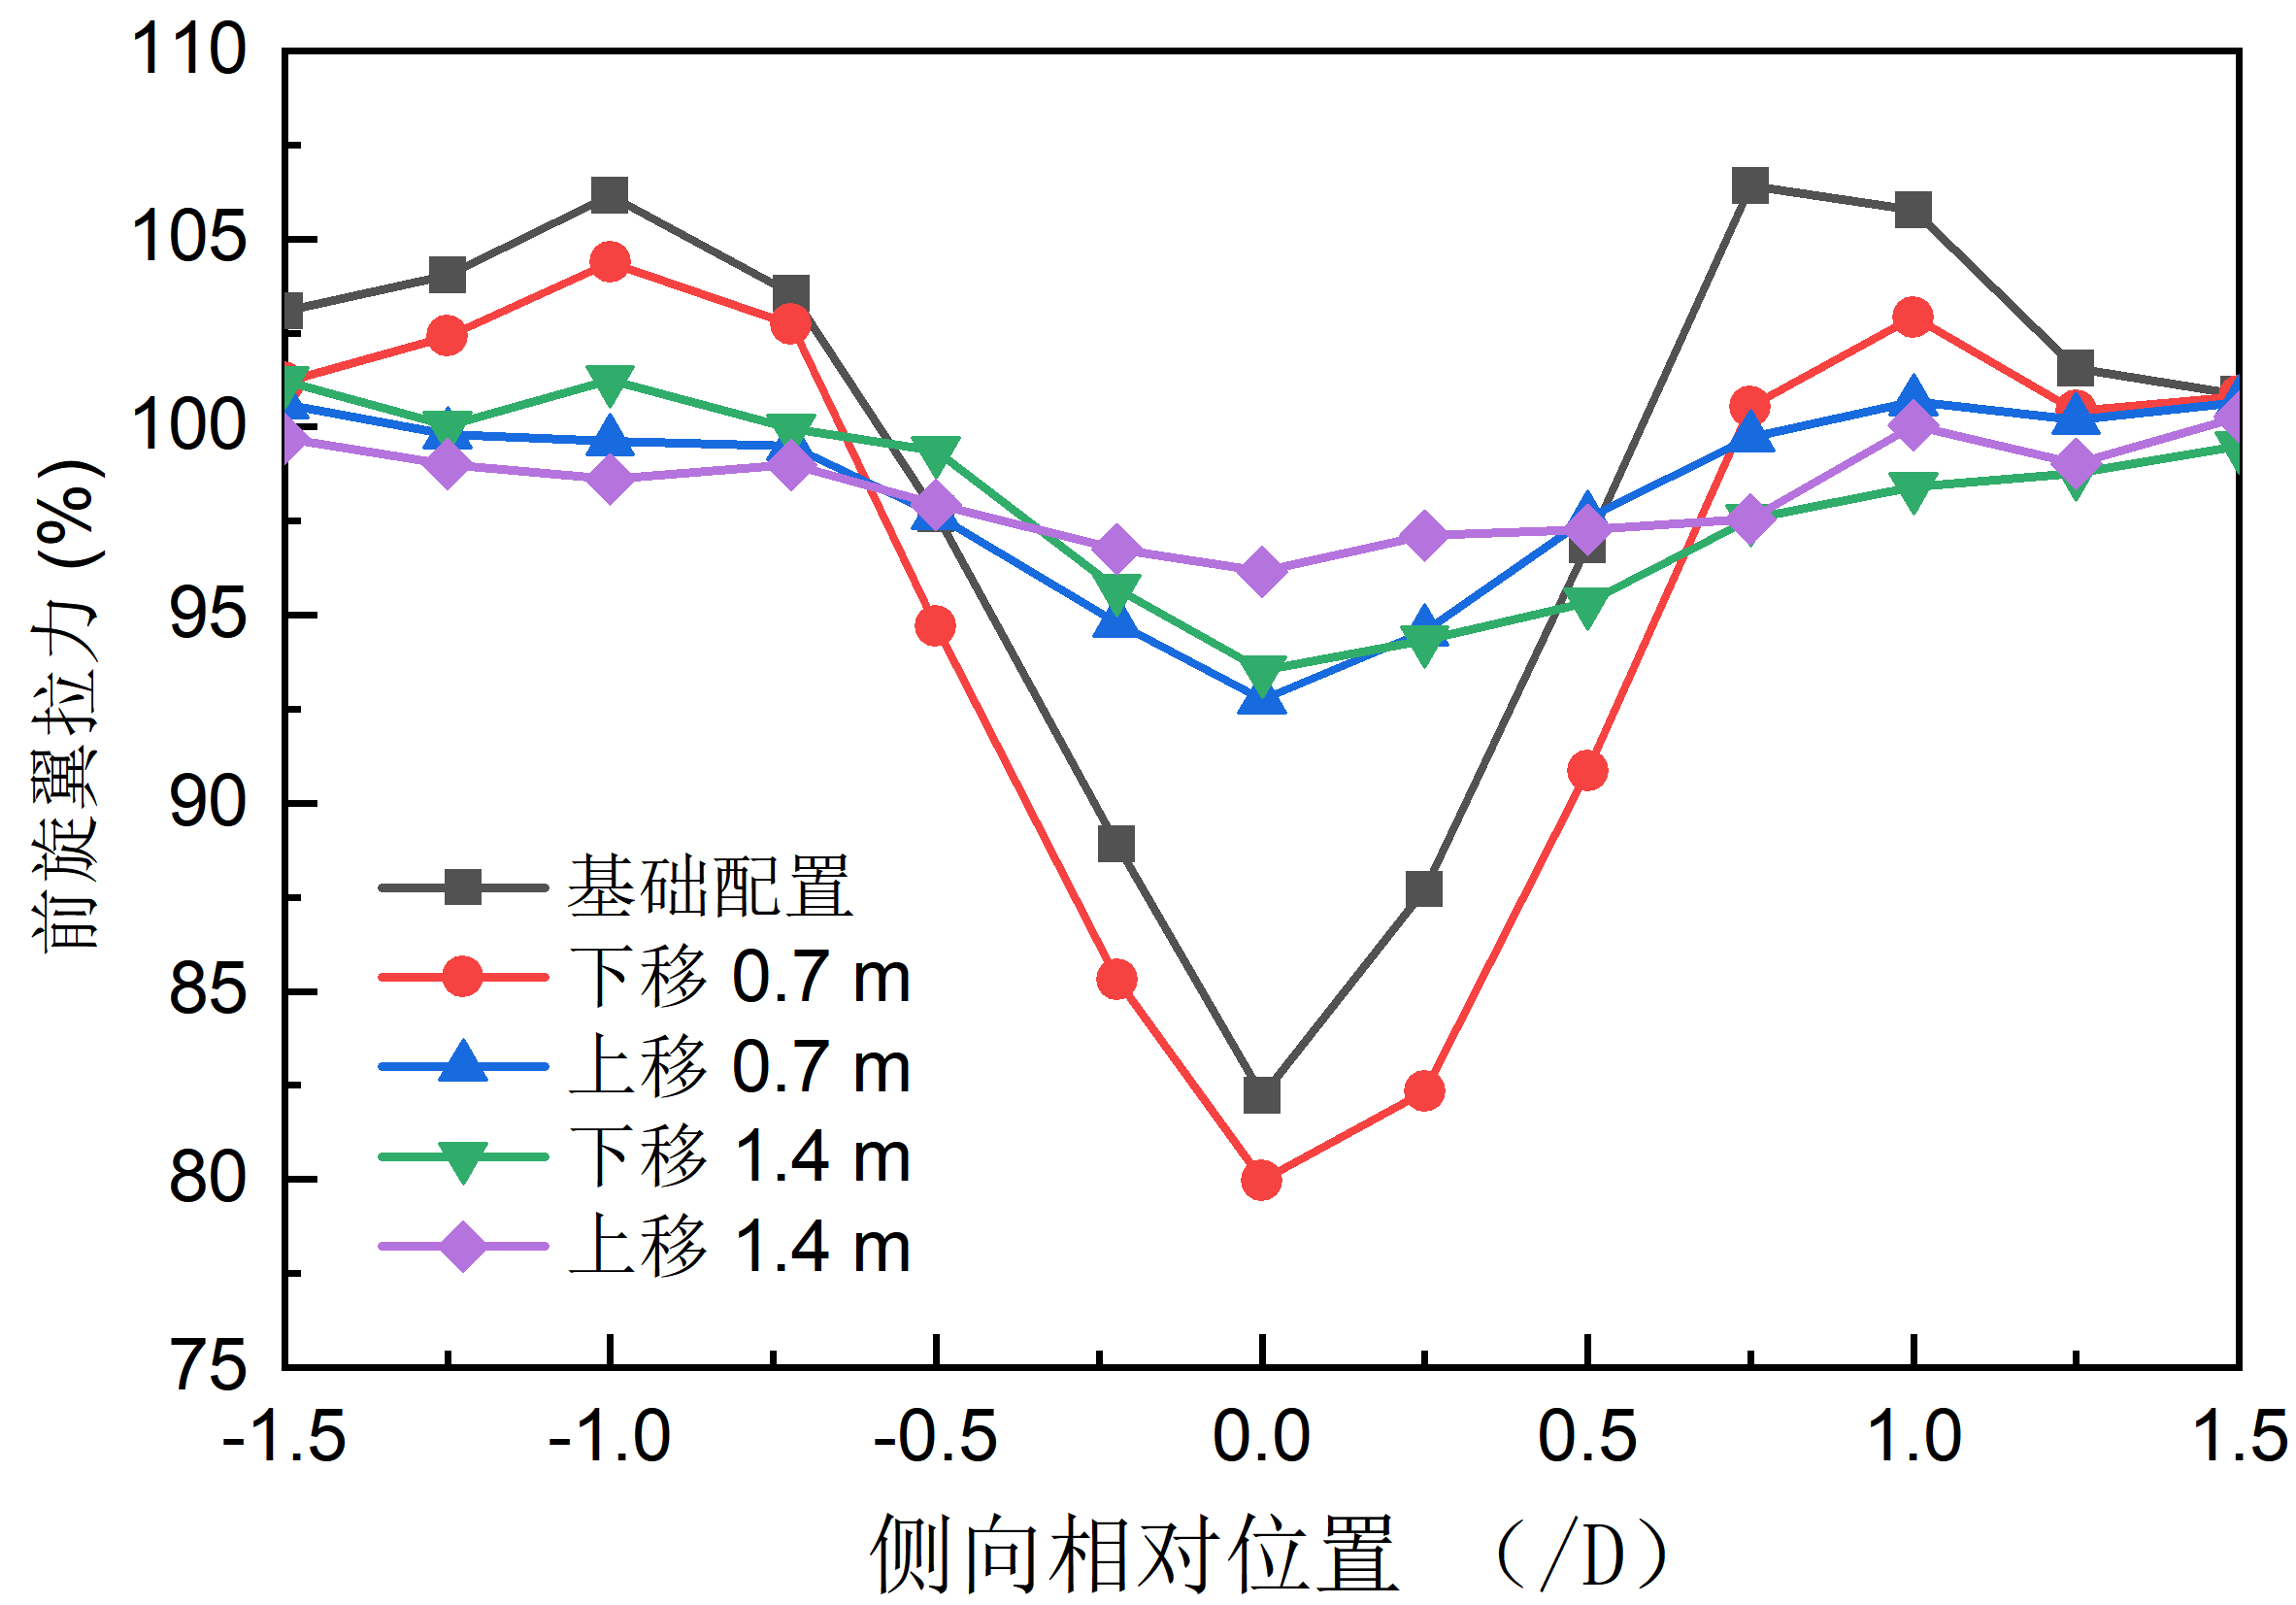
\includegraphics[width=7cm]{fig/figure_chap3/chap_3_5_4_6.png}}\quad
  \subfloat[后旋翼]{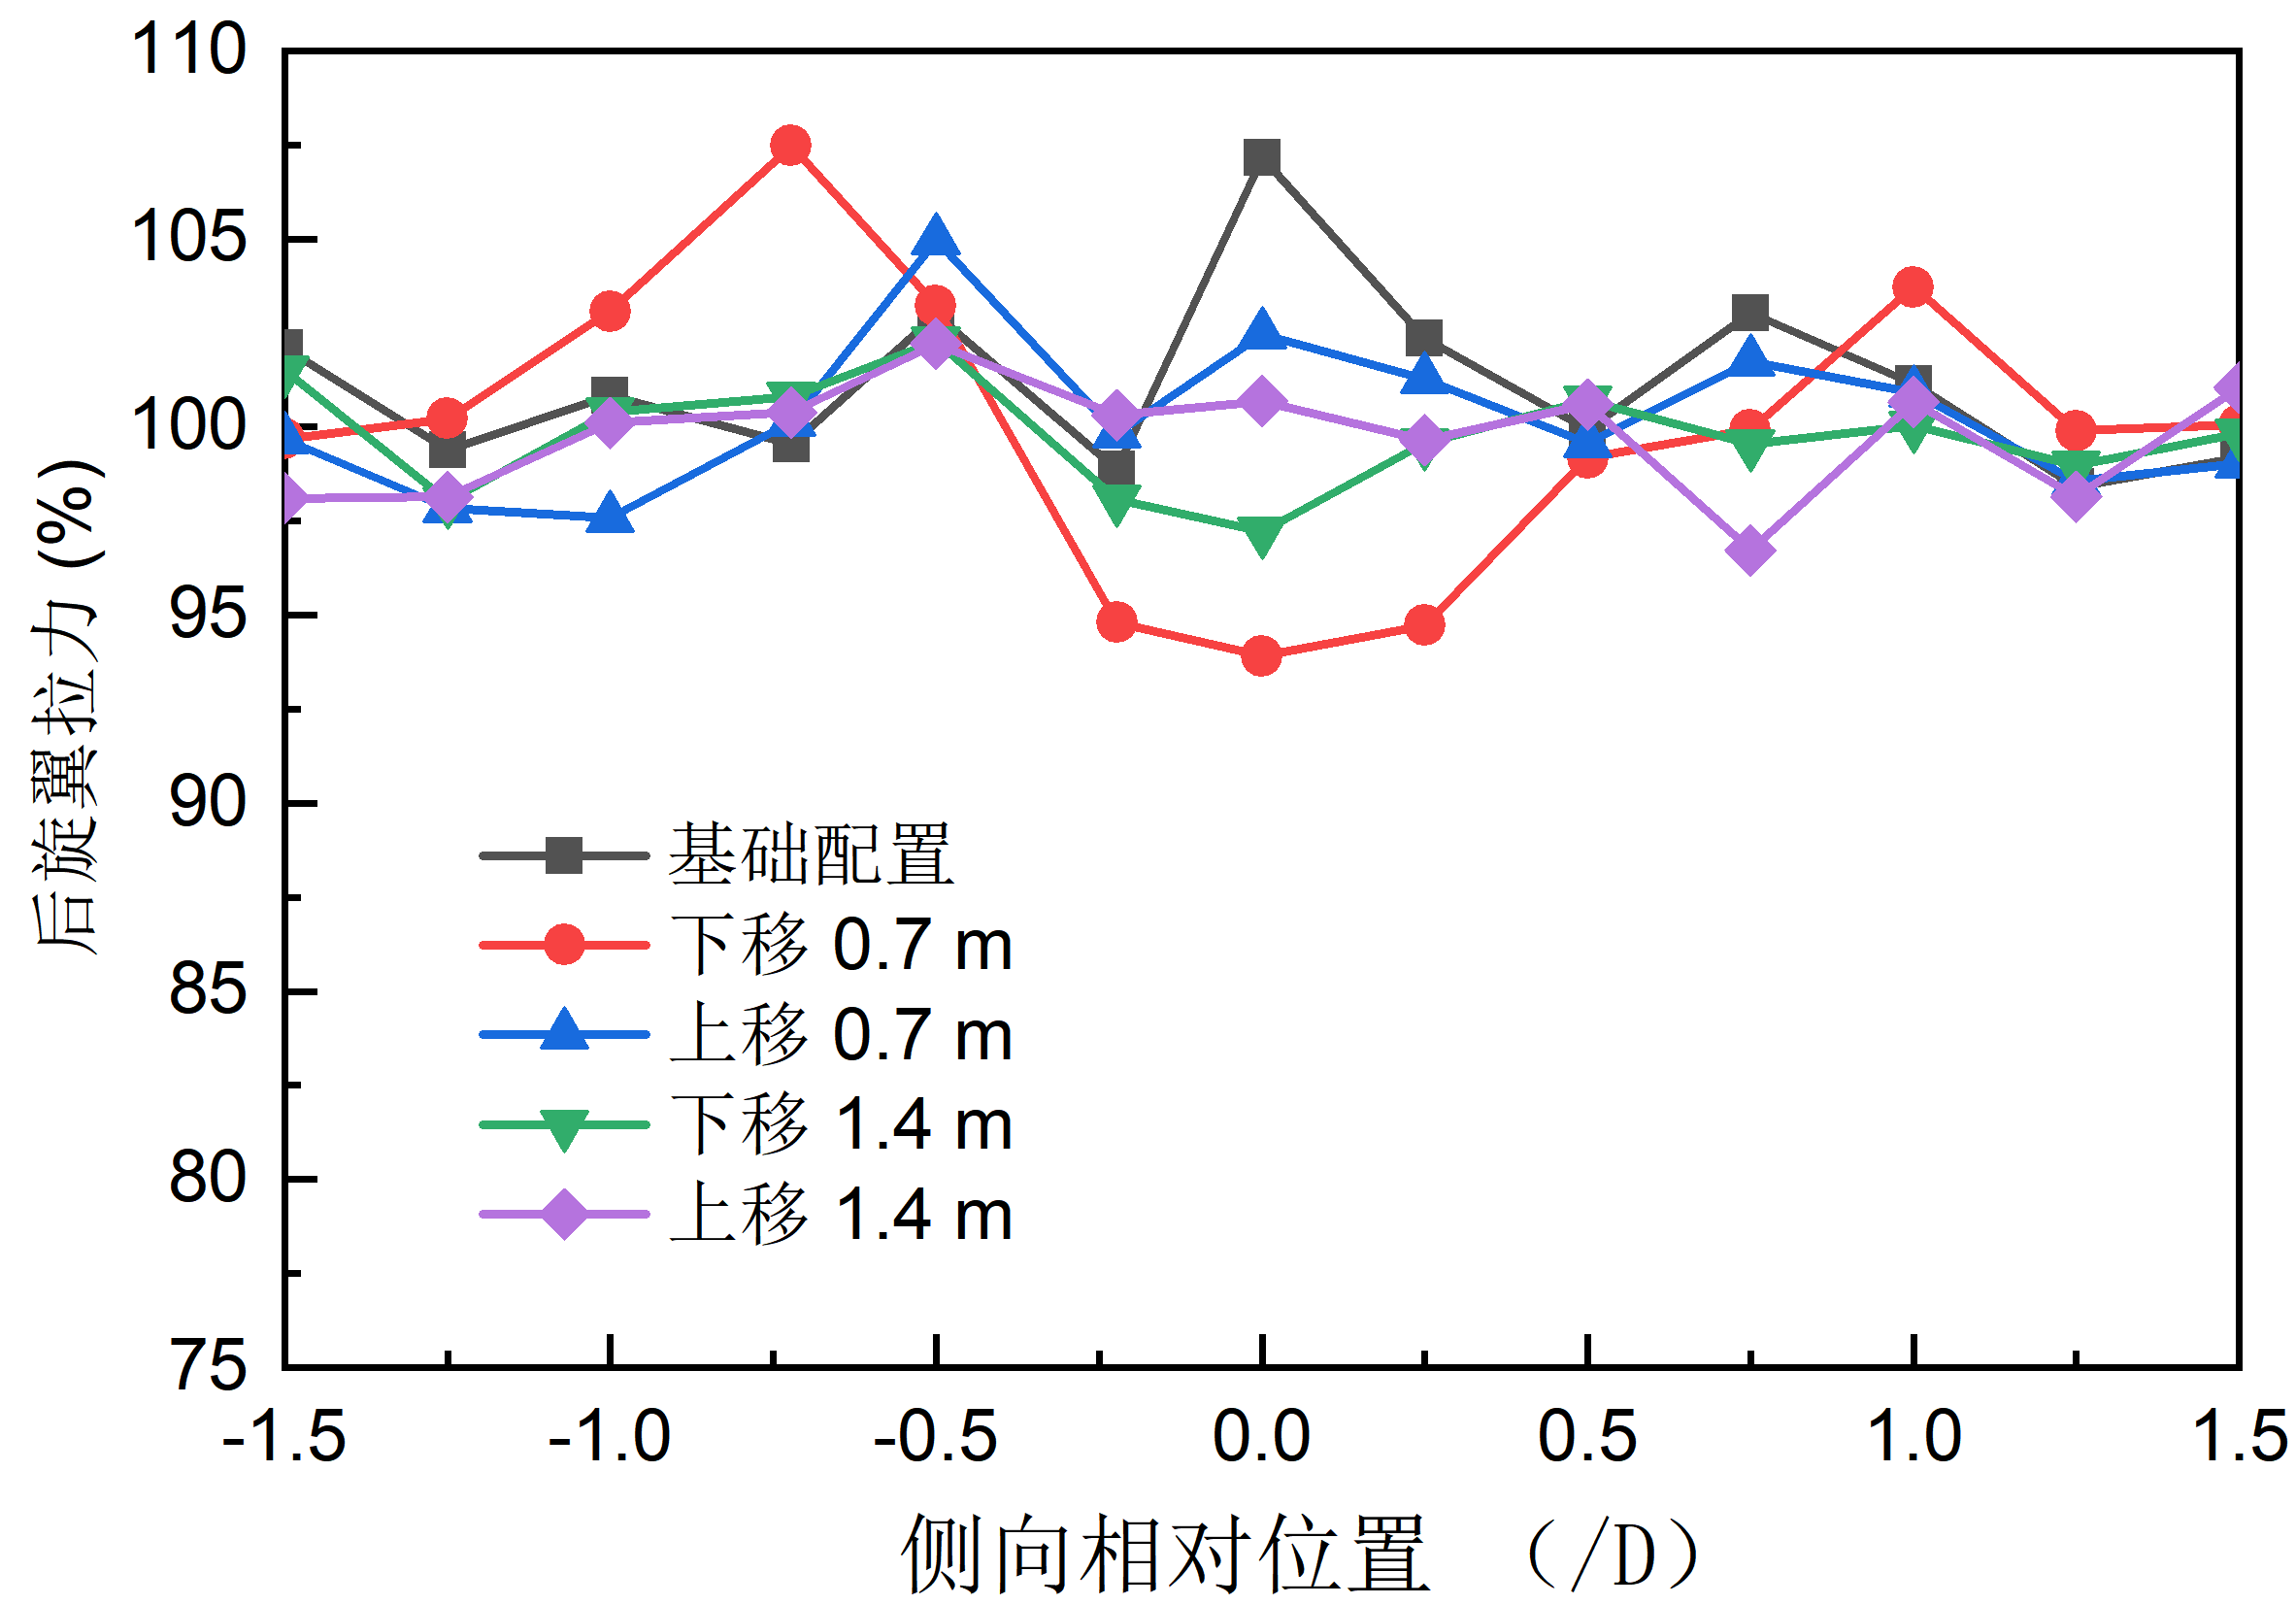
\includegraphics[width=7cm]{fig/figure_chap3/chap_3_5_4_7.png}}
  \caption{不同垂向相对位置下的旋翼拉力}
  \label{fig:chap3_5_4_3}
\end{figure}

\begin{figure}[!htb]
  \centering
  \subfloat[前旋翼]{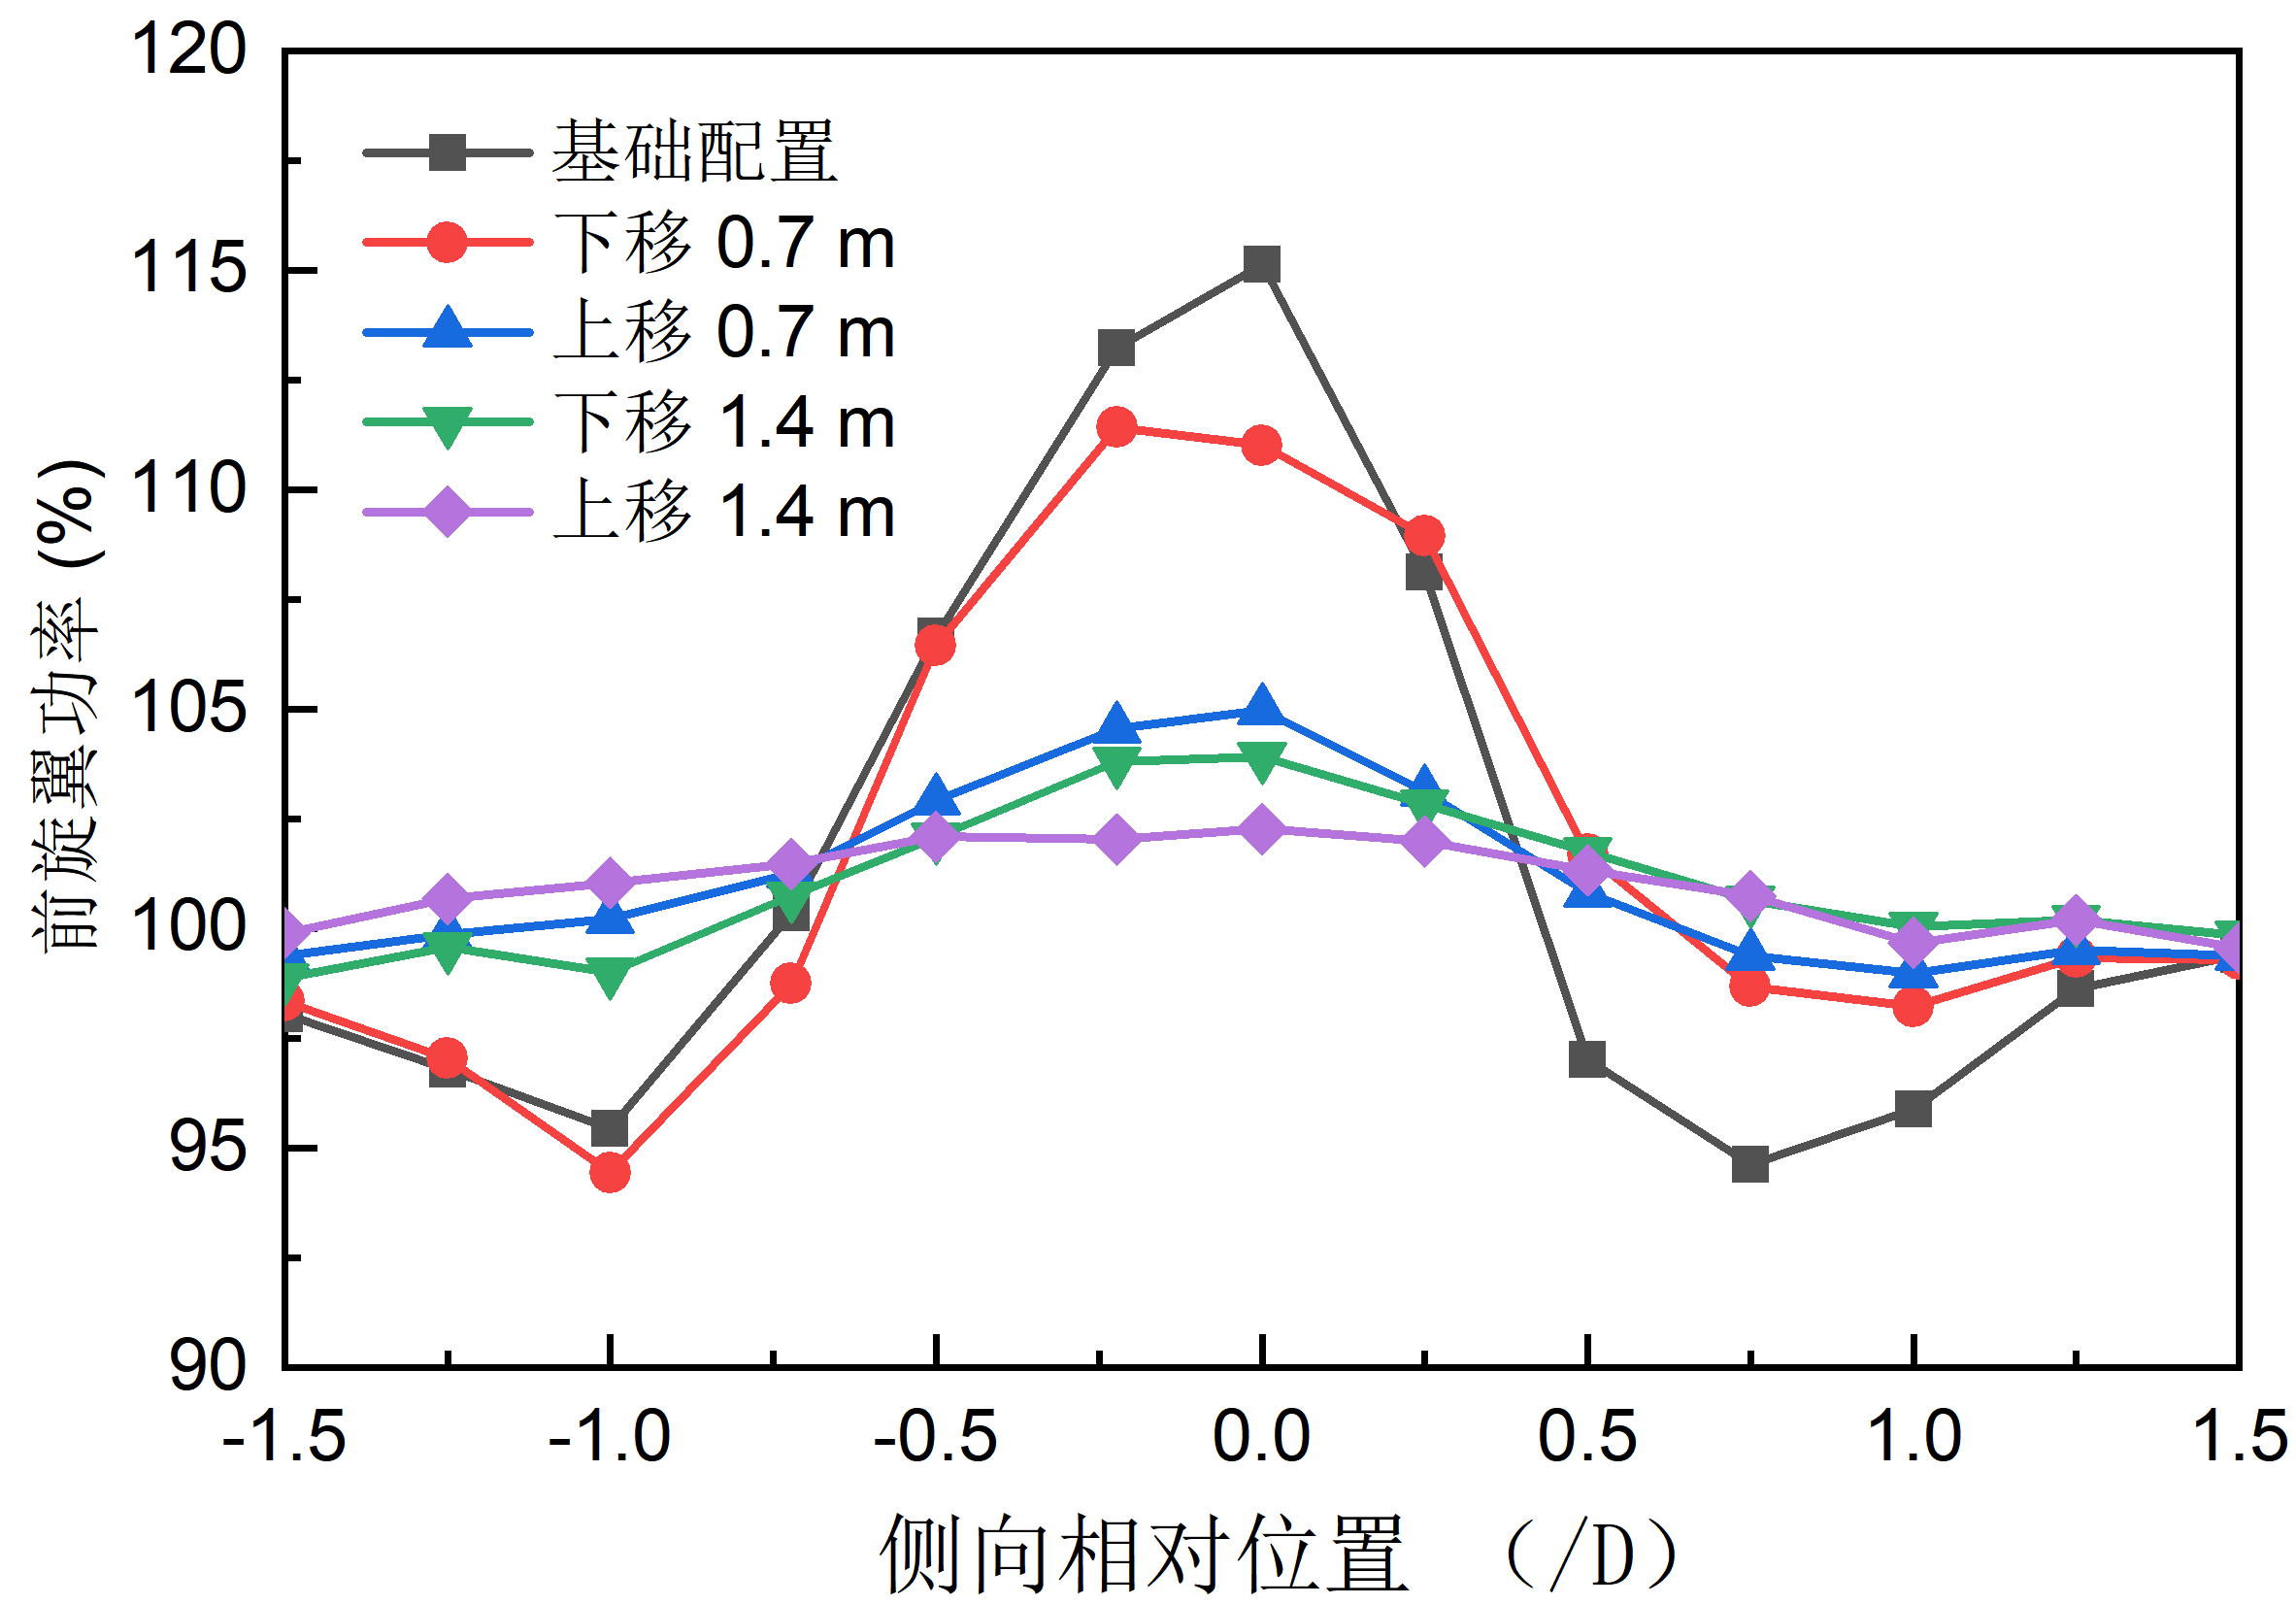
\includegraphics[width=7cm]{fig/figure_chap3/chap_3_5_4_8.png}}\quad
  \subfloat[后旋翼]{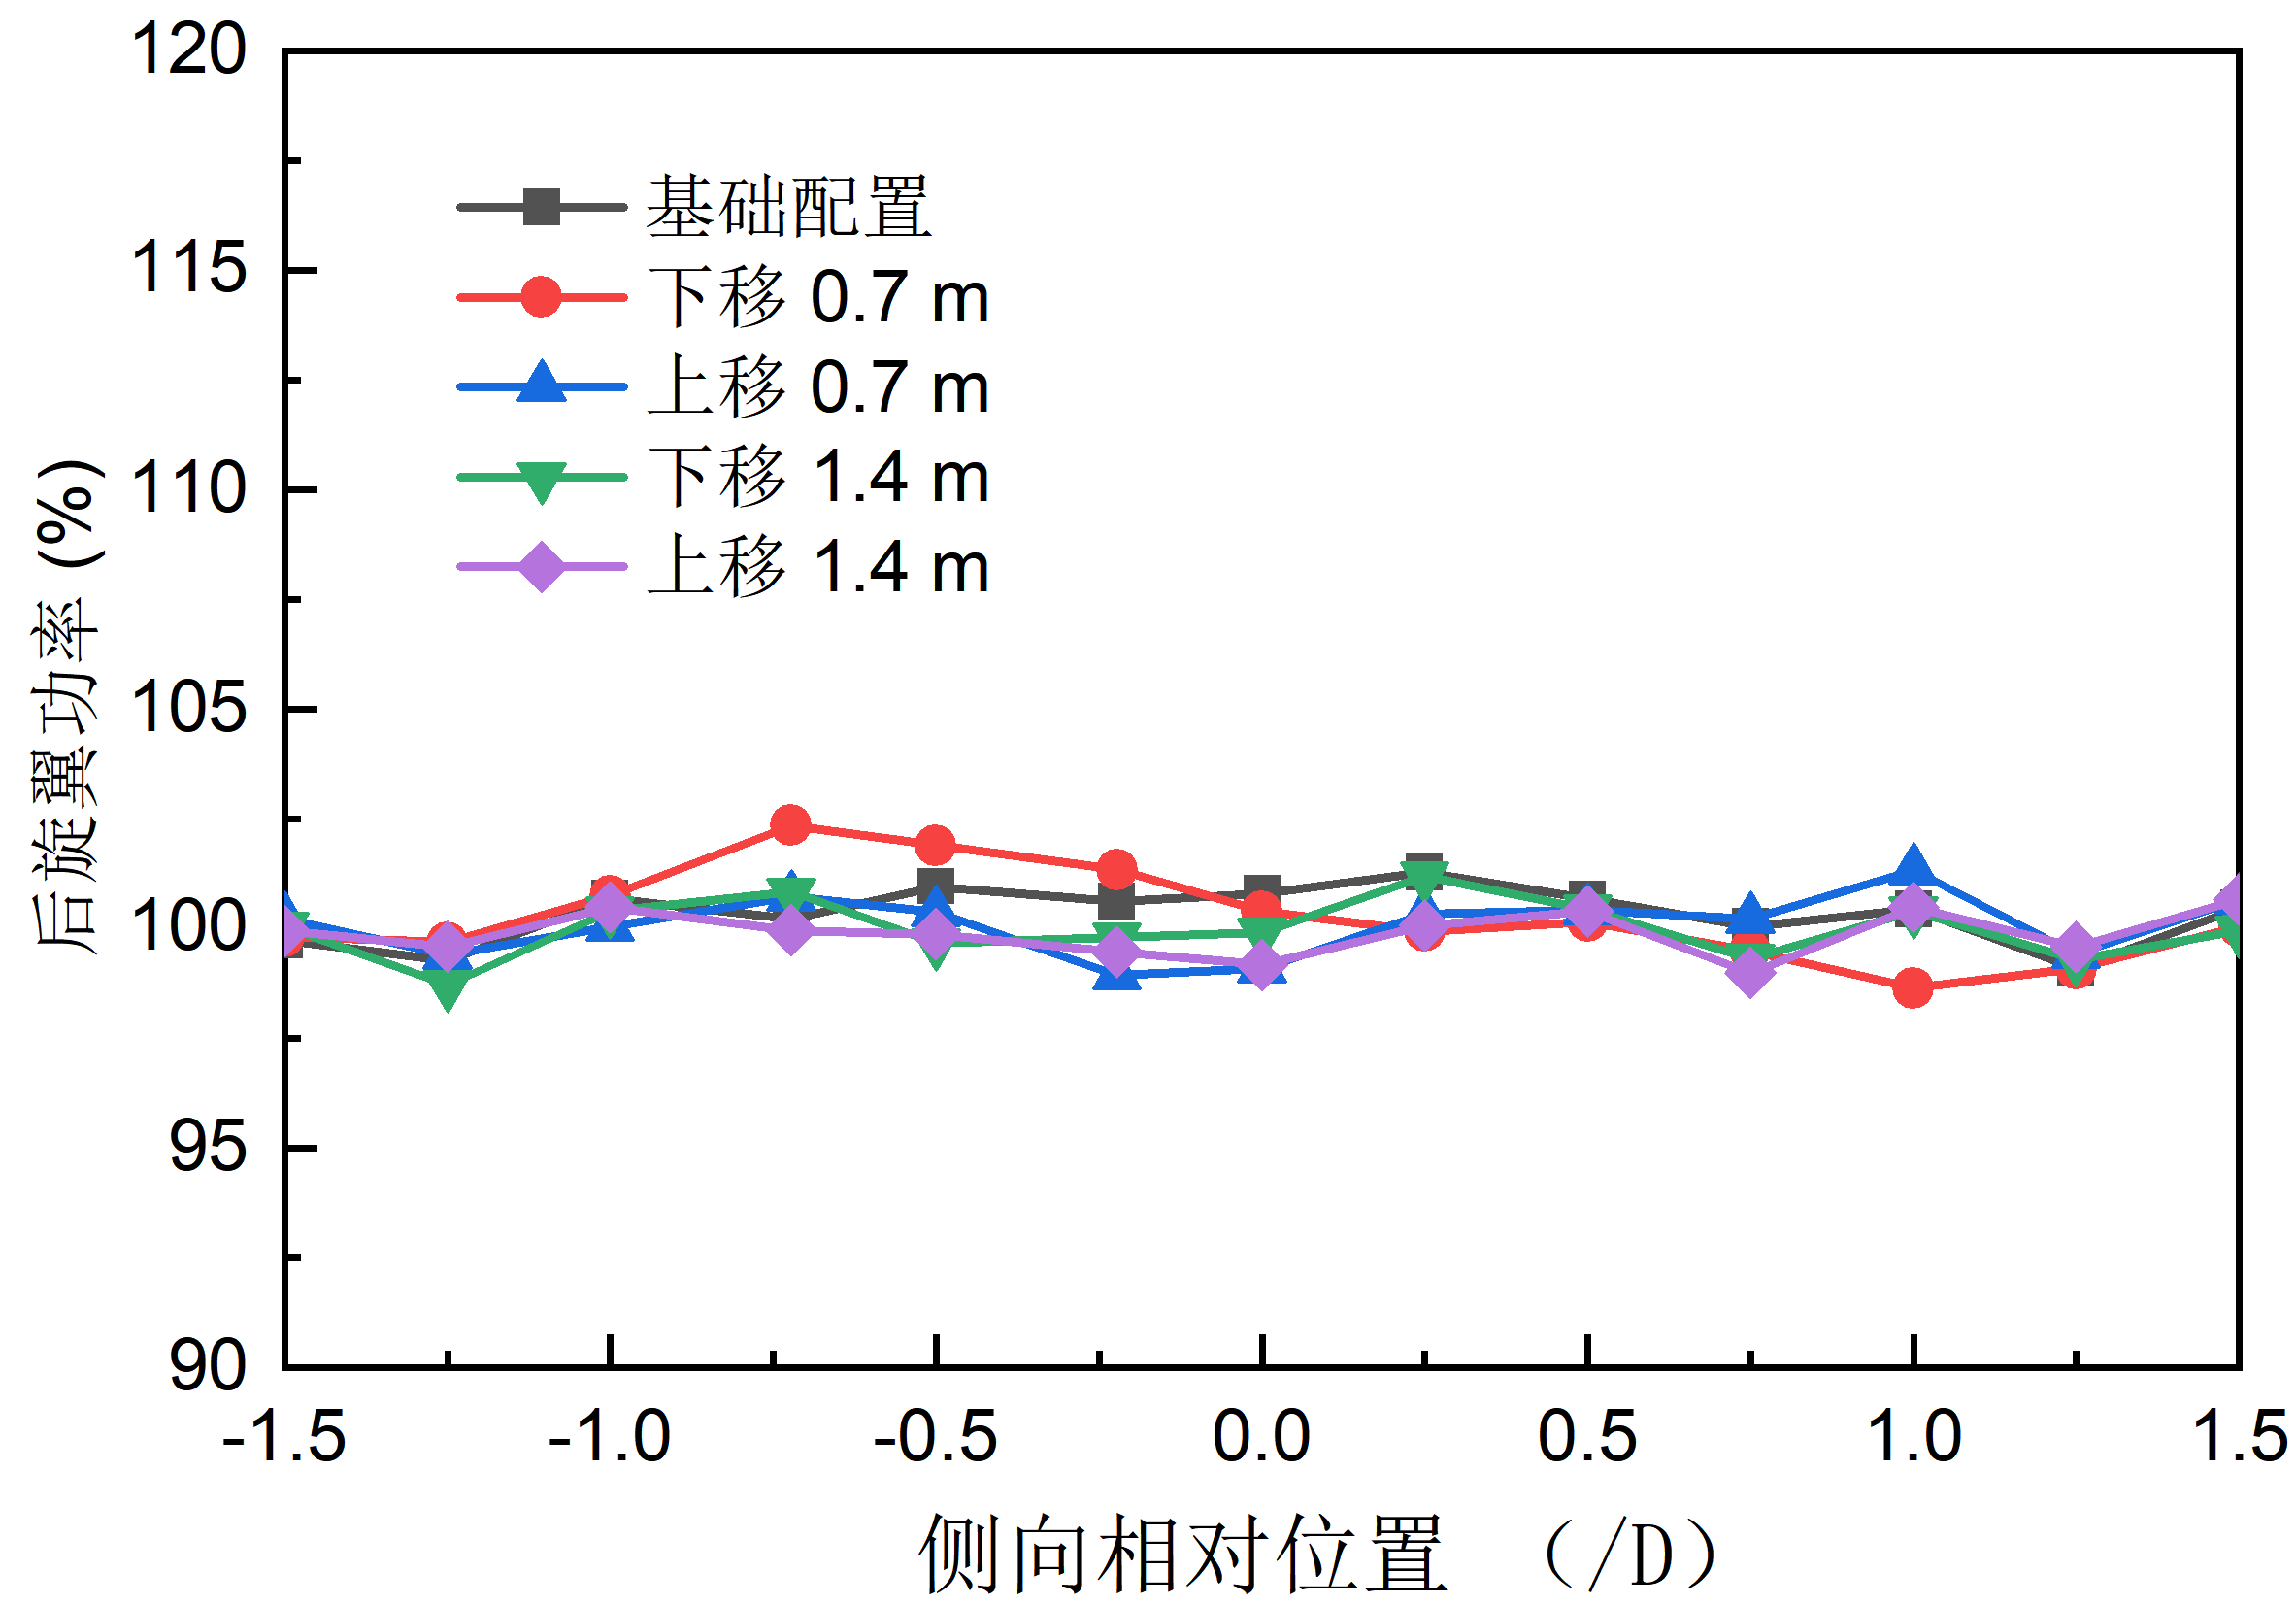
\includegraphics[width=7cm]{fig/figure_chap3/chap_3_5_4_9.png}}
  \caption{不同垂向相对位置下的旋翼功率}
  \label{fig:chap3_5_4_4}
\end{figure}
\subsection{基于气动干扰分析的协同吊挂系统队形推荐}
基于上面的气动干扰分析,前进比为0.1时,直升机1和直升机4间的侧向相对位置处于-1.5到-0.75倍的旋翼直径、0.75到1.5倍的旋翼直径时,有利于减少气动干扰、降低拉力损失、减少功率消耗。当直升机1和直升机4间的纵向相对距离大于2.5倍的旋翼直径、后方直升机比前侧直升机高0.5倍的旋翼直径时,气动干扰大幅减少,有利于提高性能。此外,考虑到前进比0.1时对应气动干扰相对严重的情况,因此以上结论对悬停、前进比小于0.1时均适用。

因此,横纵向相对位置越大或后侧直升机比前侧直升机垂向位置高时,有利于减小直升机协同吊挂系统间的气动干扰。这意味着图\ref{fig:chap3_5_5_1}所示的梯形队形或后侧直升机相对较高的矩形队形更佳。
\begin{figure}[!htb]
  \centering
  \subfloat[梯形队形]{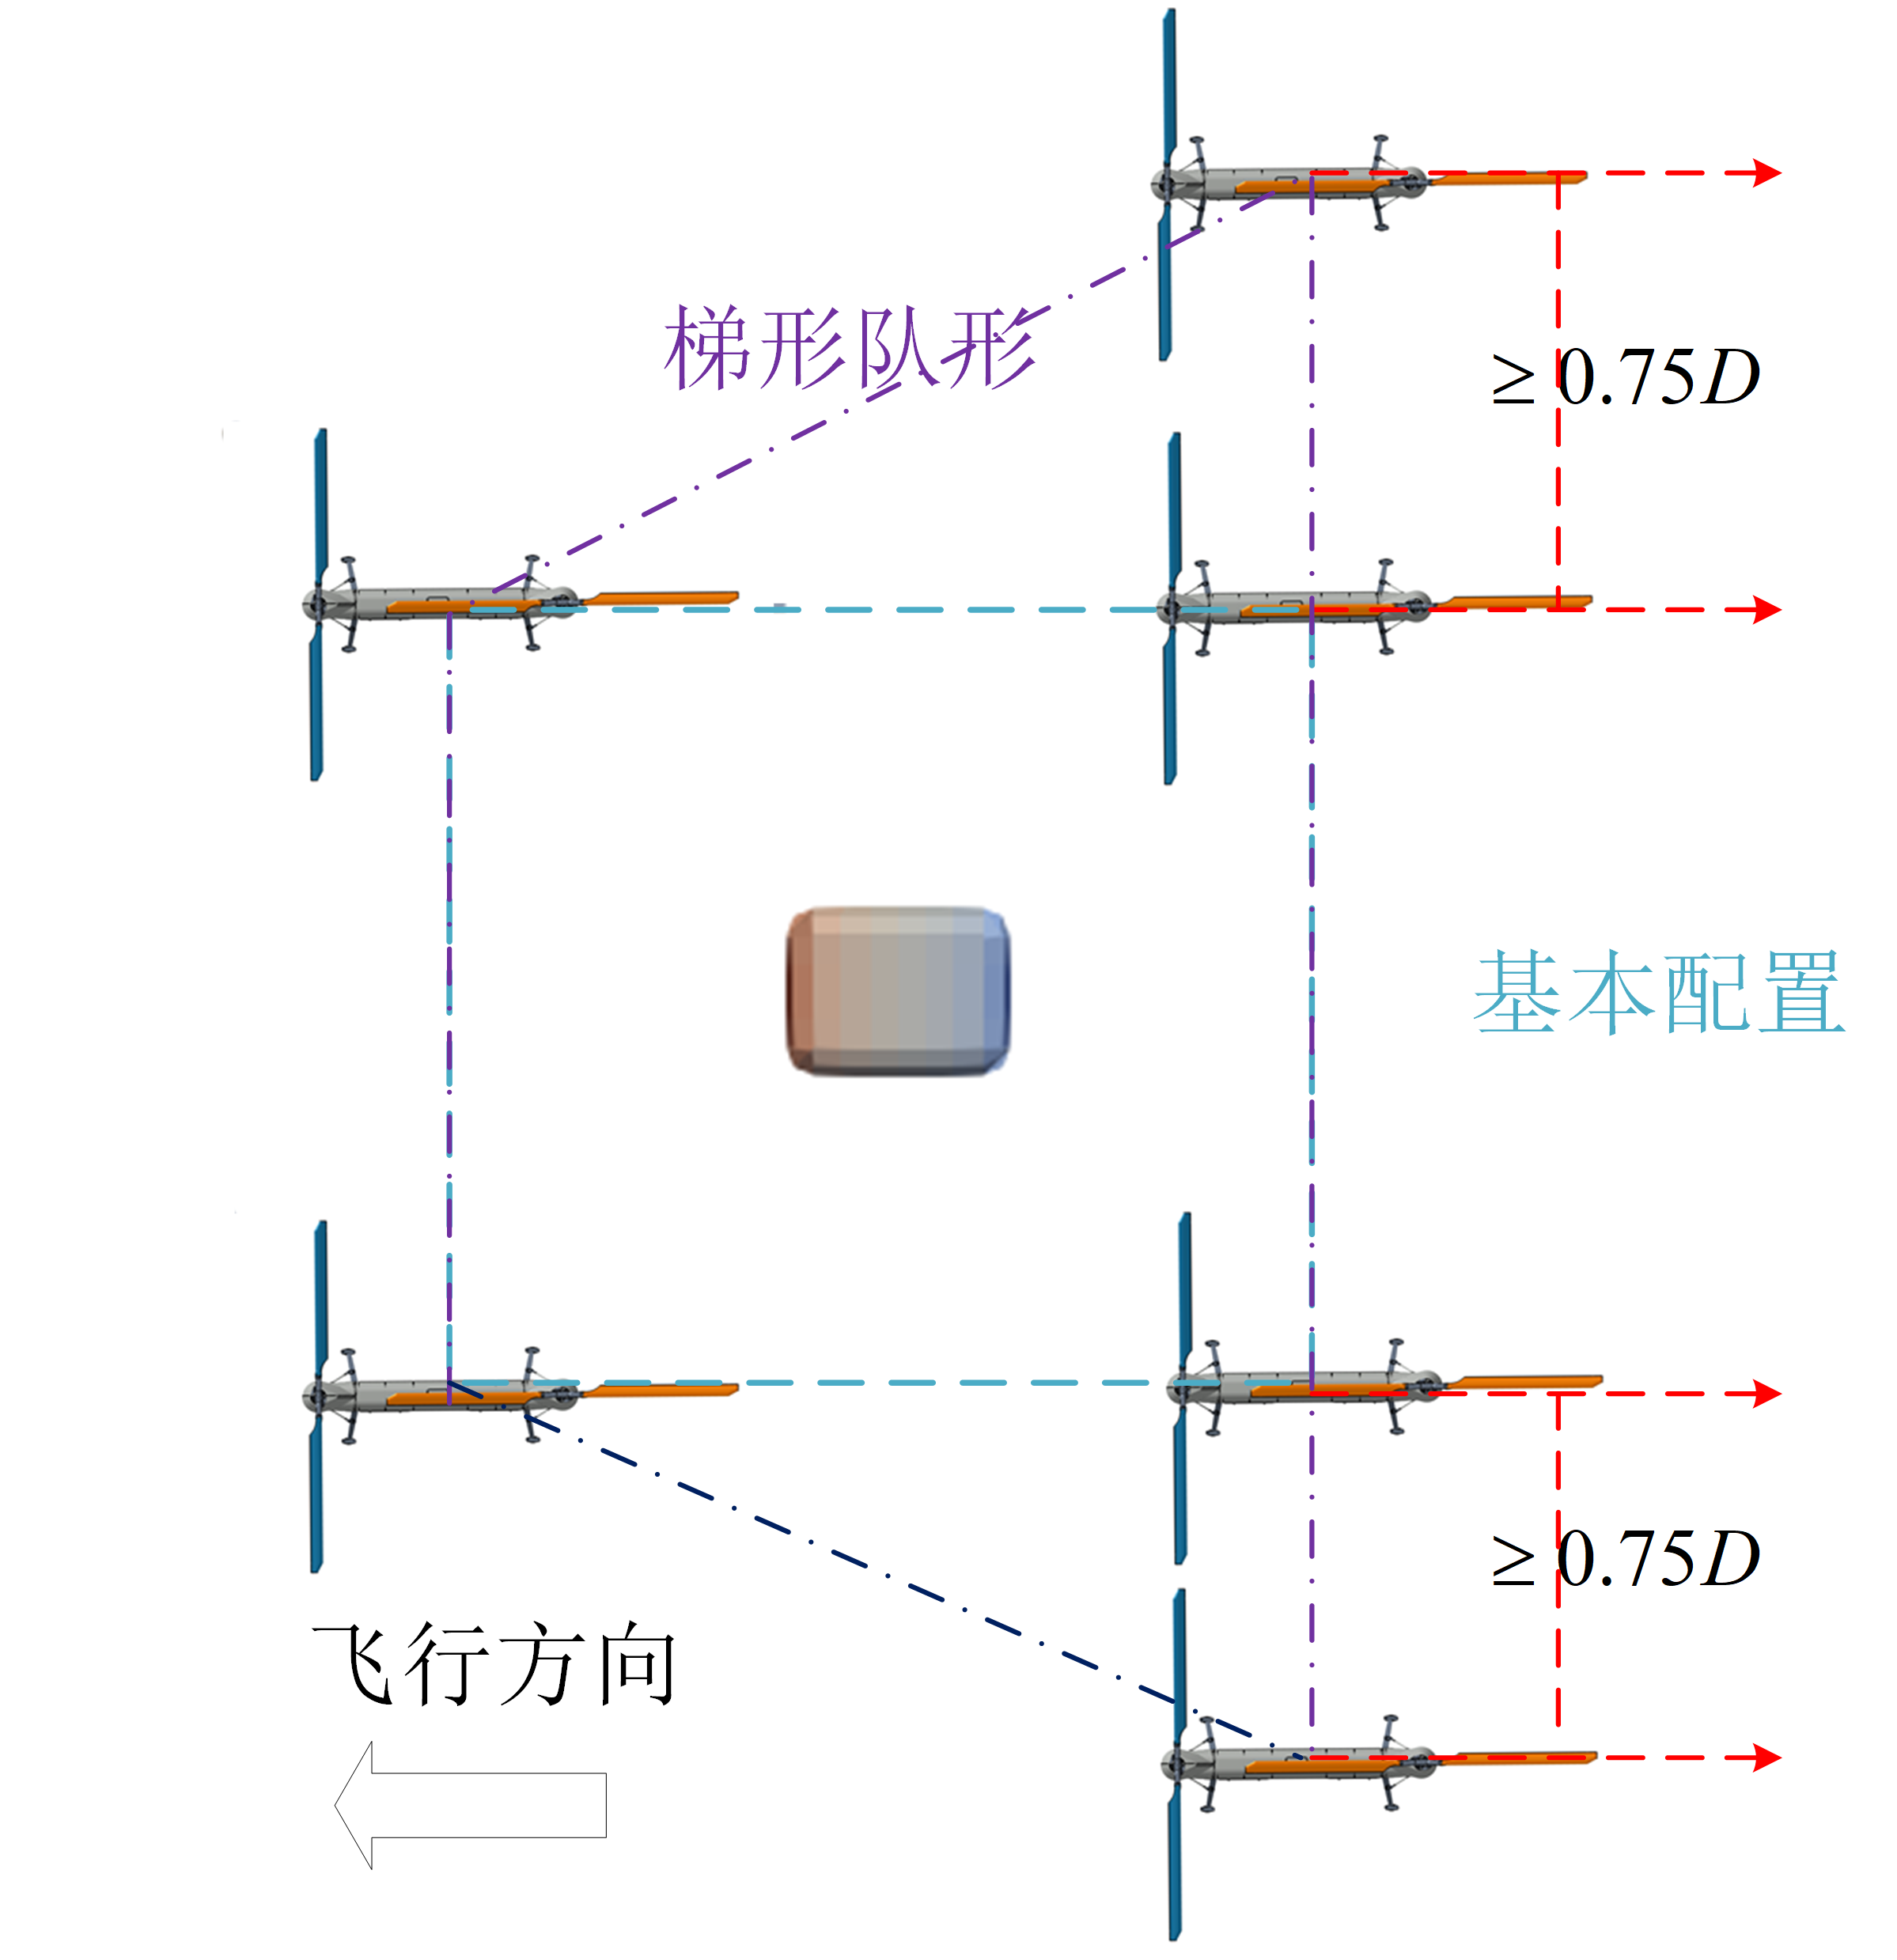
\includegraphics[width=6cm]{fig/figure_chap3/chap_3_5_5_1.png}}\quad
  \subfloat[矩形队形]{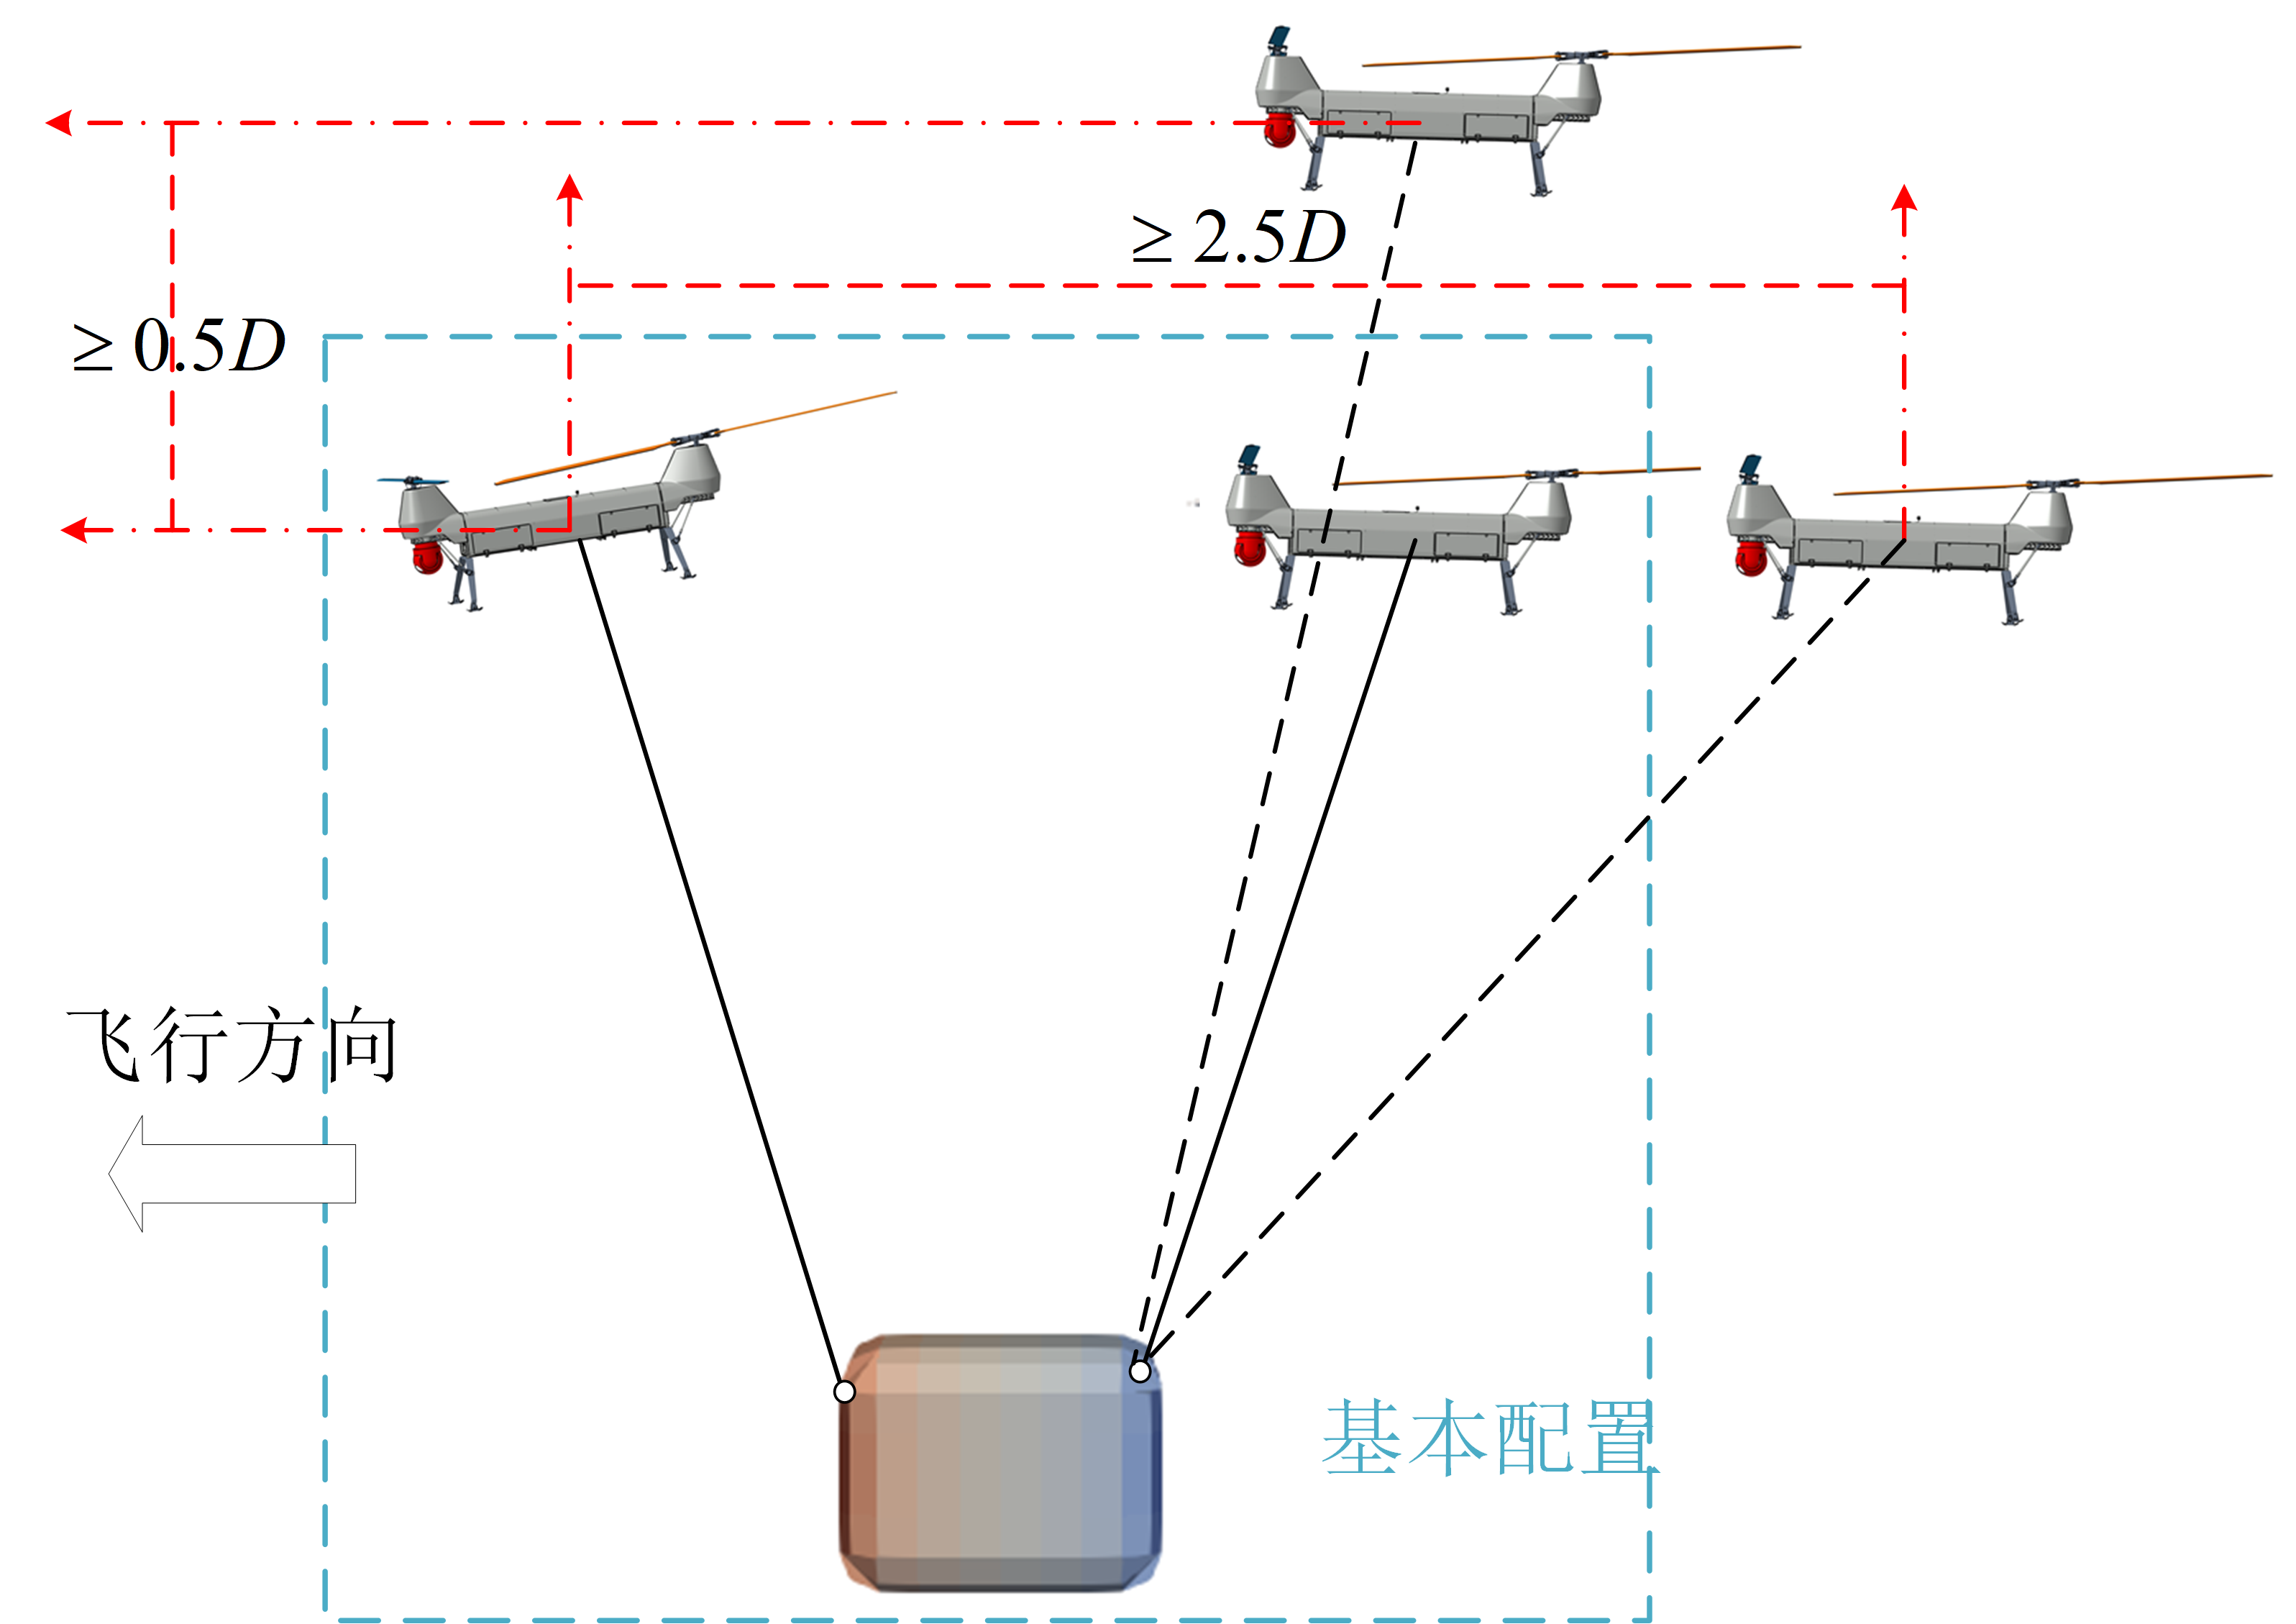
\includegraphics[width=8cm]{fig/figure_chap3/chap_3_5_5_2.png}}
  \caption{基于气动干扰分析的协同吊挂系统队形推荐}
  \label{fig:chap3_5_5_1}
\end{figure}

\section{本章小结}
本小节给出了直升机协同吊挂系统的配平方法,分析了整个系统的稳定性和操作性,并在配平基础了开展了系统的气动干扰分析,从气动干扰角度给出了直升机协同吊挂系统的推荐队形,对下文控制策略的设计、吊挂负载的合理分配等均奠定了基础。主要包括
\begin{enumerate}
  \item 在配平的基础了,基于涡方法分析了直升机协同吊挂系统的气动干扰情况,并指出本文研究的四直升机协同吊挂系统,前飞时的前后排列的直升机间气动干扰更为严重。为此,以前进比0.1(前飞速度10 m/s)为例,分析了不同侧向、纵向、垂向相对位置对气动干扰的影响。基于以上分析,指出从减小气动干扰的角度,梯形队形或后侧直升机相对较高的矩形队形更佳。
\end{enumerate}